% Options for packages loaded elsewhere
\PassOptionsToPackage{unicode}{hyperref}
\PassOptionsToPackage{hyphens}{url}
\PassOptionsToPackage{dvipsnames,svgnames,x11names}{xcolor}
%
\documentclass[
]{report}
\usepackage{amsmath,amssymb}
\usepackage{iftex}
\ifPDFTeX
  \usepackage[T1]{fontenc}
  \usepackage[utf8]{inputenc}
  \usepackage{textcomp} % provide euro and other symbols
\else % if luatex or xetex
  \usepackage{unicode-math} % this also loads fontspec
  \defaultfontfeatures{Scale=MatchLowercase}
  \defaultfontfeatures[\rmfamily]{Ligatures=TeX,Scale=1}
\fi
\usepackage{lmodern}
\ifPDFTeX\else
  % xetex/luatex font selection
\fi
% Use upquote if available, for straight quotes in verbatim environments
\IfFileExists{upquote.sty}{\usepackage{upquote}}{}
\IfFileExists{microtype.sty}{% use microtype if available
  \usepackage[]{microtype}
  \UseMicrotypeSet[protrusion]{basicmath} % disable protrusion for tt fonts
}{}
\makeatletter
\@ifundefined{KOMAClassName}{% if non-KOMA class
  \IfFileExists{parskip.sty}{%
    \usepackage{parskip}
  }{% else
    \setlength{\parindent}{0pt}
    \setlength{\parskip}{6pt plus 2pt minus 1pt}}
}{% if KOMA class
  \KOMAoptions{parskip=half}}
\makeatother
\usepackage{xcolor}
\usepackage[margin=1in]{geometry}
\usepackage{longtable,booktabs,array}
\usepackage{calc} % for calculating minipage widths
% Correct order of tables after \paragraph or \subparagraph
\usepackage{etoolbox}
\makeatletter
\patchcmd\longtable{\par}{\if@noskipsec\mbox{}\fi\par}{}{}
\makeatother
% Allow footnotes in longtable head/foot
\IfFileExists{footnotehyper.sty}{\usepackage{footnotehyper}}{\usepackage{footnote}}
\makesavenoteenv{longtable}
\usepackage{graphicx}
\makeatletter
\def\maxwidth{\ifdim\Gin@nat@width>\linewidth\linewidth\else\Gin@nat@width\fi}
\def\maxheight{\ifdim\Gin@nat@height>\textheight\textheight\else\Gin@nat@height\fi}
\makeatother
% Scale images if necessary, so that they will not overflow the page
% margins by default, and it is still possible to overwrite the defaults
% using explicit options in \includegraphics[width, height, ...]{}
\setkeys{Gin}{width=\maxwidth,height=\maxheight,keepaspectratio}
% Set default figure placement to htbp
\makeatletter
\def\fps@figure{htbp}
\makeatother
\setlength{\emergencystretch}{3em} % prevent overfull lines
\providecommand{\tightlist}{%
  \setlength{\itemsep}{0pt}\setlength{\parskip}{0pt}}
\setcounter{secnumdepth}{5}
\usepackage{titlesec, blindtext, color, float}

\titleformat{\chapter}[display]
  {\Huge\bfseries}
  {}
  {0pt}
  {\thechapter.\ }

\titleformat{name=\chapter,numberless}[display]
  {\Huge\bfseries}
  {}
  {0pt}
  {}

\titlespacing*{\chapter}{0pt}{0pt}{40pt}

\renewcommand{\bibname}{References}
\usepackage{booktabs}
\usepackage{longtable}
\usepackage{array}
\usepackage{multirow}
\usepackage{wrapfig}
\usepackage{float}
\usepackage{colortbl}
\usepackage{pdflscape}
\usepackage{tabu}
\usepackage{threeparttable}
\usepackage{threeparttablex}
\usepackage[normalem]{ulem}
\usepackage{makecell}
\usepackage{xcolor}
\ifLuaTeX
  \usepackage{selnolig}  % disable illegal ligatures
\fi
\usepackage[]{natbib}
\bibliographystyle{apalike}
\usepackage{bookmark}
\IfFileExists{xurl.sty}{\usepackage{xurl}}{} % add URL line breaks if available
\urlstyle{same}
\hypersetup{
  pdftitle={Ovarian Cancer Histotypes: Report of Statistical Findings},
  pdfauthor={Derek Chiu},
  colorlinks=true,
  linkcolor={Maroon},
  filecolor={Maroon},
  citecolor={Blue},
  urlcolor={Blue},
  pdfcreator={LaTeX via pandoc}}

\title{Ovarian Cancer Histotypes: Report of Statistical Findings}
\author{Derek Chiu}
\date{2024-05-17}

\begin{document}
\maketitle

{
\hypersetup{linkcolor=}
\setcounter{tocdepth}{1}
\tableofcontents
}
\listoffigures
\listoftables
\chapter*{Preface}\label{preface}
\addcontentsline{toc}{chapter}{Preface}

This report of statistical findings describes the classification of ovarian cancer histotypes using data from NanoString CodeSets.

Marina Pavanello conducted the initial exploratory data analysis, Cathy Tang implemented class imbalance techniques, Derek Chiu conducted the normalization and statistical analysis, and Lauren Tindale and Aline Talhouk are the project leads.

\chapter{Introduction}\label{introduction}

Ovarian cancer has five major histotypes: high-grade serous carcinoma (HGSC), low-grade serous carcinoma (LGSC), endometrioid carcinoma (ENOC), mucinous carcinoma (MUC), and clear cell carcinoma (CCOC). A common problem with classifying these histotypes is that there is a class imbalance issue. HGSC dominates the distribution, commonly accounting for 70\% of cases in many patient cohorts, while the other four histotypes are spread over the rest of the cases. Subsampling methods like up-sampling, down-sampling, and SMOTE can be used to mitigate this problem.

The supervised learning is performed under a consensus framework: we consider various classification algorithms and use evaluation metrics like accuracy, F1-score, Kappa, and G-mean to inform the decision of which methods to carry forward for prediction in confirmation and validation sets.

\chapter{Methods}\label{methods}

\section{Pre-Processing}\label{pre-processing}

\subsection{Case Selection}\label{case-selection}

Raw data comes from three NanoString CodeSets (CS): CS1, CS2, and CS3. We divide the data into training, confirmation, and validation sets by using samples from these sets of cohorts:

\begin{itemize}
\tightlist
\item
  Training

  \begin{itemize}
  \tightlist
  \item
    CS1: MAYO, OOU, OOUE, VOA, MTL
  \item
    CS2: MAYO, OOU, OOUE, OVAR3, VOA, ICON7, JAPAN, MTL, POOL-CTRL
  \item
    CS3: OOU, OOUE, VOA, POOL-1, POOL-2, POOL-3
  \end{itemize}
\item
  Confirmation:

  \begin{itemize}
  \tightlist
  \item
    CS3: TNCO
  \end{itemize}
\item
  Validation:

  \begin{itemize}
  \tightlist
  \item
    CS3: DOVE4
  \end{itemize}
\end{itemize}

\subsection{Quality Control}\label{quality-control}

Samples that failed any of the following NanoString quality control conditions were removed:

\begin{itemize}
\tightlist
\item
  \texttt{linFlag}: linearity of positive controls with positive control concentrations is less than 0.95, or linearity measures are unknown
\item
  \texttt{imagingFlag}: percent of field of view is less than 75\%
\item
  \texttt{spcFlag}: smallest positive control is less than the lower limit of detection (negative control average expression less two times the negative control standard deviation), or negative control average expression equals zero
\item
  \texttt{normFlag}: signal to noise ratio less than 100, or percent of genes detected is less than 50. Note: these thresholds were determined by examining the \hyperref[gd-vs.-snr]{\%GD vs.~SNR} relationship below.
\end{itemize}

\subsection{Normalization}\label{normalization}

The full training set (n=1246) is comprised of data from CodeSets (CS) 1, 2, and 3. All CodeSets were first normalized to housekeeping genes, then different approaches were taken for subsequent normalizations of each CodeSet.

CS1 was normalized to CS3 using five ``Random1'' reference samples. These reference samples are randomly selected from CS1 among all samples in the three CodeSets that share common otta IDs, such that we obtain one sample from each of the five histotypes. Then, we use the reference-based method to normalize CS1 to CS3 across their common genes, for the remaining expression samples \citet{talhouk2016}.

Similarly, CS2 was normalized to CS3 using the same ``Random1'' reference samples, now taken from CS2. Normalization was performed across common genes between CS2 and CS3.

For CS3, we first split the dataset into three sites: Vancouver, USC, and AOC. We use the CS3-Vancouver subset as a ``reference standard'', and normalized CS3-USC and CS3-AOC to CS3-Vancouver using a ``Random1'' reference set randomly selected among samples common between Vancouver, USC, and AOC. Finally, the CS3-Vancouver expression samples are included in the training set without further normalization.

\subsection{Final Processing}\label{final-processing}

We map ovarian histotypes to all remaining samples and keep the major histotypes for building the predictive model: high-grade serous carcinoma (HGSC), clear cell ovarian caricoma (CCOC), endometrioid ovarian carcinoma (ENOC), low-grade serous carcinoma (LGSC), mucinous carcinoma (MUC).

Duplicate cases (two samples with the same ottaID) were removed before generating the final training set to use for fitting the classification models. All CS3 cases were preferred over CS1 and CS2, and CS3-Vancouver cases were preferred over CS3-AOC and CS3-USC when selecting duplicates.

The final training set used only genes that were common across all three CodeSets.

\section{Classifiers}\label{classifiers}

We use 4 classification algorithms in the supervised learning framework for the Training Set. The pipeline was run using SLURM batch jobs submitted to a partition on a CentOS 7 server. All resampling techniques, pre-processing, model specification, hyperparameter tuning, and evaluation metrics were implemented using the \texttt{tidymodels} suite of packages. The classifiers we used are:

\begin{itemize}
\tightlist
\item
  Random Forest (\texttt{rf})
\item
  Support Vector Machine (\texttt{svm})
\item
  XGBoost (\texttt{xgb})
\item
  Regularized Multinomial Regression (\texttt{mr})
\end{itemize}

\subsection{Resampling of Training Set}\label{resampling-of-training-set}

We used a nested cross-validation design to assess each classifier while also performing hyperparameter tuning. An outer 5-fold CV stratified by histotype was used together with an inner 5-fold CV with 2 repeats stratified by histotype. This design was chosen such that the test sets of the inner resamples would still have a reasonable number of samples belonging to the smallest minority class.

The outer resampling method cannot be the bootstrap, because the inner training and inner test sets will likely contain the same samples as a result of sampling with replacement in the outer training set. This phenomenon might result in inflated performance as some observations are used both to train and evaluate the hyperparameter tuning in the inner loop.

\subsection{Hyperparameter Tuning}\label{hyperparameter-tuning}

The following specifications for each classifier were used for tuning hyperparameters:

\begin{itemize}
\tightlist
\item
  \texttt{rf} and \texttt{xgb}: The number of trees were fixed at 500. Other hyperparameters were tuned across 10 randomly selected points in a latin hypercube design.
\item
  \texttt{svm}: Both the cost and sigma hyperparameters were tuned across 10 randomly selected points in a latin hypercube design. We tuned the cost parameter in the range {[}1, 8{]}. The range for tuning the sigma parameter was obtained from the 10\% and 90\% quantiles of the estimation using the \texttt{kernlab::sigest()} function.
\item
  \texttt{mr}: We generated 10 randomly selected points in a latin hypercube design for the penalty (lambda) parameter. Then, we generated 10 evenly spaced points in {[}0, 1{]} for the mixture (alpha) parameter in the regularized multinomial regression model. These two sets of 10 points were crossed to generate a tuning grid of 100 points.
\end{itemize}

The hyperparameter combination that resulted in the highest average F1-score across the inner training sets was selected for each classifier to use as the model for assessing prediction performance in the outer training loop.

\subsection{Subsampling}\label{subsampling}

Here are the specifications of the subsampling methods used to handle class imbalance:

\begin{itemize}
\tightlist
\item
  None: No subsampling is performed
\item
  Down-sampling: All levels except the minority class are sampled down to the same frequency as the minority class
\item
  Up-sampling: All levels except the majority class are sampled up to the same frequency as the majority class
\item
  SMOTE: All levels except the majority class have synthetic data generated until they have the same frequency as the majority class
\item
  Hybrid: All levels except the majority class have synthetic data generated up to 50\% of the frequency of the majority class, then the majority class is sampled down to the same frequency as the rest.
\end{itemize}

The figure below helps visualize how the distribution of classes changes when we apply subsampling techniques to handle class imbalance:

\begin{figure}[H]

{\centering 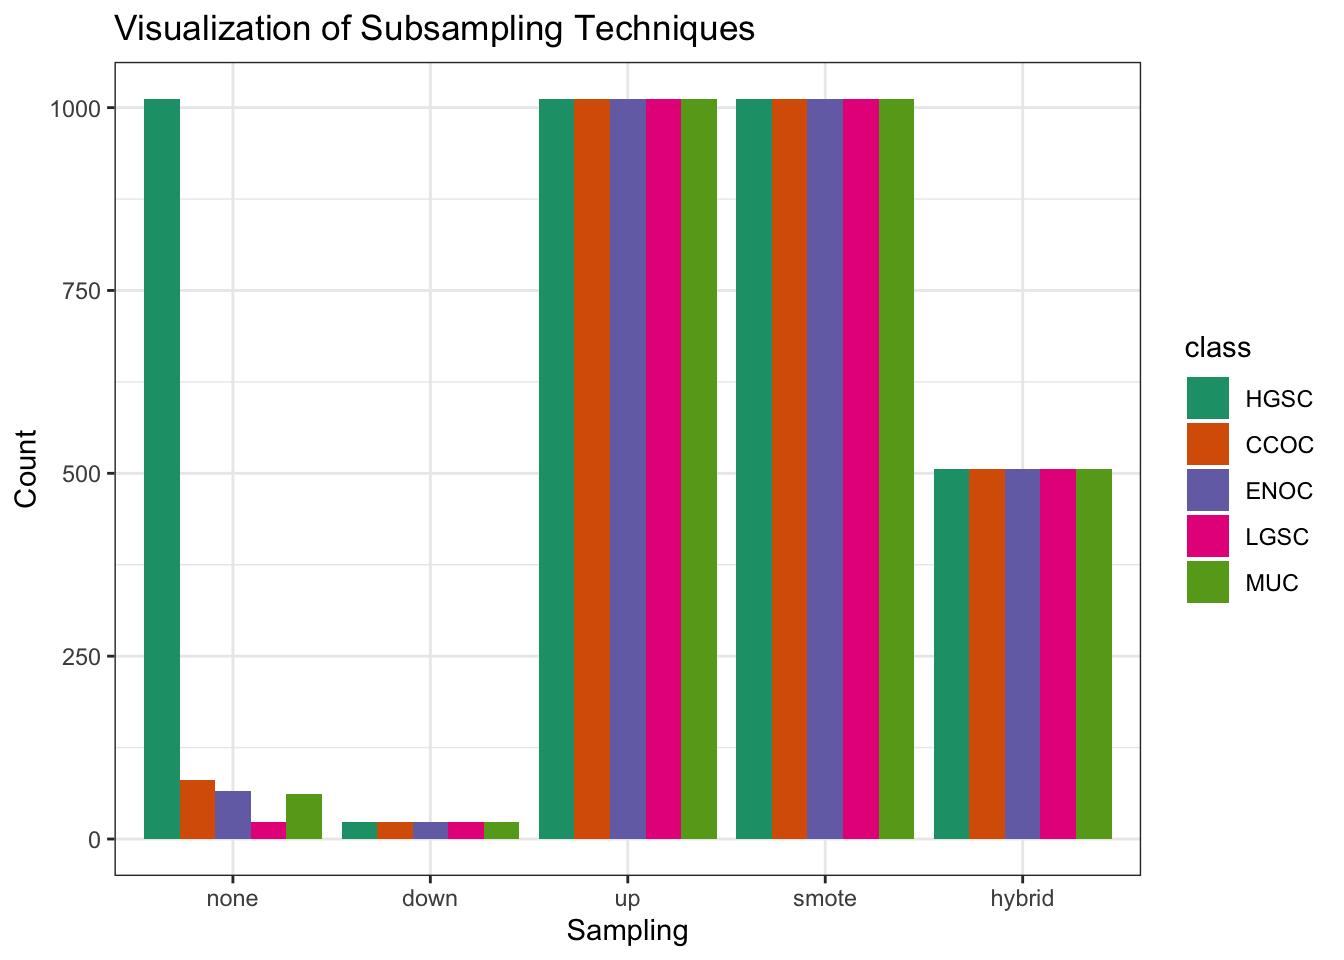
\includegraphics{OV_Histotypes_RSF_files/figure-latex/sampling-1} 

}

\caption{Visualization of Subsampling Techniques}\label{fig:sampling}
\end{figure}

\subsection{Workflows}\label{workflows}

The 4 \textbf{algorithms} and 5 \textbf{subsampling} methods are crossed to create 20 different classification \textbf{workflows}. For example, the \texttt{hybrid\_xgb} workflow is a classifier that first pre-processes a training set by applying a hybrid subsampling method, and then proceeds to use the XGBoost algorithm to classify ovarian histotypes.

\section{Two-Step Algorithm}\label{two-step-algorithm}

The HGSC histotype comprises of approximately 80\% of cases among ovarian carcinoma patients, while the remaining 20\% of cases are relatively, evenly distributed among ENOC, CCOC, LGSC, and MUC histotypes. We can implement a two-step algorithm as such:

\begin{itemize}
\tightlist
\item
  Step 1: use binary classification for HGSC vs.~non-HGSC
\item
  Step 2: use multinomial classification for the remaining non-HGSC classes
\end{itemize}

Let

\[
\begin{aligned}
& X_k = \text{Training data with k classes}  \\
& C_k = \text{Class with highest}\;F_1\;\text{score from training}\;X_k \\
& W_k = \text{Workflow associated with}\;C_k
\end{aligned}
\label{eq:sequential}
\]

Figure \ref{fig:two-step-flowchart} shows how the two-step algorithm works:

\begin{figure}[H]

{\centering \includegraphics{OV_Histotypes_RSF_files/figure-latex/two-step-flowchart-1} 

}

\caption{Two-Step Algorithm}\label{fig:two-step-flowchart}
\end{figure}

Although the class imbalance problem is mostly eliminated in Step 2 after removing the HGSC cases, we still use the same subsampling method in Step 2 as was used in Step 1 to keep the algorithm consistent.

\subsection{Aggregating Predictions}\label{aggregating-predictions}

The aggregation for two-step predictions is quite straightforward:

\begin{enumerate}
\def\labelenumi{\arabic{enumi}.}
\tightlist
\item
  Predict HGSC vs.~non-HGSC
\item
  Among all non-HGSC cases, predict CCOC vs.~LGSC vs.~MUC vs.~ENOC
\end{enumerate}

\begin{figure}[H]

{\centering \includegraphics{OV_Histotypes_RSF_files/figure-latex/two-step-predictions-1} 

}

\caption{Aggregating Predictions for Two-Step Algorithm}\label{fig:two-step-predictions}
\end{figure}

\section{Sequential Algorithm}\label{sequential-algorithm}

Instead of training on k classes simultaneously using multinomial classifiers, we can use a sequential algorithm that performs k-1 one-vs-all binary classifications iteratively to obtain a final prediction of all cases. At each step in the sequence, we classify one class vs.~all other classes, where the classes that make up the ``other'' class are those not equal to the current ``one'' class and excluding all ``one'' classes from previous steps. For example, if the ``one'' class in step 1 was HGSC, the ``other'' classes would include CCOC, ENOC, LGSC, and MUC. If the ``one'' class in step 2 was CCOC, the ``other'' classes include ENOC, LGSC, and MUC.

The order of classes and workflows to use at each step in the sequential algorithm must be determined using a retraining procedure. After removing the data associated with a particular class, we retrain using the remaining data using multinomial classifiers as described before. The class and workflow to use for the next step in the sequence is selected based on the best per-class evaluation metric value (e.g.~F1-score).

Figure \ref{fig:sequential-flowchart} illustrates how the sequential algorithm works for K=5, using ovarian histotypes as an example for the classes.

\begin{figure}[H]

{\centering \includegraphics{OV_Histotypes_RSF_files/figure-latex/sequential-flowchart-1} 

}

\caption{Sequential Algorithm}\label{fig:sequential-flowchart}
\end{figure}

The subsampling method used in the first step of the sequential algorithm is used in all subsequent steps in order to maintain data pre-processing consistency. As a result, we are only comparing classification algorithms within one subsampling method across the entire sequential algorithm.

\subsection{Aggregating Predictions}\label{aggregating-predictions-1}

We have to aggregate the one-vs-all predictions from each of the sequential algorithm workflows in order to obtain a final class prediction on a holdout test set. Each sequential workflow has to be assessed on every sample to ensure that cases classified into the ``all'' class from a previous step of the sequence are eventually assigned a predicted class. For example, say that based on certain class-specific metrics we determined that the order of classes in the sequential algorithm was to predict HGSC vs.~non-HGSC, CCOC vs.~non-CCOC, LGSC vs.~non-LGSC, and then MUC vs.~ENOC. Figure \ref{fig:sequential-predictions} illustrates how the final predictions are assigned:

\begin{figure}[H]

{\centering \includegraphics{OV_Histotypes_RSF_files/figure-latex/sequential-predictions-1} 

}

\caption{Aggregating Predictions for Sequential Algorithm}\label{fig:sequential-predictions}
\end{figure}

\section{Gene Optimization}\label{gene-optimization}

We want to discover an optimal set of genes for the classifiers while including specific genes from other studies such as PrOTYPE and SPOT. A total of 72 genes are used in the classifier training set.

There are 16 genes in the classifier set that overlap with the PrOTYPE classifier: COL11A1, CD74, CD2, TIMP3, LUM, CYTIP, COL3A1, THBS2, TCF7L1, HMGA2, FN1, POSTN, COL1A2, COL5A2, PDZK1IP1, FBN1.

There are also 13 genes in the classifier set that overlap with the SPOT signature: HIF1A, CXCL10, DUSP4, SOX17, MITF, CDKN3, BRCA2, CEACAM5, ANXA4, SERPINE1, TCF7L1, CRABP2, DNAJC9.

We obtain a total of 28 genes from the union of PrOTYPE and SPOT genes that we want to include in the final classifier, regardless of model performance. We then incrementally add genes one at a time from the remaining 44 candidate genes based on an overall variable importance rank to the set of 28 base genes and recalculate performance metrics. The number of genes at which the performance peaks or starts to plateau may indicate an optimal gene set model for us to compare with the full set model.

\subsection{Variable Importance}\label{variable-importance}

Variable importance is calculated using either a model-based approach if it is available, or a permutation-based VI score otherwise. The variable importance scores are averaged across the outer training folds, and then ranked from highest to lowest.

For the sequential and two-step classifiers, we calculate an overall VI rank by taking the cumulative union of genes at each variable importance rank across all sequences, until all genes have been included.

The variable importance measures are:

\begin{itemize}
\item
  Random Forest: impurity measure (Gini index)
\item
  XGBoost: gain (fractional contribution of each feature to the model based on the total gain of the corresponding features's splits)
\item
  SVM: permutation based p-values
\item
  Multinomial regression: absolute value of estimated coefficients at cross-validated lambda value
\end{itemize}

\section{Performance Evaluation}\label{performance-evaluation}

\subsection{Class Metrics}\label{class-metrics}

We use the accuracy, sensitivity, specificity, F1-score, kappa, balanced accuracy, and geometric mean, as class metrics to measure both training and test performance between different workflows. Multiclass extensions of these metrics can be calculated except for F1-score, where we use macro-averaging to obtain an overall metric. Class-specific metrics are calculated by recoding classes into one-vs-all categories for each class.

\subsubsection{Accuracy}\label{accuracy}

The accuracy is defined as the proportion of correct predictions out of all cases:

\[
\text{accuracy} = \frac{TP}{TP + FP + FN + TN}
\label{eq:accuracy}
\]

\subsubsection{Sensitivity}\label{sensitivity}

Sensitivity is the proportional of correctly predicted positive cases, out of all cases that were truly positive

\[
\text{sensitivity} = \frac{TP}{TP + FN}
\label{eq:sens}
\]

\subsubsection{Specificity}\label{specificity}

Specificity is the proportional of correctly predicted negative cases, out of all cases that were truly negative.

\[
\text{specificity} = \frac{TN}{TN + FP}
\label{eq:spec}
\]

\subsubsection{F1-Score}\label{f1-score}

The F-measure can be thought of as a harmonic mean between precision and recall:

\[
F_{meas} = \frac{(1 + \beta^2) \times precision \times recall}{(\beta^2 \times precision) + recall}
\label{eq:f1}
\]

The \(\beta\) value can be adjusted to place more weight upon precision or recall. The most common value is \(\beta\) is 1, which is also commonly known as the F1-score. A multiclass extension doesn't exist for the F1-score, so we use macro-averaging to calculate this metric when there are more than two classes. For example, with \(k\) classes, the macro-averaged F1-score is equal to:

\[
{F_1}_{macro} = \frac{1}{k} \sum_{i=1}^{k}{F_1}_{i}
\label{eq:f1-macro}
\] where each \({F_1}_{i}\) is the F1-score computed frrom recoding classes into \(k=i\) vs.~\(k \neq i\).

In situations where there is not at least one predicted case for each of the classes (e.g.~for a poor classifier), \({F_1}_{i}\) is undefined because the per-class precision of class \(i\) is undefined. Those \({F_1}_{i}\) terms are removed from the \({F_1}_{macro}\) equation and the resulting value may be inflated. Interpreting the F1-score in such a case would be misleading.

\subsubsection{Kappa}\label{kappa}

Kappa is the defined as:

\[
\text{kappa} = \frac{p_0 - p_e}{1 - p_e}
\label{eq:kappa}
\]

where \(p_0\) is the observed agreement among raters and \(p_e\) is the hypothetical probability of agreement due to random chance.

\subsubsection{Balanced Accuracy}\label{balanced-accuracy}

Balanced accuracy is the arithmetic mean of sensitivity and specificity.

\[
\text{Balanced Accuracy} = \frac{\text{Sensitivity} + \text{Specificity}}{2}
\label{eq:bal-accuracy}
\]

\subsubsection{Geometric Mean}\label{geometric-mean}

The geometric mean (G-mean) is the \(k^{th}\) root of the product of class-specific sensitivities for \(k\) classes:

\[
\text{G-mean} = \sqrt[k]{\prod_{i=1}^{k}{\text{Sensitivity}_k}}
\label{eq:gmean}
\] The G-mean generalizes easily for the multiclass scenario.

\subsection{AUC}\label{auc}

The area under the receiver operating curve (AUC) is calculated by adding up the area under the curve formed by plotting sensitivity vs.~1 - specificity. The Hand-till method is used as a multiclass extension for the AUC.

We did not use AUC to measure class-specific training set performance because combining predicted probabilities in a one-vs-all fashion might be potentially misleading. The sum of probabilities that add up to the ``other'' class is not equivalent to the predicted probability of the ``other'' class when using a multiclass classifier.

Instead, we only reported ROC curves and their associated AUCs for the test set performance of the sequential and two-step algorithms.

\chapter{Distributions}\label{distributions}

\section{Histotypes in Classifier Data}\label{histotypes-in-classifier-data}

\begin{table}

\caption{\label{tab:preqc-hist-codeset}Pre-QC Training Set Histotype Distribution by CodeSet}
\centering
\begin{tabular}[t]{l|l|l|l|l|l}
\hline
Variable & Levels & CS1 & CS2 & CS3 & Total\\
\hline
Histotype & HGSC & 120 (45\%) & 643 (79\%) & 515 (92\%) & 1278 (78\%)\\
\hline
 & CCOC & 48 (18\%) & 61 (7\%) & 11 (2\%) & 120 (7\%)\\
\hline
 & ENOC & 60 (22\%) & 32 (4\%) & 11 (2\%) & 103 (6\%)\\
\hline
 & MUC & 19 (7\%) & 62 (8\%) & 12 (2\%) & 93 (6\%)\\
\hline
 & LGSC & 20 (7\%) & 21 (3\%) & 9 (2\%) & 50 (3\%)\\
\hline
Total & N (\%) & 267 (16\%) & 819 (50\%) & 558 (34\%) & 1644 (100\%)\\
\hline
\end{tabular}
\end{table}

\begin{table}

\caption{\label{tab:train-all-hist-codeset}Training Set (with duplicates) Histotype Distribution by CodeSet}
\centering
\begin{tabular}[t]{l|l|l|l|l|l}
\hline
Variable & Levels & CS1 & CS2 & CS3 & Total\\
\hline
Histotype & HGSC & 116 (48\%) & 623 (80\%) & 475 (94\%) & 1214 (79\%)\\
\hline
 & CCOC & 44 (18\%) & 54 (7\%) & 8 (2\%) & 106 (7\%)\\
\hline
 & ENOC & 55 (23\%) & 27 (3\%) & 8 (2\%) & 90 (6\%)\\
\hline
 & MUC & 15 (6\%) & 59 (8\%) & 9 (2\%) & 83 (5\%)\\
\hline
 & LGSC & 14 (6\%) & 19 (2\%) & 6 (1\%) & 39 (3\%)\\
\hline
Total & N (\%) & 244 (16\%) & 782 (51\%) & 506 (33\%) & 1532 (100\%)\\
\hline
\end{tabular}
\end{table}

\begin{table}

\caption{\label{tab:train-hist-codeset}Final Training Set Histotype Distribution by CodeSet}
\centering
\begin{tabular}[t]{l|l|l|l|l|l}
\hline
Variable & Levels & CS1 & CS2 & CS3 & Total\\
\hline
Histotype & HGSC & 9 (12\%) & 553 (79\%) & 451 (96\%) & 1013 (81\%)\\
\hline
 & CCOC & 25 (32\%) & 52 (7\%) & 4 (1\%) & 81 (7\%)\\
\hline
 & ENOC & 37 (48\%) & 25 (4\%) & 4 (1\%) & 66 (5\%)\\
\hline
 & MUC & 3 (4\%) & 55 (8\%) & 5 (1\%) & 63 (5\%)\\
\hline
 & LGSC & 3 (4\%) & 16 (2\%) & 4 (1\%) & 23 (2\%)\\
\hline
Total & N (\%) & 77 (6\%) & 701 (56\%) & 468 (38\%) & 1246 (100\%)\\
\hline
\end{tabular}
\end{table}

\begin{table}

\caption{\label{tab:hist-conf-val}Histotype Distribution in Confirmation and Validation Sets}
\centering
\begin{tabular}[t]{l|l|l|l}
\hline
Variable & Levels & Confirmation & Validation\\
\hline
Histotype & HGSC & 422 (66\%) & 674 (74\%)\\
\hline
 & CCOC & 75 (12\%) & 80 (9\%)\\
\hline
 & ENOC & 106 (16\%) & 108 (12\%)\\
\hline
 & MUC & 27 (4\%) & 26 (3\%)\\
\hline
 & LGSC & 13 (2\%) & 18 (2\%)\\
\hline
Total & N (\%) & 643 (42\%) & 906 (58\%)\\
\hline
\end{tabular}
\end{table}

\section{Cohort Counts}\label{cohort-counts}

\begin{table}

\caption{\label{tab:cohort-counts}Training Set counts by CodeSet and Processing Stage}
\centering
\begin{tabular}[t]{l|r|r|r|r}
\hline
Processing Stage & CS1 & CS2 & CS3 & Total\\
\hline
Raw Data & 412 & 1223 & 5424 & 7059\\
\hline
Selected Cohorts & 294 & 903 & 2477 & 3674\\
\hline
QC & 286 & 888 & 2285 & 3459\\
\hline
Normalized to Reference & 263 & 832 & 2107 & 3202\\
\hline
CS3: remove test sets, add AOC/USC & 263 & 832 & 514 & 1609\\
\hline
Major Histotypes & 244 & 782 & 506 & 1532\\
\hline
Removed Duplicates & 77 & 701 & 468 & 1246\\
\hline
\end{tabular}
\end{table}

\section{Cohorts in Classifier Data}\label{cohorts-in-classifier-data}

\begin{table}

\caption{\label{tab:cohort-dist}Cohort Distribution in Training, Confirmation, and Validation Sets}
\centering
\begin{tabular}[t]{l|l|r|r|r}
\hline
CodeSet & Cohort & Training & Confirmation & Validation\\
\hline
CS1 & MAYO & 2 & 0 & 0\\
\hline
CS1 & MTL & 1 & 0 & 0\\
\hline
CS1 & OOU & 53 & 0 & 0\\
\hline
CS1 & OOUE & 1 & 0 & 0\\
\hline
CS1 & VOA & 20 & 0 & 0\\
\hline
CS2 & ICON7 & 365 & 0 & 0\\
\hline
CS2 & JAPAN & 8 & 0 & 0\\
\hline
CS2 & MAYO & 42 & 0 & 0\\
\hline
CS2 & MTL & 59 & 0 & 0\\
\hline
CS2 & OOU & 27 & 0 & 0\\
\hline
CS2 & OOUE & 18 & 0 & 0\\
\hline
CS2 & OVAR3 & 136 & 0 & 0\\
\hline
CS2 & VOA & 46 & 0 & 0\\
\hline
CS3 & OOU & 18 & 0 & 0\\
\hline
CS3 & OOUE & 11 & 0 & 0\\
\hline
CS3 & VOA & 439 & 0 & 0\\
\hline
CS3 & TNCO & 0 & 643 & 0\\
\hline
CS3 & DOVE4 & 0 & 0 & 906\\
\hline
\end{tabular}
\end{table}

\section{Quality Control}\label{quality-control-1}

\subsection{Failed Samples}\label{failed-samples}

We use an aggregated \texttt{QCFlag} that considers a sample to have failed QC if any of the following conditions are true:

\begin{itemize}
\tightlist
\item
  \texttt{linFlag}: linearity of positive controls with positive control concentrations is less than 0.95, or linearity measures are unknown
\item
  \texttt{imagingFlag}: percent of field of view is less than 75\%
\item
  \texttt{spcFlag}: smallest positive control is less than the lower limit of detection (negative control average expression less two times the negative control standard deviation), or negative control average expression equals zero
\item
  \texttt{normFlag}: signal to noise ratio less than 100, or percent of genes detected is less than 50. Note: these thresholds were determined by examining the \hyperref[gd-vs.-snr]{\%GD vs.~SNR} relationship below.
\end{itemize}

\begin{table}

\caption{\label{tab:qc-failed}Number of failed samples by CodeSet and fail condition}
\centering
\begin{tabular}[t]{l|r|l|l|l|l|l|r}
\hline
CodeSet & CodeSet Total & linFlag & imagingFlag & spcFlag & normFlag & QCFlag & n\\
\hline
 &  & Passed & Failed & Passed & Passed & Failed & 3\\
\cline{3-8}
\multirow{-2}{*}{\raggedright\arraybackslash CS1} & \multirow{-2}{*}{\raggedleft\arraybackslash 8} & Passed & Passed & Passed & Failed & Failed & 5\\
\cline{1-8}
 &  & Failed & Failed & Failed & Failed & Failed & 2\\
\cline{3-8}
 &  & Failed & Passed & Failed & Failed & Failed & 3\\
\cline{3-8}
 &  & Failed & Passed & Passed & Passed & Failed & 3\\
\cline{3-8}
 &  & Passed & Failed & Passed & Passed & Failed & 3\\
\cline{3-8}
\multirow{-5}{*}{\raggedright\arraybackslash CS2} & \multirow{-5}{*}{\raggedleft\arraybackslash 32} & Passed & Passed & Passed & Failed & Failed & 21\\
\cline{1-8}
 &  & Failed & Failed & Failed & Failed & Failed & 1\\
\cline{3-8}
 &  & Failed & Failed & Passed & Failed & Failed & 3\\
\cline{3-8}
 &  & Failed & Passed & Passed & Failed & Failed & 11\\
\cline{3-8}
 &  & Passed & Failed & Passed & Passed & Failed & 7\\
\cline{3-8}
\multirow{-5}{*}{\raggedright\arraybackslash CS3} & \multirow{-5}{*}{\raggedleft\arraybackslash 274} & Passed & Passed & Passed & Failed & Failed & 252\\
\hline
\end{tabular}
\end{table}

\subsection{\%GD vs.~SNR}\label{gd-vs.-snr}

\begin{figure}[H]

{\centering 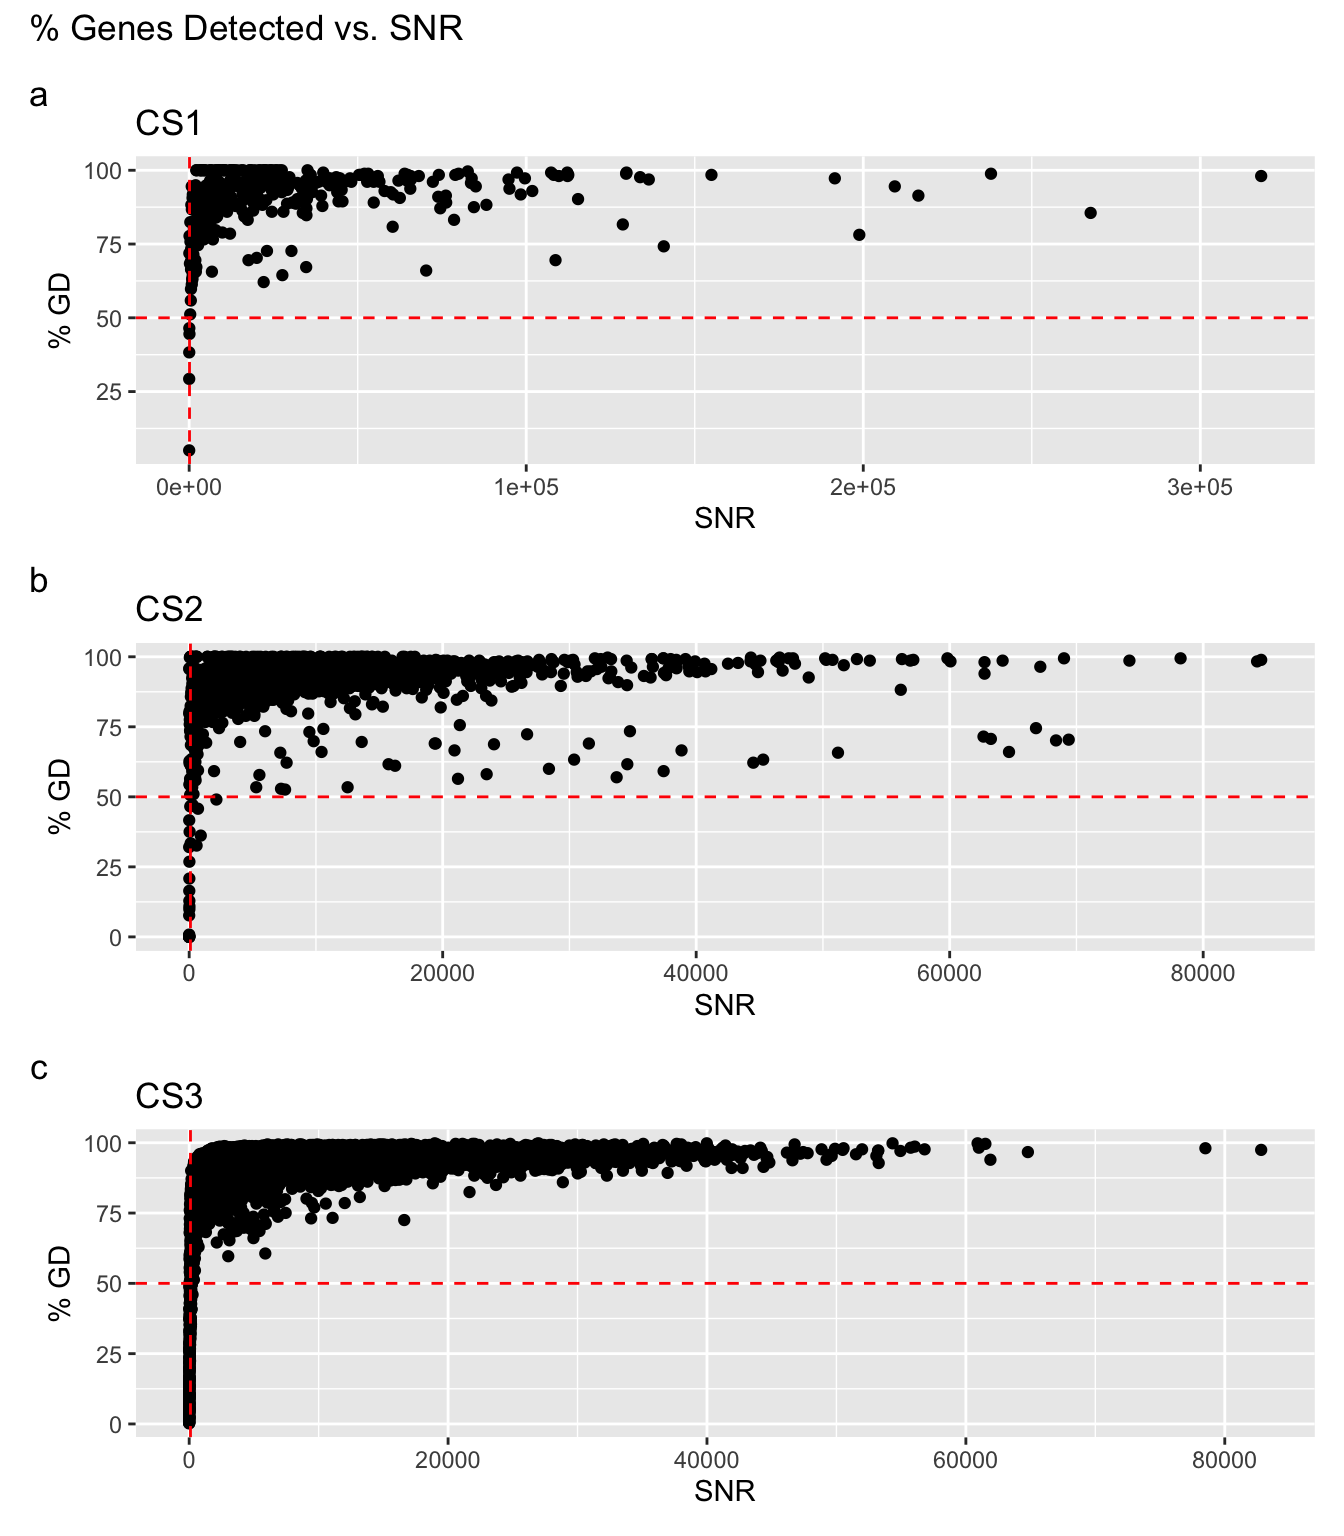
\includegraphics{OV_Histotypes_RSF_files/figure-latex/qc-gd-snr-all-1} 

}

\caption{\% Genes Detected vs. Signal to Noise Ratio}\label{fig:qc-gd-snr-all}
\end{figure}

\begin{figure}[H]

{\centering 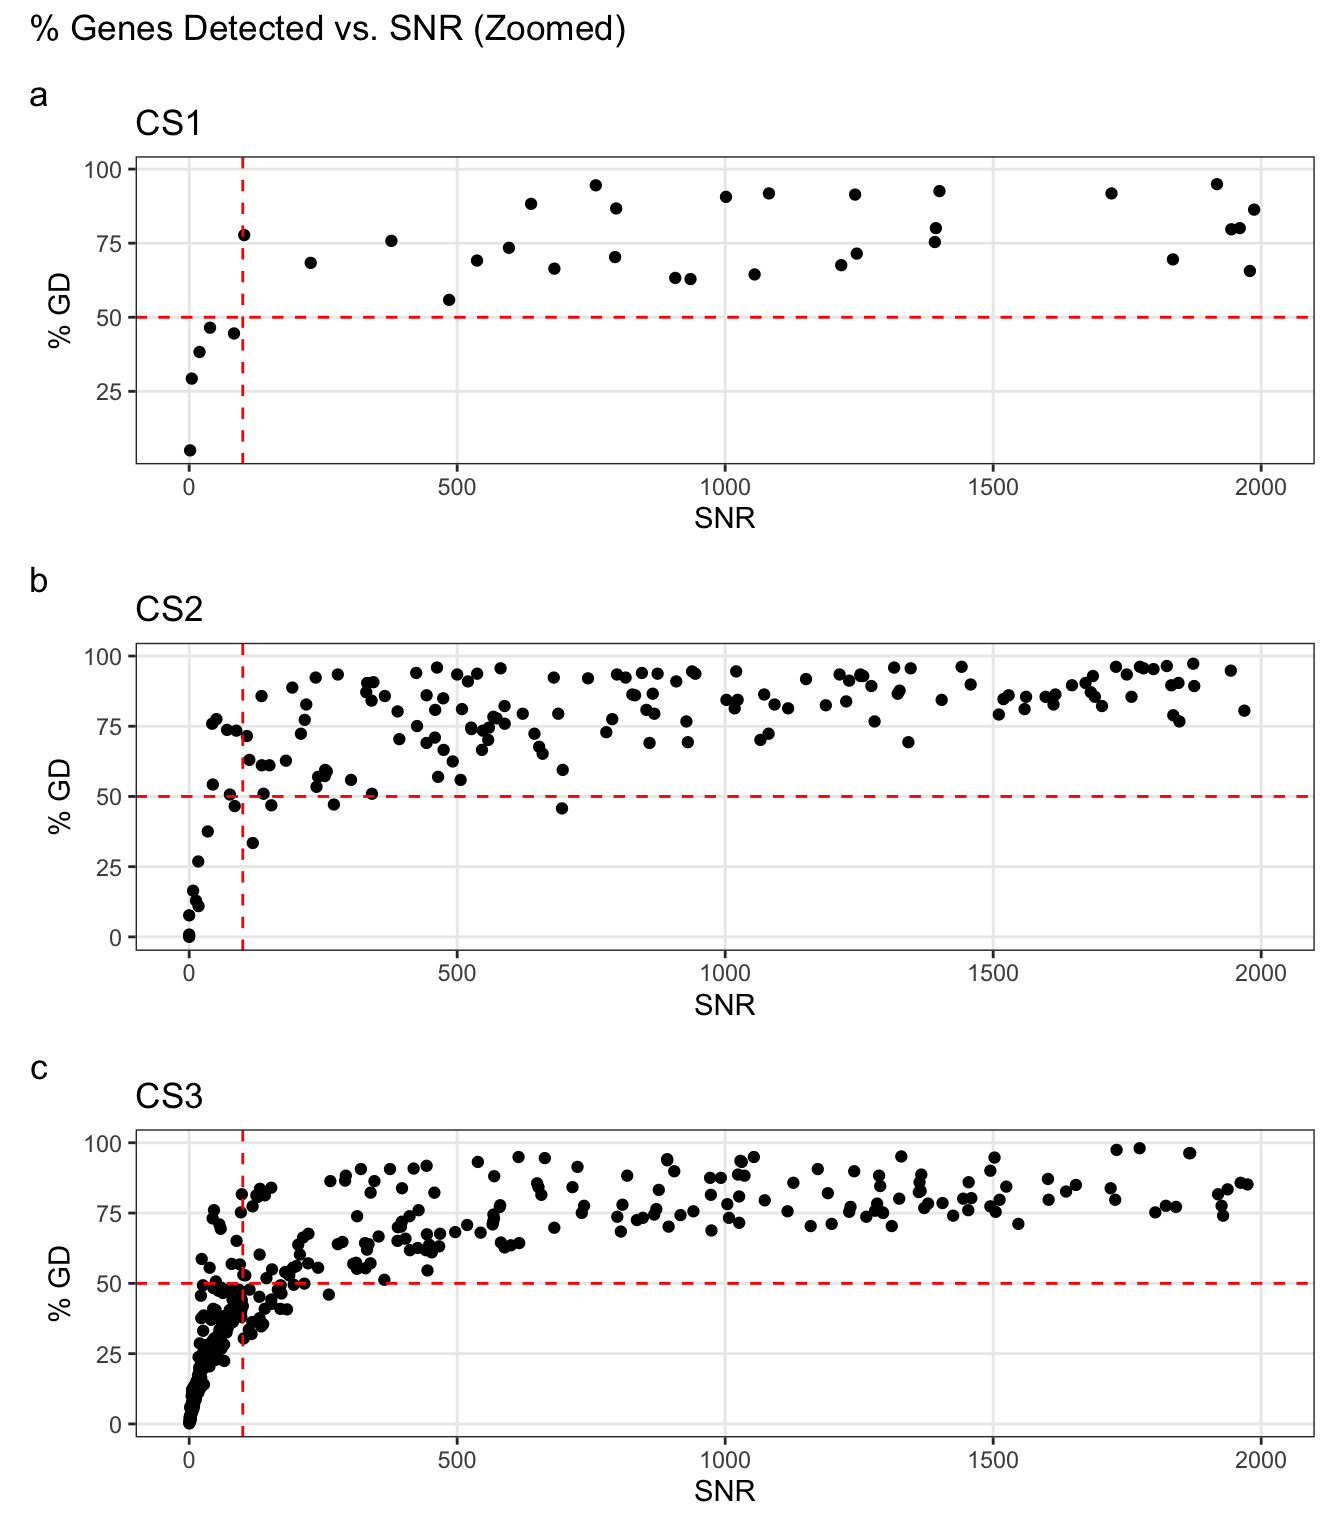
\includegraphics{OV_Histotypes_RSF_files/figure-latex/qc-gd-snr-zoomed-1} 

}

\caption{\% Genes Detected vs. Signal to Noise Ratio (Zoomed)}\label{fig:qc-gd-snr-zoomed}
\end{figure}

\section{Pairwise Gene Expression}\label{pairwise-gene-expression}

\begin{figure}[H]

{\centering 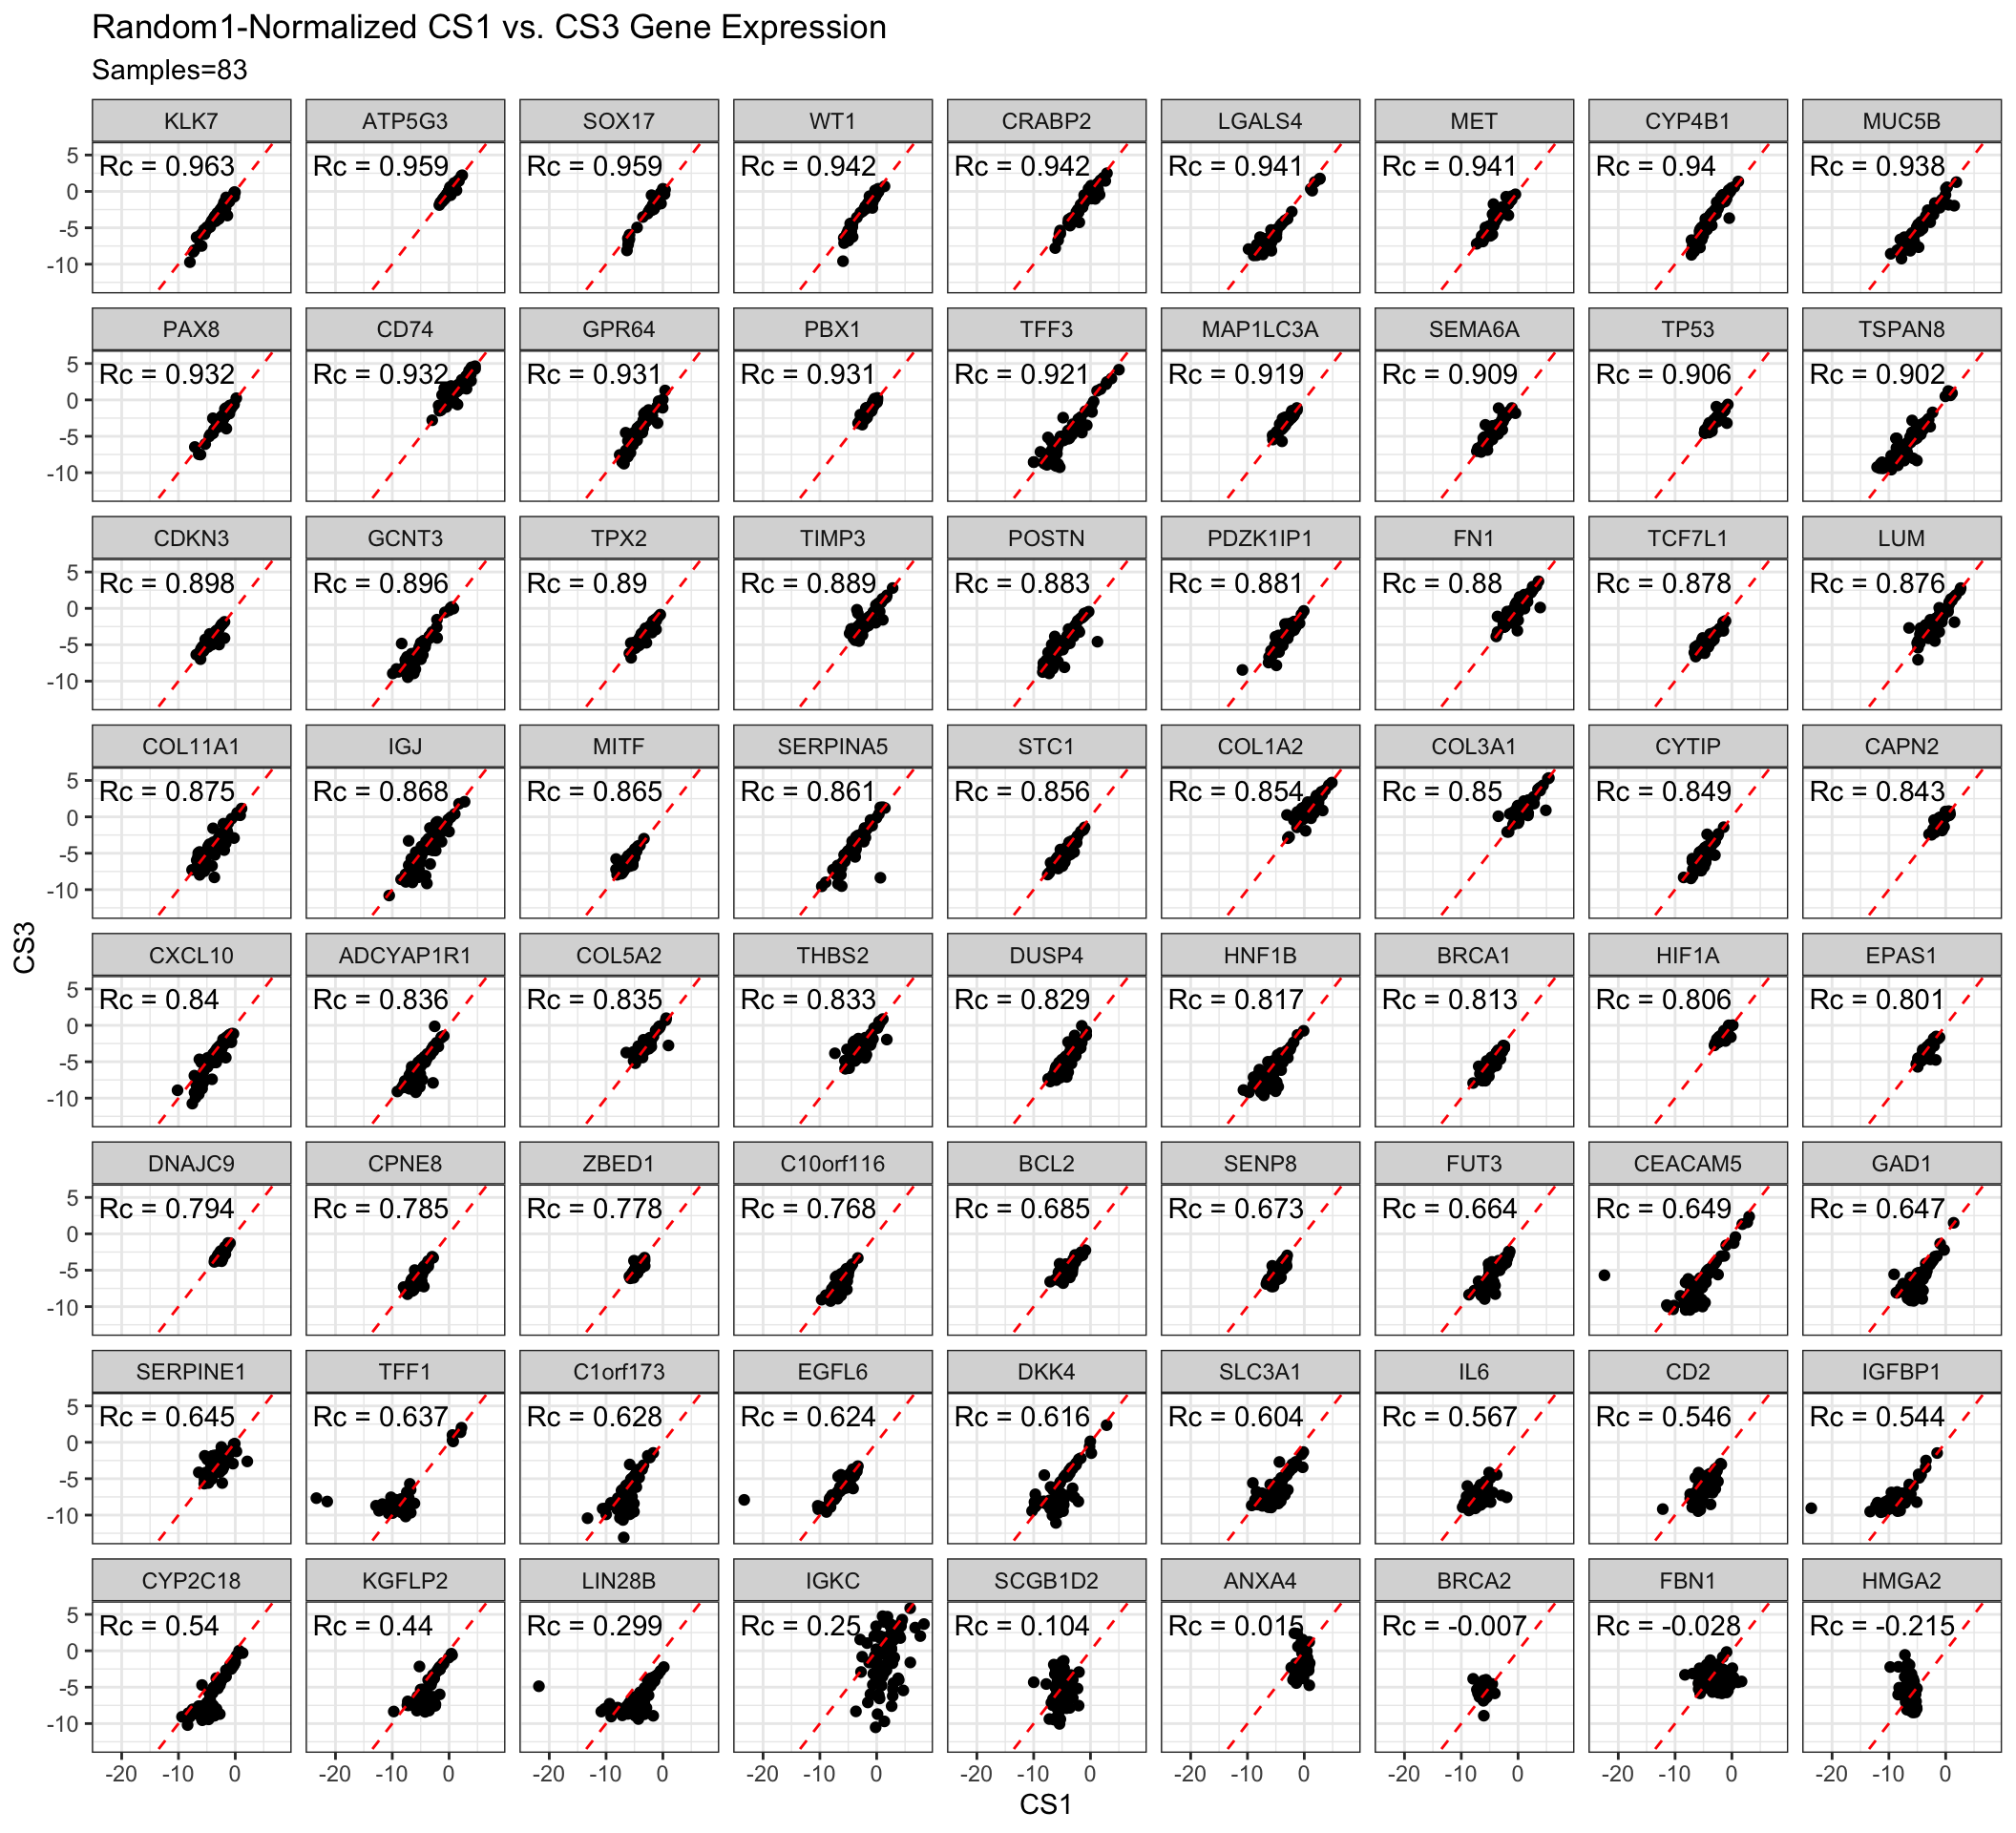
\includegraphics[width=1\linewidth]{OV_Histotypes_RSF_files/figure-latex/genes-cs13-rand1-1} 

}

\caption{Random1-Normalized CS1 vs. CS3 Gene Expression}\label{fig:genes-cs13-rand1}
\end{figure}

\begin{figure}[H]

{\centering 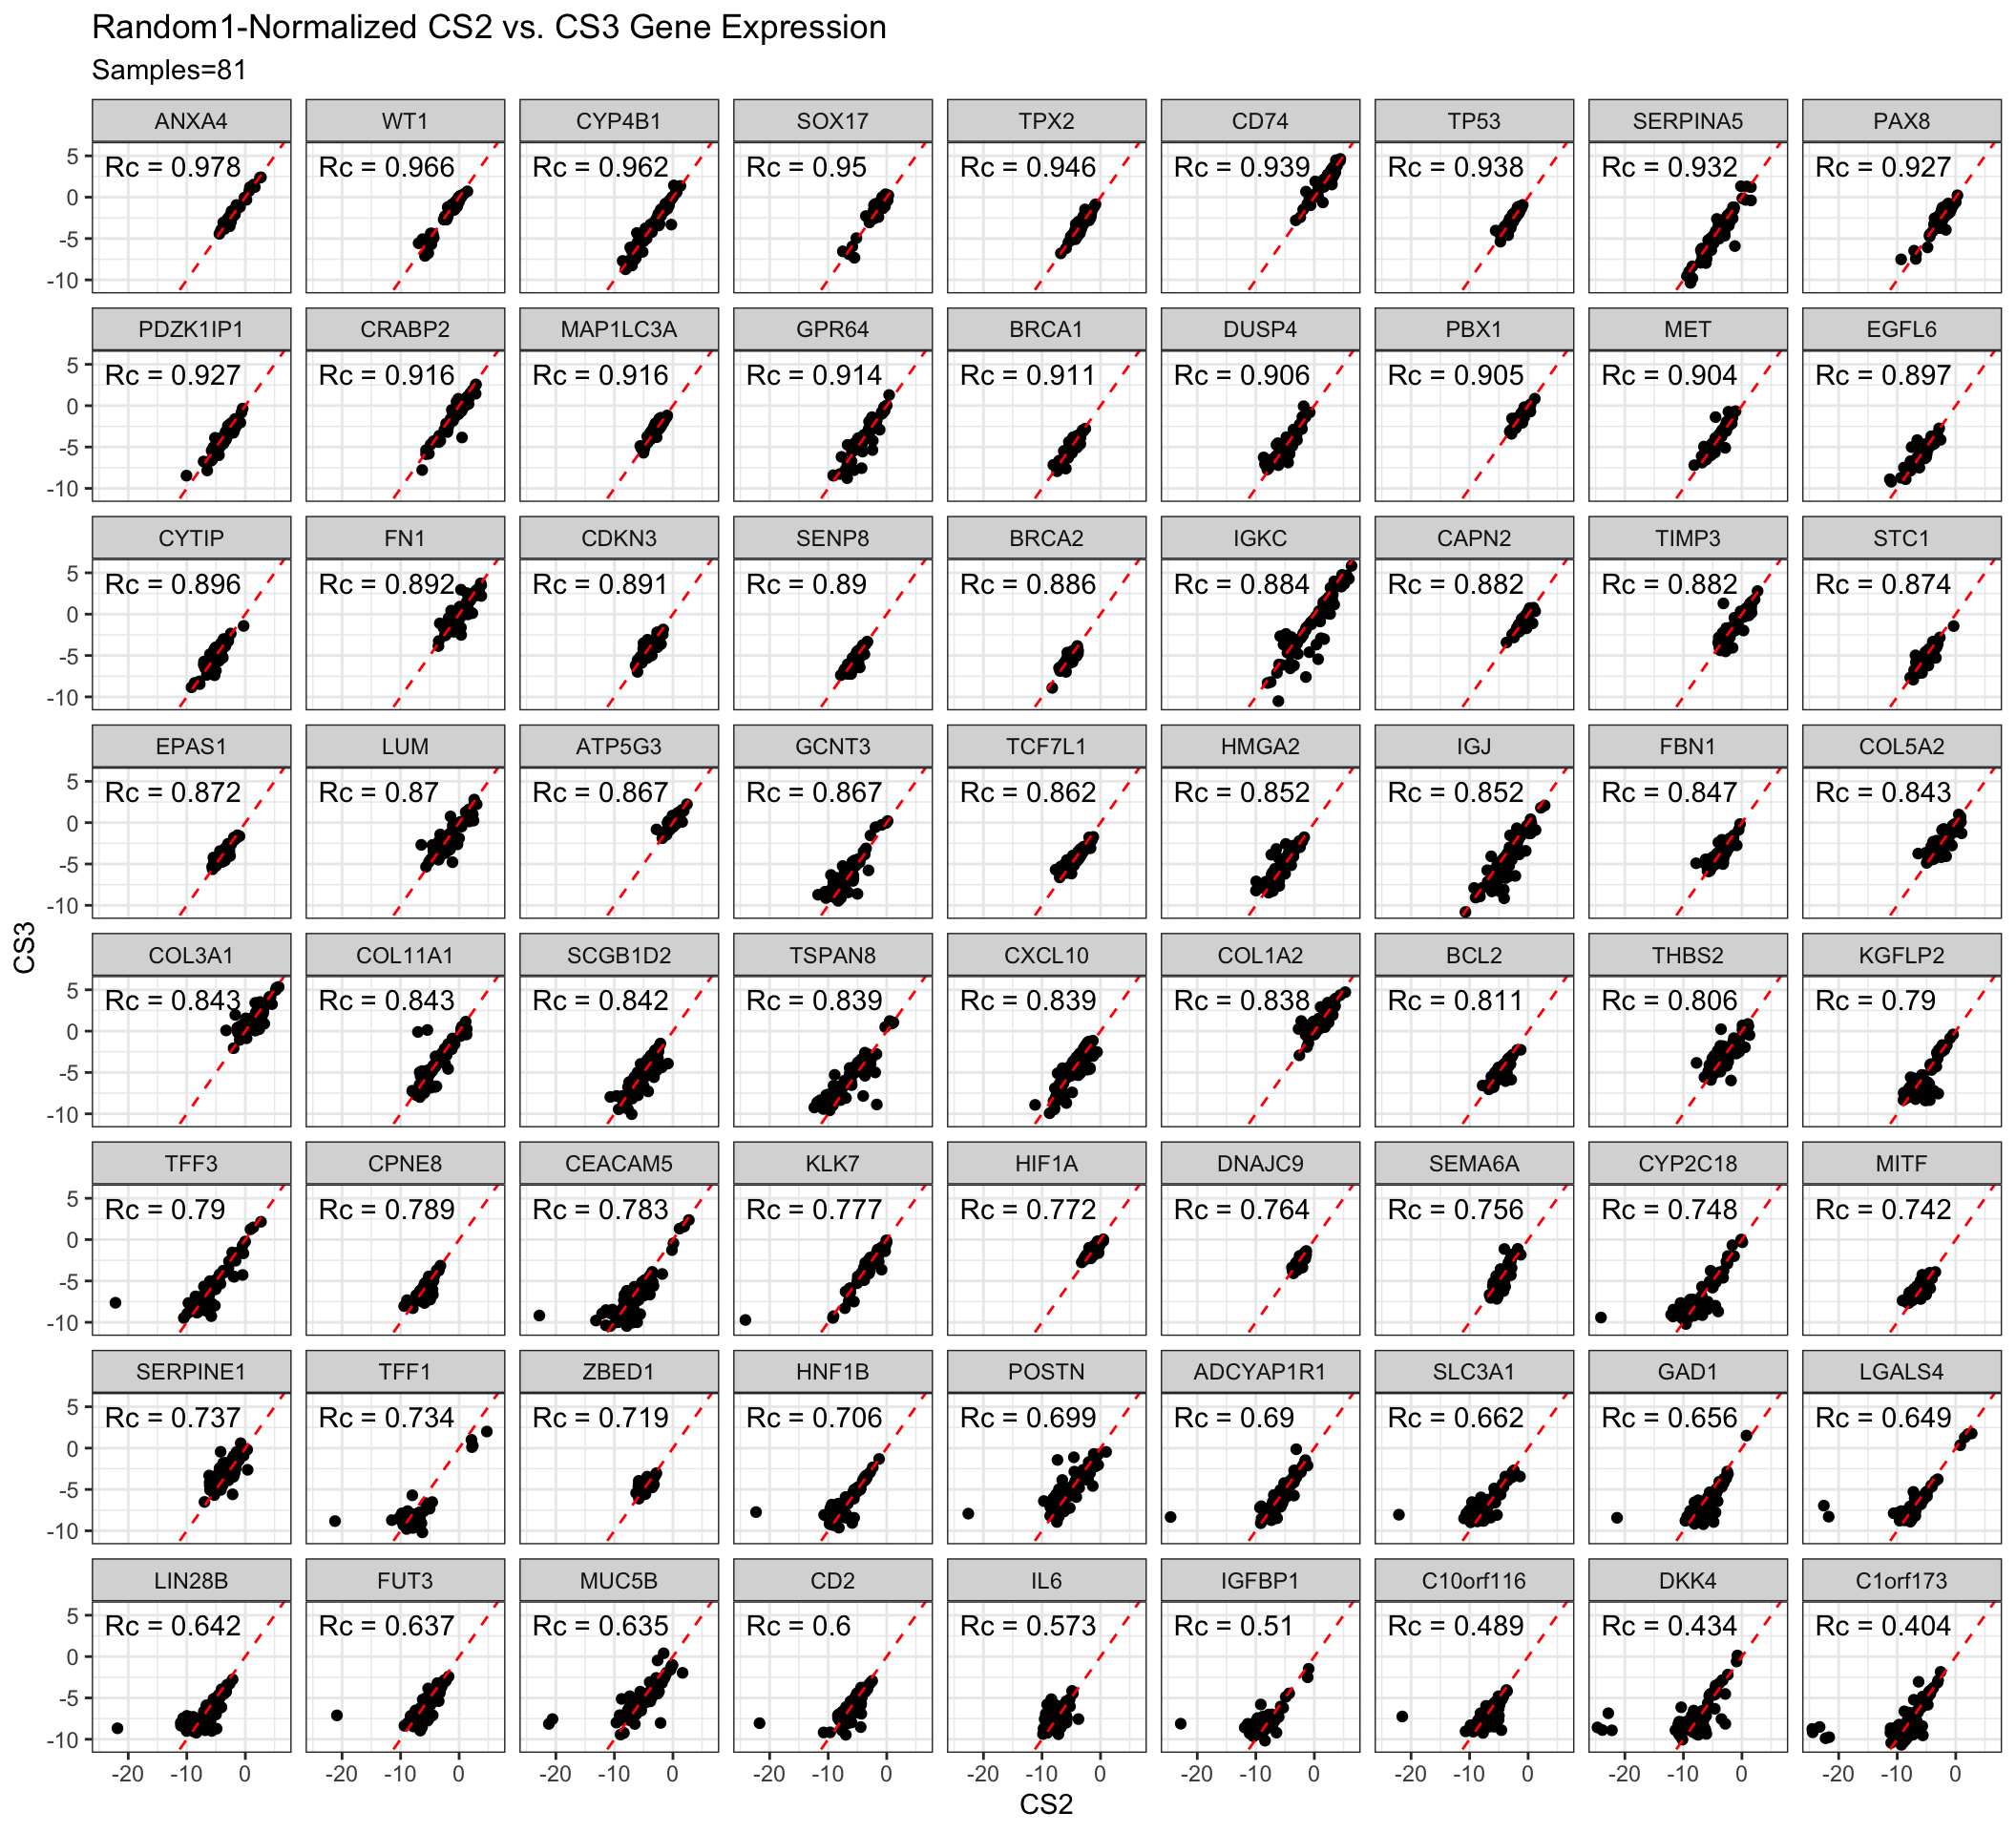
\includegraphics[width=1\linewidth]{OV_Histotypes_RSF_files/figure-latex/genes-cs23-rand1-1} 

}

\caption{Random1-Normalized CS2 vs. CS3 Gene Expression}\label{fig:genes-cs23-rand1}
\end{figure}

\begin{figure}[H]

{\centering 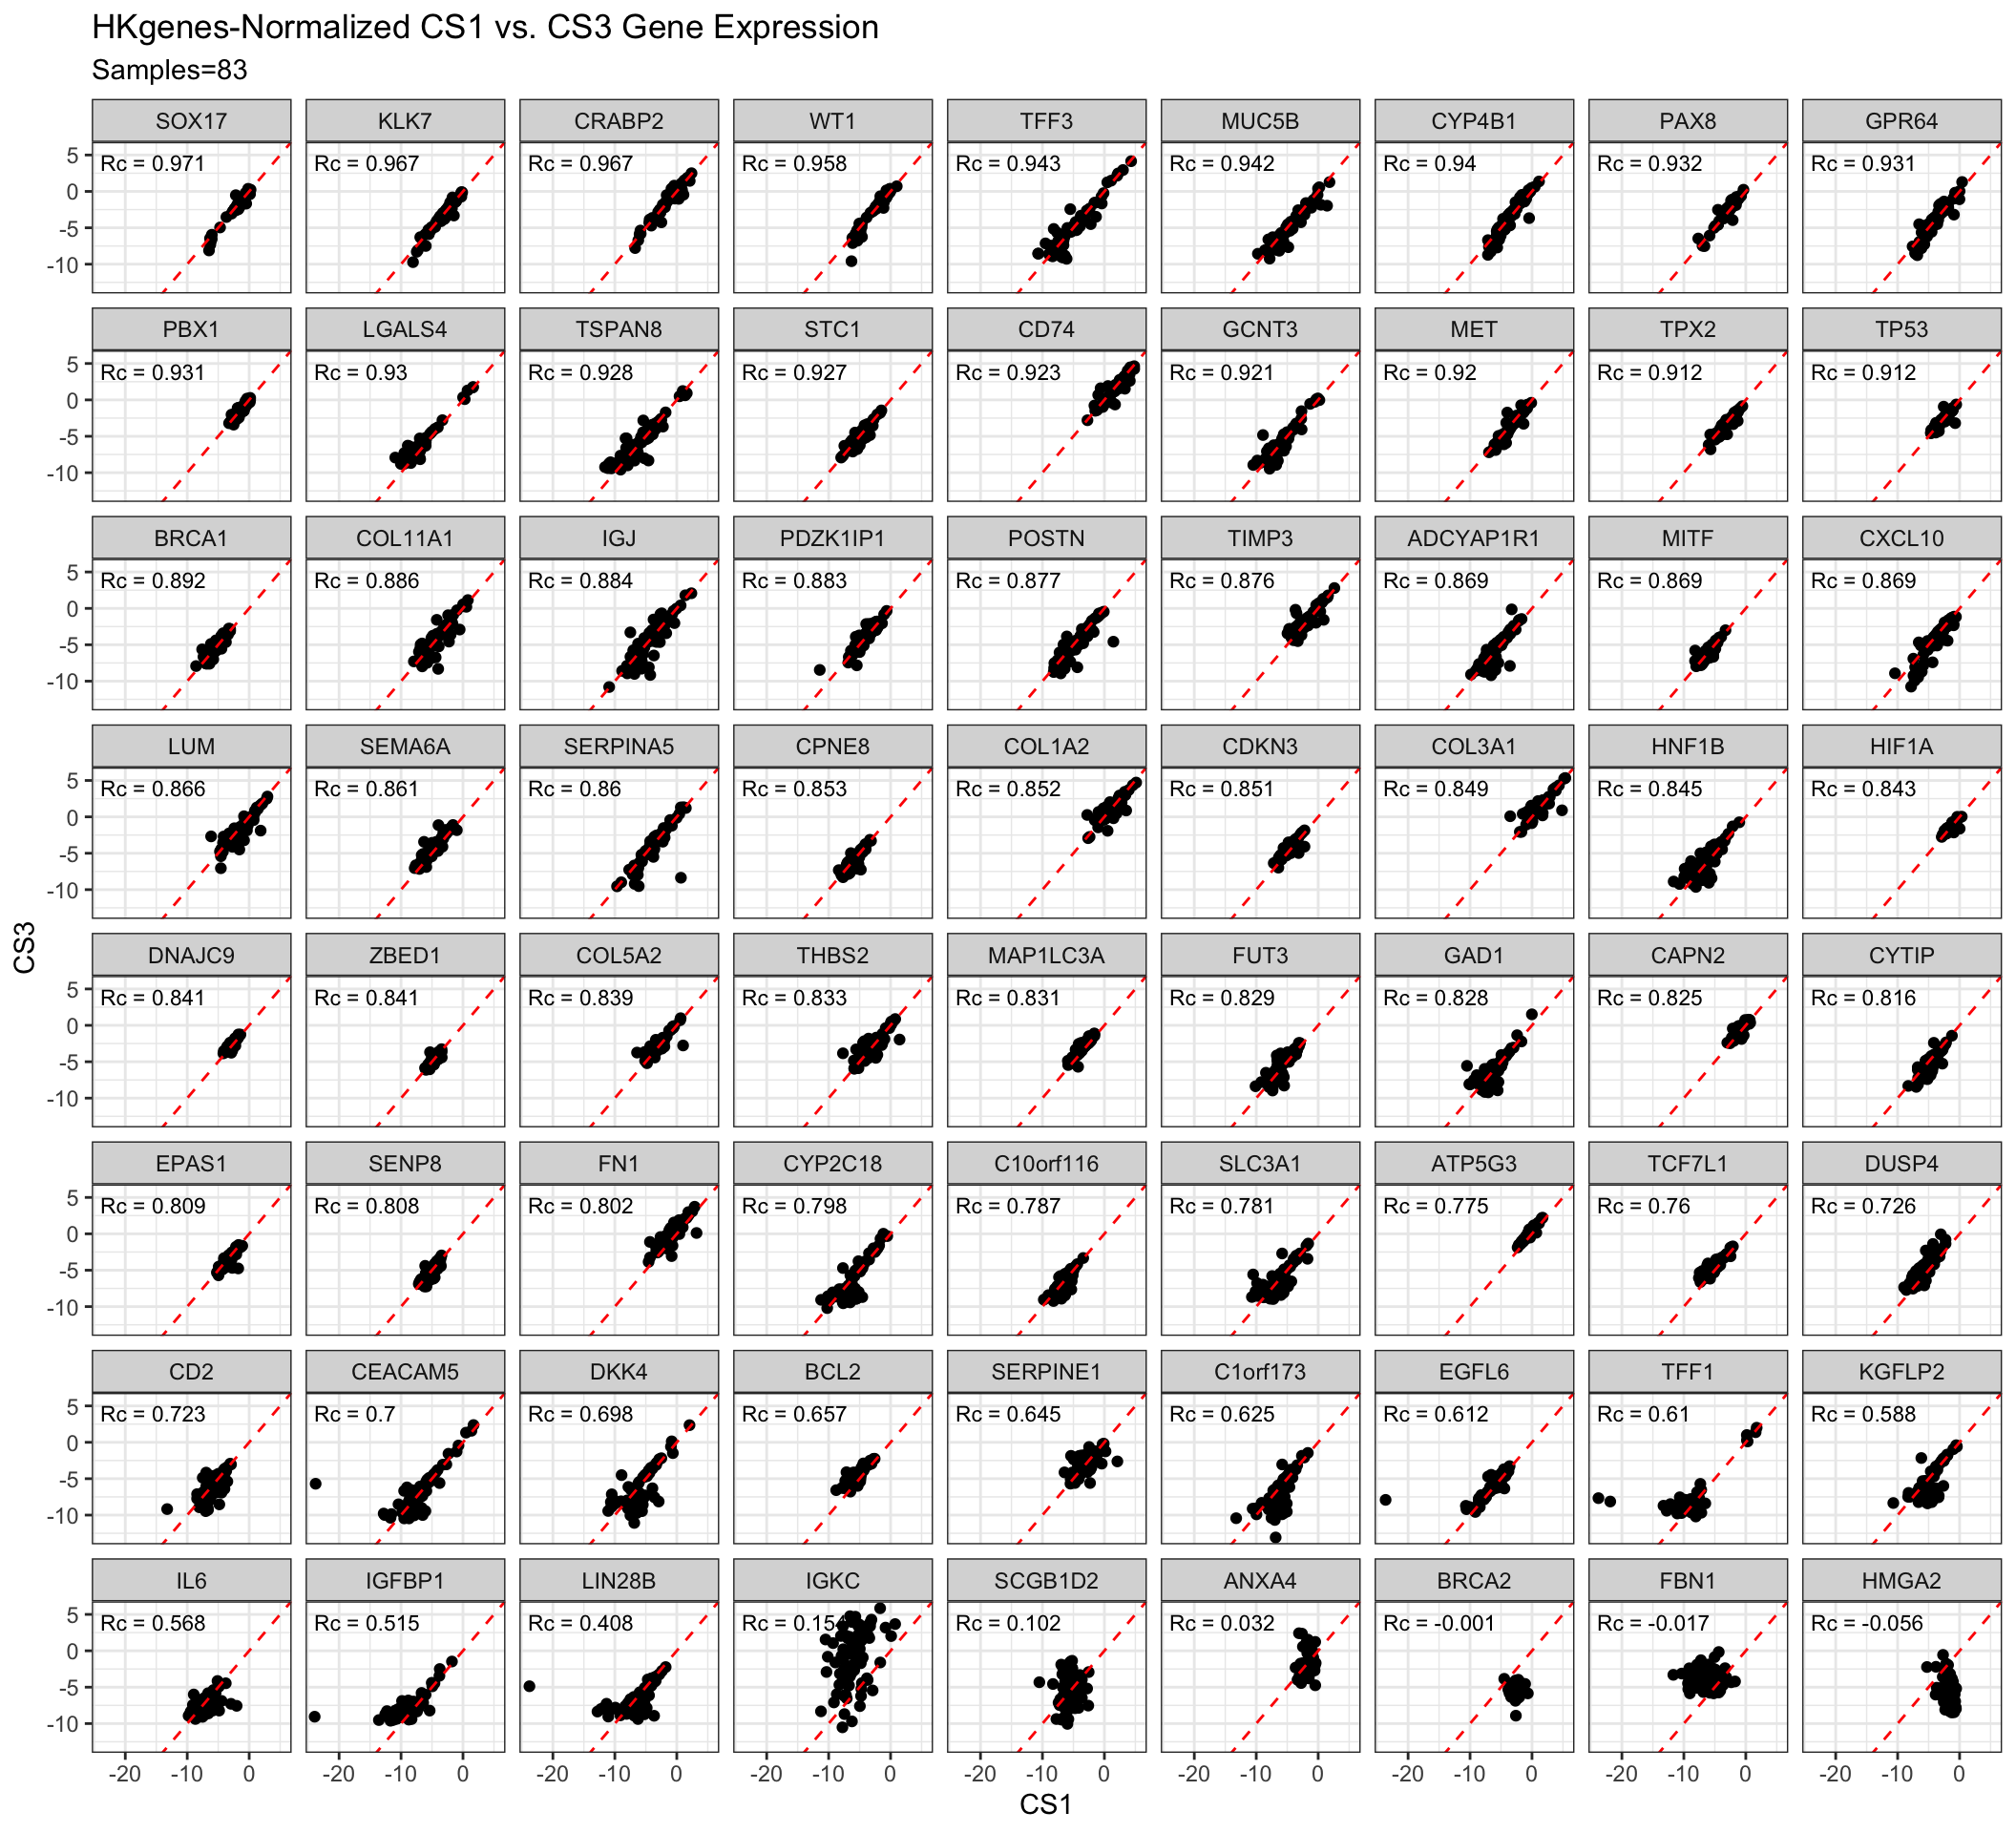
\includegraphics[width=1\linewidth]{OV_Histotypes_RSF_files/figure-latex/genes-cs13-hkgenes-1} 

}

\caption{HKgenes-Normalized CS1 vs. CS3 Gene Expression}\label{fig:genes-cs13-hkgenes}
\end{figure}

\begin{figure}[H]

{\centering 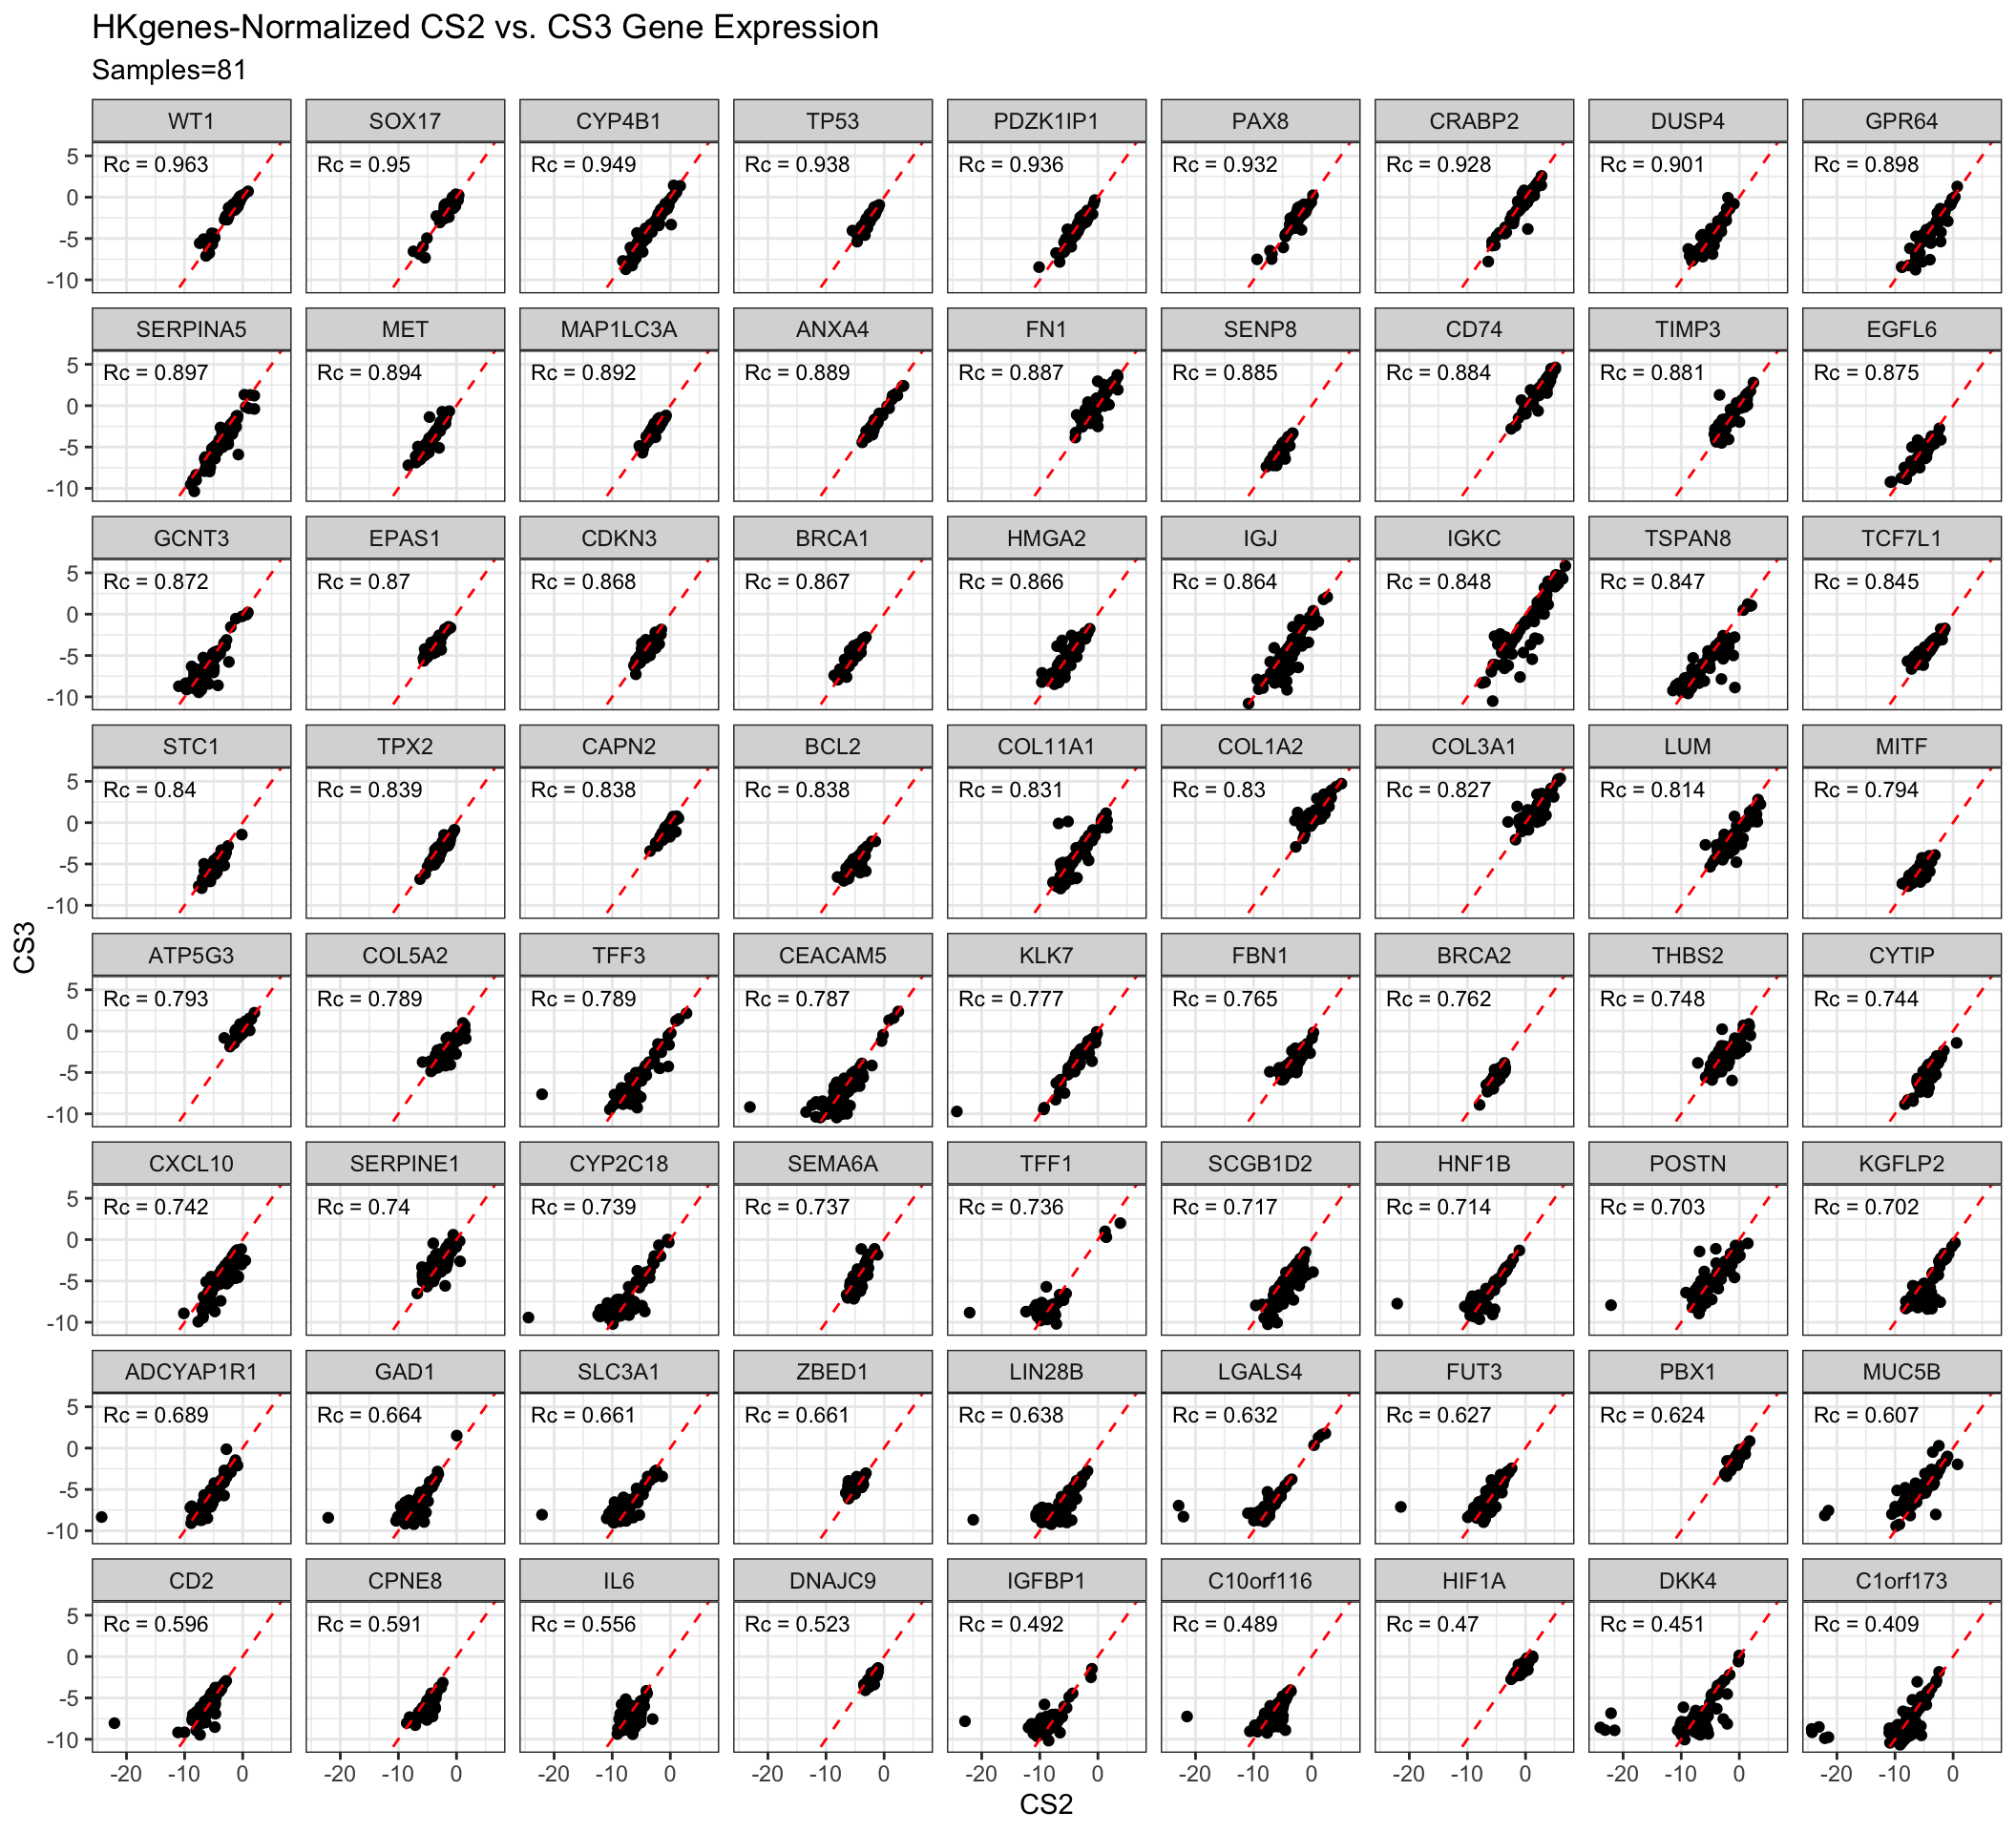
\includegraphics[width=1\linewidth]{OV_Histotypes_RSF_files/figure-latex/genes-cs23-hkgenes-1} 

}

\caption{HKgenes-Normalized CS2 vs. CS3 Gene Expression}\label{fig:genes-cs23-hkgenes}
\end{figure}

\chapter{Results}\label{results}

We summarize cross-validated training performance of class metrics in the training set. The accuracy, F1-score, kappa, and G-mean are the metrics of interest. Workflows are ordered by their mean estimates across the outer folds of the nested CV for each metric.

\section{Training Set}\label{training-set}

\subsection{Accuracy}\label{accuracy-1}

\begin{figure}[H]

{\centering 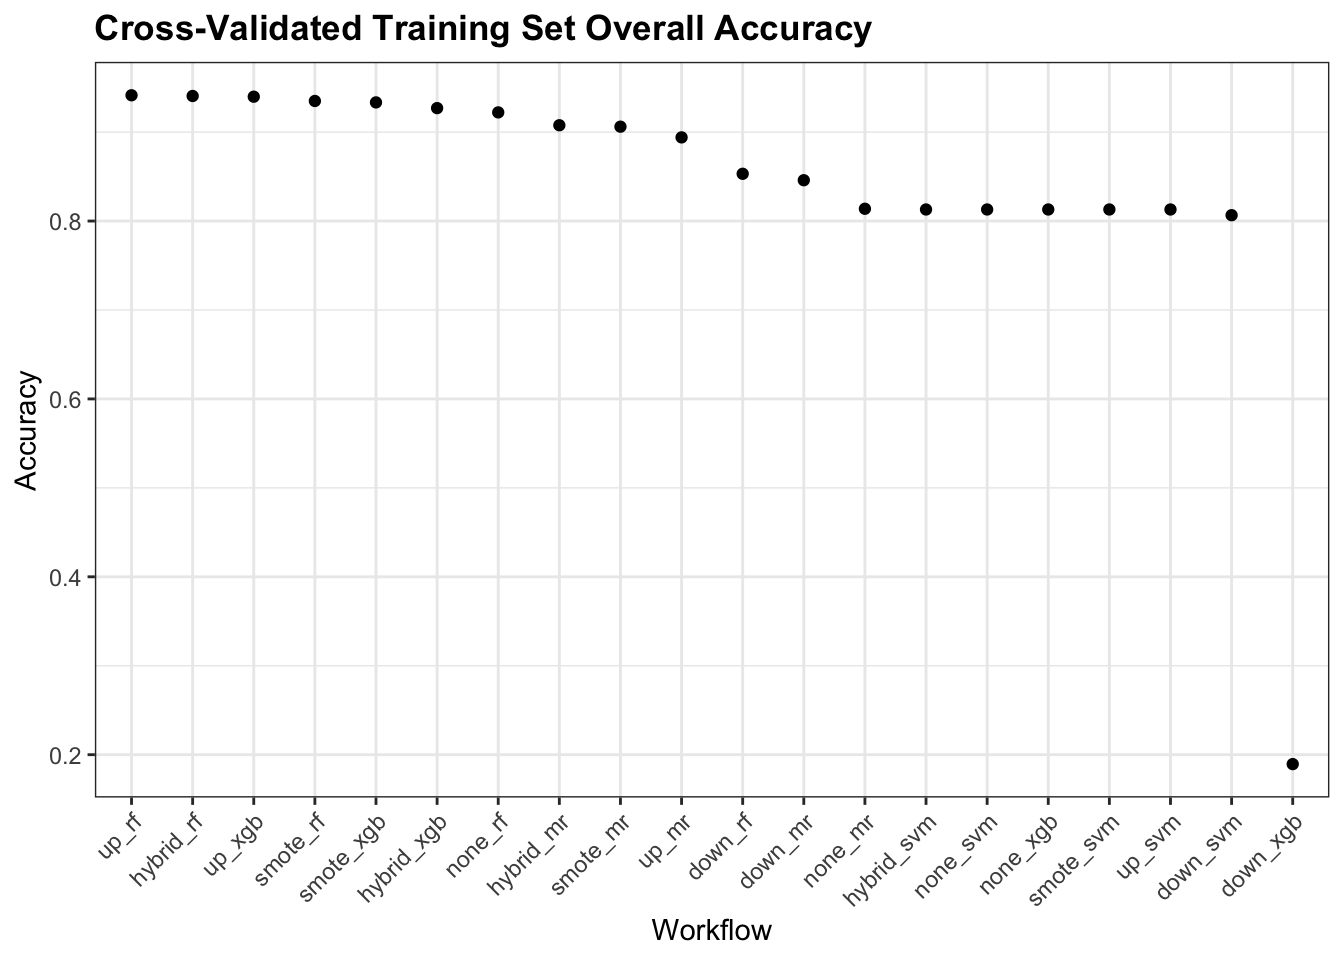
\includegraphics{OV_Histotypes_RSF_files/figure-latex/train-accuracy-1} 

}

\caption{Training Set Mean Accuracy}\label{fig:train-accuracy}
\end{figure}

\begin{table}

\caption{\label{tab:train-accuracy-table}Training Set Mean Accuracy}
\centering
\begin{tabular}[t]{l|l|l|l|l}
\hline
\multicolumn{1}{c|}{ } & \multicolumn{4}{c}{Algorithms} \\
\cline{2-5}
Subsampling & rf & svm & xgb & mr\\
\hline
none & 0.922 & 0.937 & 0.813 & 0.814\\
\hline
down & 0.853 & 0.807 & 0.189 & 0.846\\
\hline
up & \cellcolor[HTML]{90ee90}{0.941} & 0.931 & 0.94 & 0.894\\
\hline
smote & 0.935 & 0.93 & 0.933 & 0.906\\
\hline
hybrid & \cellcolor[HTML]{90ee90}{0.941} & 0.93 & 0.927 & 0.908\\
\hline
\end{tabular}
\end{table}

\begin{figure}[H]

{\centering 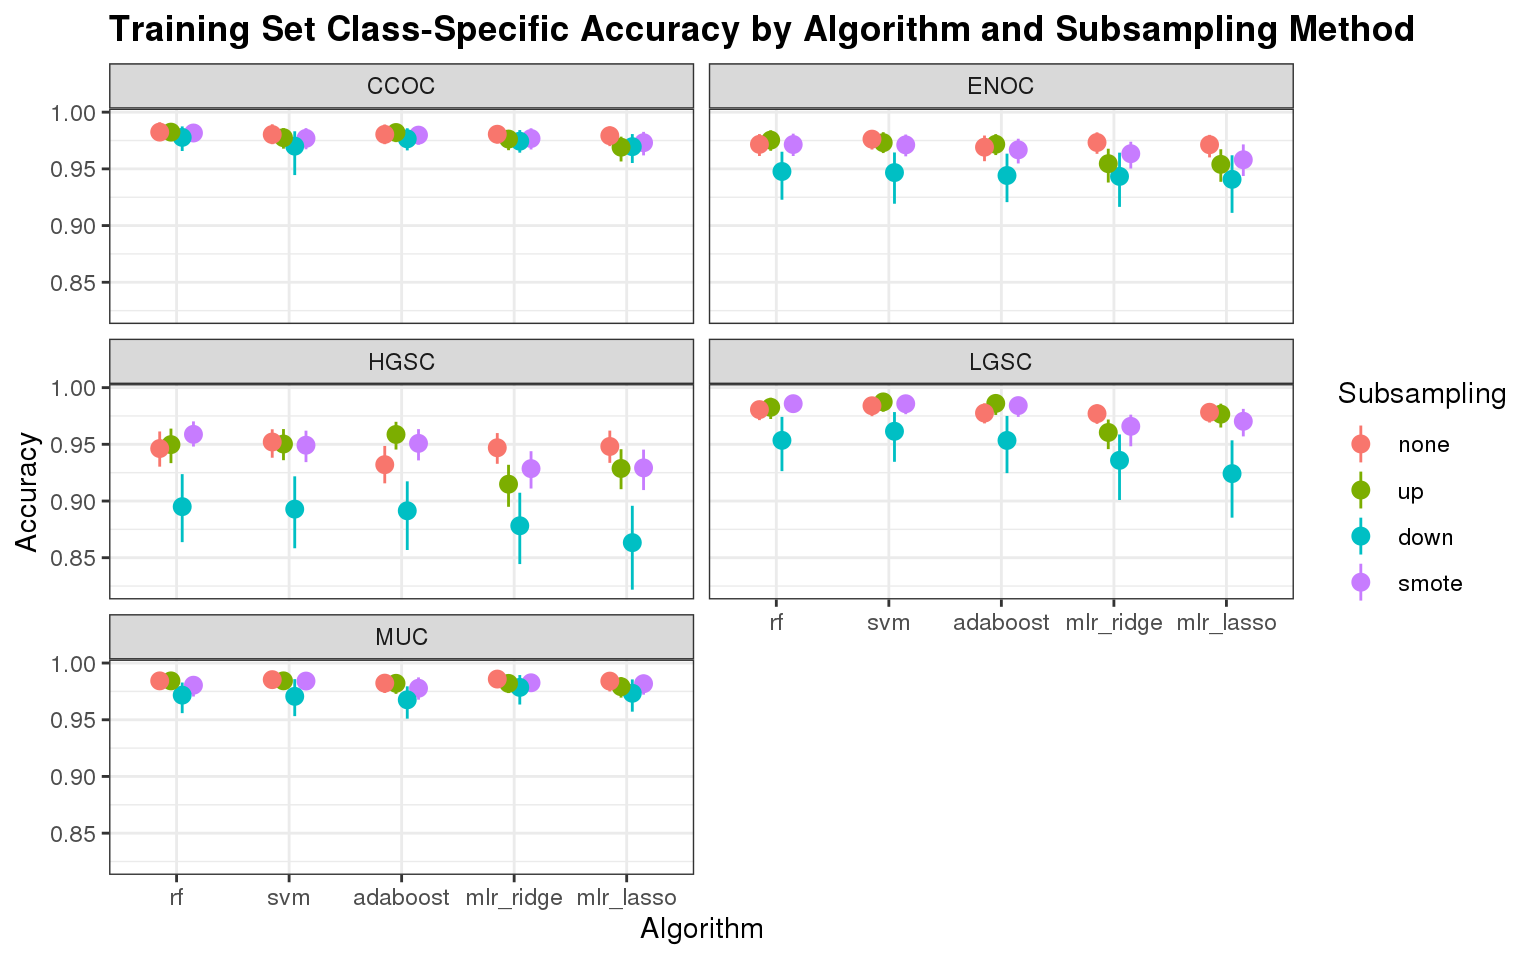
\includegraphics{OV_Histotypes_RSF_files/figure-latex/train-accuracy-class-1} 

}

\caption{Training Set Class-Specific Mean Accuracy}\label{fig:train-accuracy-class}
\end{figure}

\begin{table}

\caption{\label{tab:train-accuracy-class-table}Training Set Class-Specific Mean Accuracy}
\centering
\begin{tabular}[t]{l|l|l|l|l|l}
\hline
\multicolumn{2}{c|}{ } & \multicolumn{4}{c}{Algorithms} \\
\cline{3-6}
Subsampling & Histotype & rf & svm & xgb & mr\\
\hline
 & HGSC & 0.936 & 0.953 & 0.813 & 0.814\\
\cline{2-6}
 & CCOC & 0.982 & 0.983 & 0.935 & 0.936\\
\cline{2-6}
 & ENOC & 0.961 & 0.973 & 0.947 & 0.947\\
\cline{2-6}
 & LGSC & 0.982 & 0.982 & 0.982 & 0.982\\
\cline{2-6}
\multirow{-5}{*}{\raggedright\arraybackslash none} & MUC & 0.983 & 0.983 & 0.949 & 0.949\\
\cline{1-6}
 & HGSC & 0.888 & 0.835 & 0.31 & 0.876\\
\cline{2-6}
 & CCOC & 0.973 & 0.969 & 0.935 & 0.974\\
\cline{2-6}
 & ENOC & 0.96 & 0.929 & 0.947 & 0.945\\
\cline{2-6}
 & LGSC & 0.927 & 0.904 & 0.596 & 0.926\\
\cline{2-6}
\multirow{-5}{*}{\raggedright\arraybackslash down} & MUC & 0.959 & 0.976 & 0.59 & 0.971\\
\cline{1-6}
 & HGSC & 0.96 & 0.955 & 0.961 & 0.924\\
\cline{2-6}
 & CCOC & 0.984 & 0.978 & 0.984 & 0.975\\
\cline{2-6}
 & ENOC & 0.975 & 0.964 & 0.972 & 0.954\\
\cline{2-6}
 & LGSC & 0.981 & 0.982 & 0.982 & 0.961\\
\cline{2-6}
\multirow{-5}{*}{\raggedright\arraybackslash up} & MUC & 0.983 & 0.982 & 0.981 & 0.974\\
\cline{1-6}
 & HGSC & 0.957 & 0.955 & 0.96 & 0.932\\
\cline{2-6}
 & CCOC & 0.979 & 0.975 & 0.981 & 0.978\\
\cline{2-6}
 & ENOC & 0.97 & 0.961 & 0.967 & 0.959\\
\cline{2-6}
 & LGSC & 0.981 & \cellcolor[HTML]{90ee90}{0.985} & 0.979 & 0.966\\
\cline{2-6}
\multirow{-5}{*}{\raggedright\arraybackslash smote} & MUC & 0.982 & 0.984 & 0.98 & 0.978\\
\cline{1-6}
 & HGSC & 0.962 & 0.957 & 0.952 & 0.939\\
\cline{2-6}
 & CCOC & 0.984 & 0.979 & 0.98 & 0.976\\
\cline{2-6}
 & ENOC & 0.973 & 0.962 & 0.966 & 0.957\\
\cline{2-6}
 & LGSC & 0.982 & 0.982 & 0.978 & 0.969\\
\cline{2-6}
\multirow{-5}{*}{\raggedright\arraybackslash hybrid} & MUC & 0.98 & 0.981 & 0.978 & 0.975\\
\hline
\end{tabular}
\end{table}

\subsection{Sensitivity}\label{sensitivity-1}

\begin{figure}[H]

{\centering 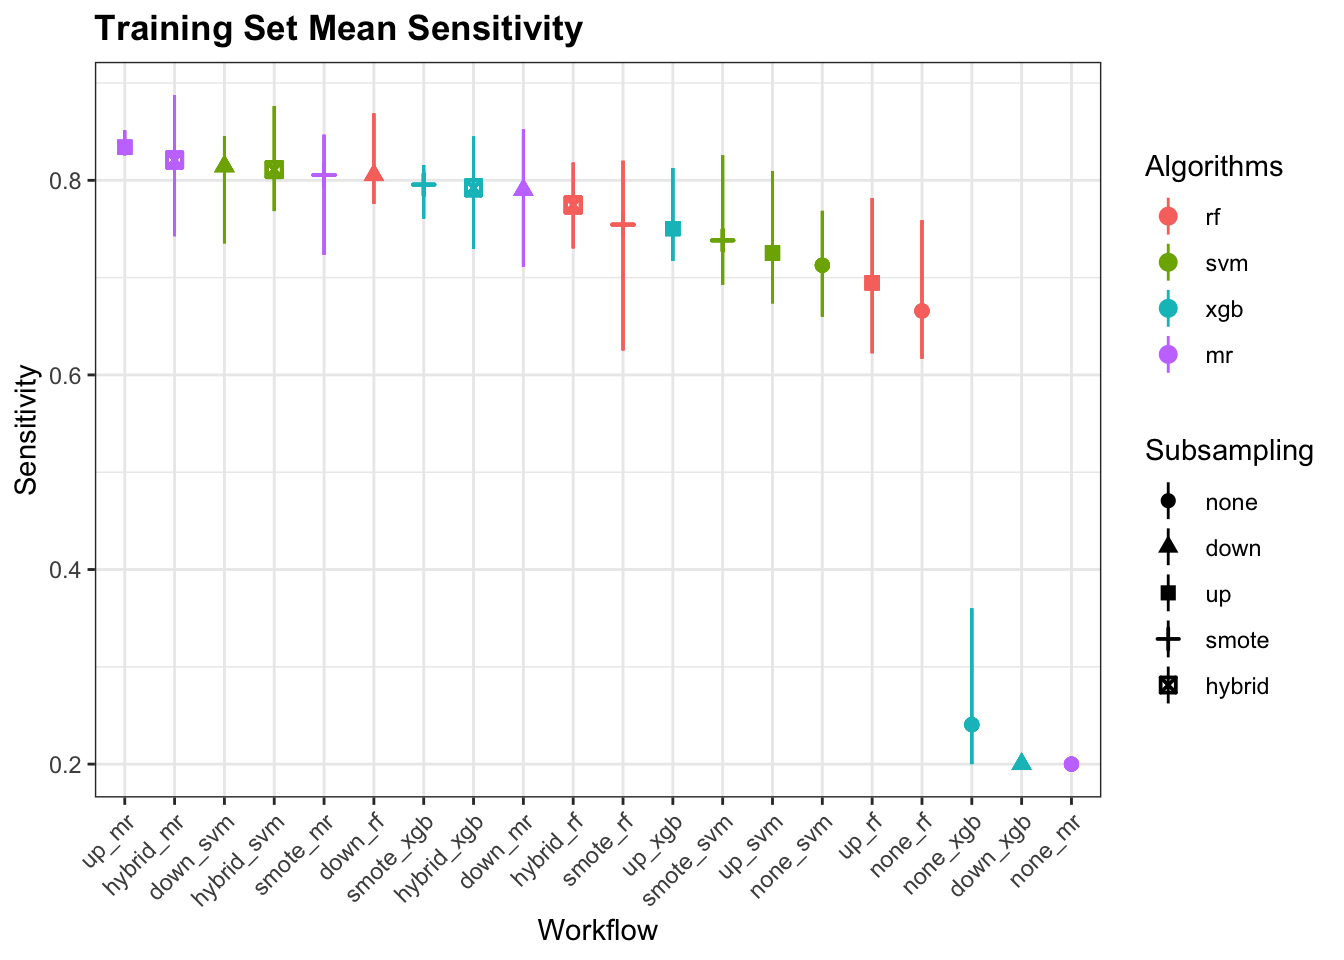
\includegraphics{OV_Histotypes_RSF_files/figure-latex/train-sens-1} 

}

\caption{Training Set Mean Sensitivity}\label{fig:train-sens}
\end{figure}

\begin{table}

\caption{\label{tab:train-sens-table}Training Set Mean Sensitivity}
\centering
\begin{tabular}[t]{l|l|l|l|l}
\hline
\multicolumn{1}{c|}{ } & \multicolumn{4}{c}{Algorithms} \\
\cline{2-5}
Subsampling & rf & svm & xgb & mr\\
\hline
none & 0.602 & 0.669 & 0.2 & 0.203\\
\hline
down & 0.805 & \cellcolor[HTML]{90ee90}{0.838} & 0.2 & 0.829\\
\hline
up & 0.697 & 0.714 & 0.737 & 0.82\\
\hline
smote & 0.708 & 0.682 & 0.765 & 0.802\\
\hline
hybrid & 0.771 & 0.758 & 0.754 & 0.796\\
\hline
\end{tabular}
\end{table}

\begin{figure}[H]

{\centering 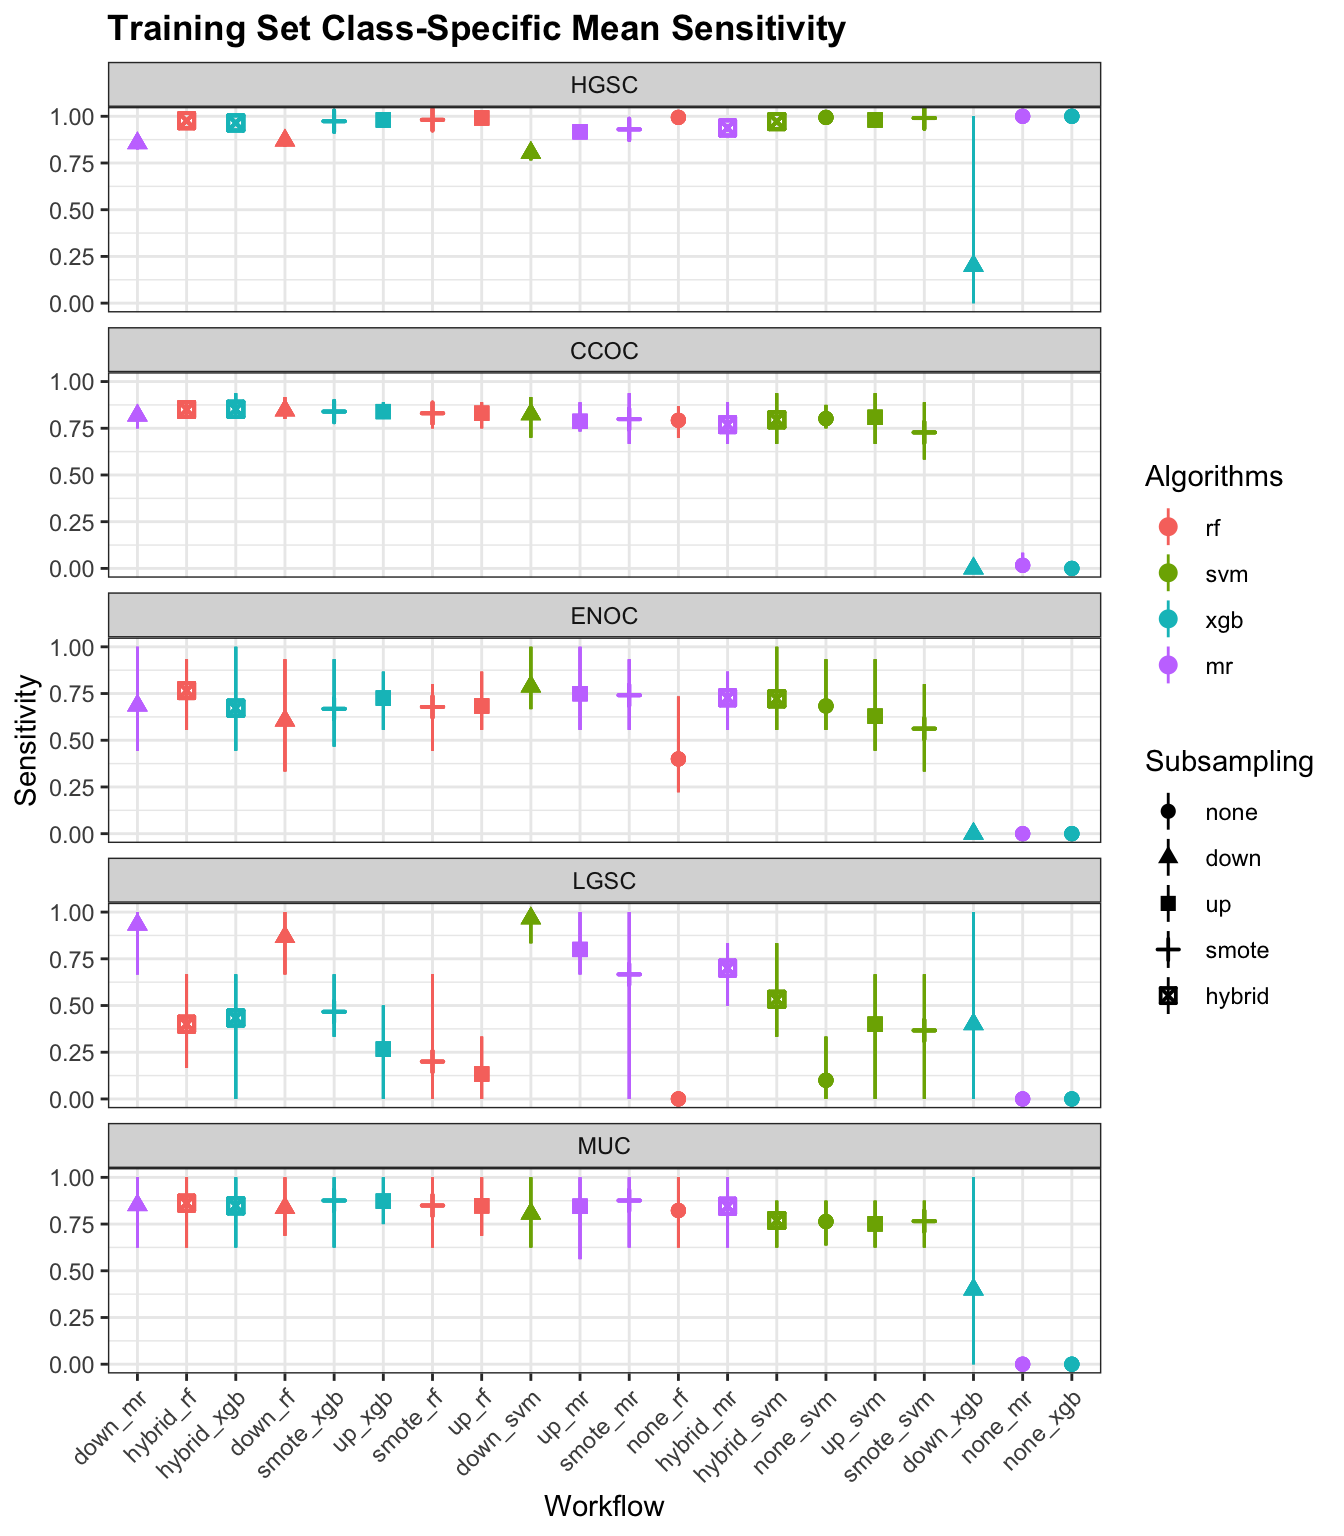
\includegraphics{OV_Histotypes_RSF_files/figure-latex/train-sens-class-1} 

}

\caption{Training Set Class-Specific Mean Sensitivity}\label{fig:train-sens-class}
\end{figure}

\begin{table}

\caption{\label{tab:train-sens-class-table}Cross-Validated Training Set Class-Specific Mean Sensitivity}
\centering
\begin{tabular}[t]{l|l|l|l|l|l}
\hline
\multicolumn{2}{c|}{ } & \multicolumn{4}{c}{Algorithms} \\
\cline{3-6}
Subsampling & Histotype & rf & svm & xgb & mr\\
\hline
 & HGSC & 0.994 & 0.994 & \cellcolor[HTML]{90ee90}{1} & \cellcolor[HTML]{90ee90}{1}\\
\cline{2-6}
 & CCOC & 0.792 & 0.802 & 0 & 0.017\\
\cline{2-6}
 & ENOC & 0.4 & 0.683 & 0 & 0\\
\cline{2-6}
 & LGSC & 0 & 0.1 & 0 & 0\\
\cline{2-6}
\multirow{-5}{*}{\raggedright\arraybackslash none} & MUC & 0.823 & 0.764 & 0 & 0\\
\cline{1-6}
 & HGSC & 0.871 & 0.805 & 0.2 & 0.856\\
\cline{2-6}
 & CCOC & 0.846 & 0.825 & 0 & 0.818\\
\cline{2-6}
 & ENOC & 0.606 & 0.788 & 0 & 0.686\\
\cline{2-6}
 & LGSC & 0.867 & 0.967 & 0.4 & 0.933\\
\cline{2-6}
\multirow{-5}{*}{\raggedright\arraybackslash down} & MUC & 0.837 & 0.806 & 0.4 & 0.851\\
\cline{1-6}
 & HGSC & 0.991 & 0.98 & 0.98 & 0.917\\
\cline{2-6}
 & CCOC & 0.83 & 0.809 & 0.839 & 0.787\\
\cline{2-6}
 & ENOC & 0.683 & 0.629 & 0.726 & 0.749\\
\cline{2-6}
 & LGSC & 0.133 & 0.4 & 0.267 & 0.8\\
\cline{2-6}
\multirow{-5}{*}{\raggedright\arraybackslash up} & MUC & 0.848 & 0.751 & 0.873 & 0.845\\
\cline{1-6}
 & HGSC & 0.981 & 0.99 & 0.973 & 0.93\\
\cline{2-6}
 & CCOC & 0.83 & 0.728 & 0.839 & 0.799\\
\cline{2-6}
 & ENOC & 0.679 & 0.562 & 0.668 & 0.741\\
\cline{2-6}
 & LGSC & 0.2 & 0.367 & 0.467 & 0.667\\
\cline{2-6}
\multirow{-5}{*}{\raggedright\arraybackslash smote} & MUC & 0.849 & 0.765 & 0.876 & 0.876\\
\cline{1-6}
 & HGSC & 0.976 & 0.971 & 0.964 & 0.938\\
\cline{2-6}
 & CCOC & 0.85 & 0.795 & 0.852 & 0.769\\
\cline{2-6}
 & ENOC & 0.766 & 0.722 & 0.672 & 0.727\\
\cline{2-6}
 & LGSC & 0.4 & 0.533 & 0.433 & 0.7\\
\cline{2-6}
\multirow{-5}{*}{\raggedright\arraybackslash hybrid} & MUC & 0.862 & 0.769 & 0.848 & 0.845\\
\hline
\end{tabular}
\end{table}

\subsection{Specificity}\label{specificity-1}

\begin{figure}[H]

{\centering 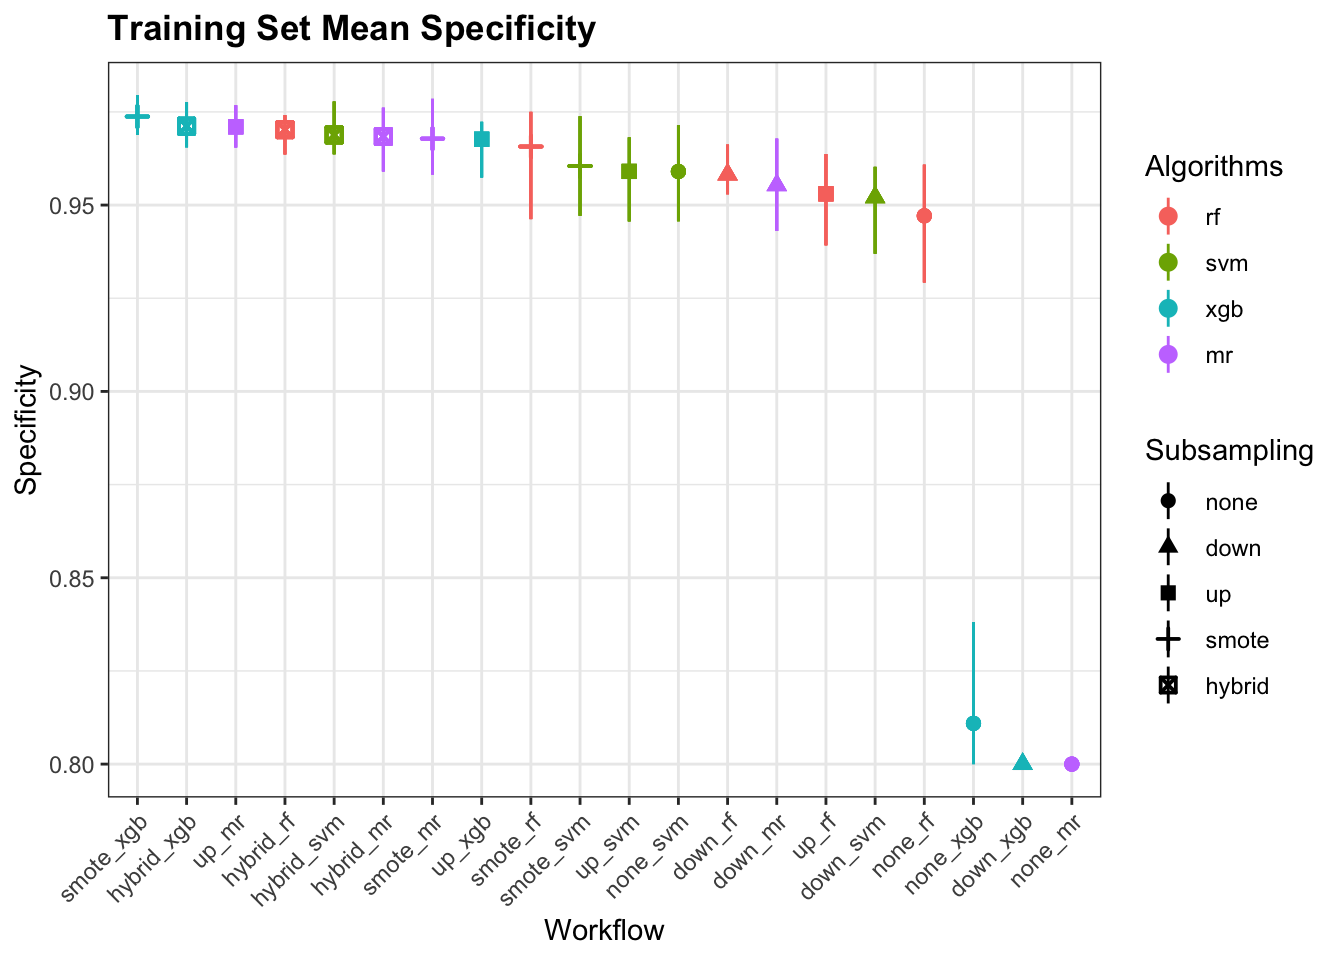
\includegraphics{OV_Histotypes_RSF_files/figure-latex/train-spec-1} 

}

\caption{Training Set Mean Specificity}\label{fig:train-spec}
\end{figure}

\begin{table}

\caption{\label{tab:train-spec-table}Training Set Mean Specificity}
\centering
\begin{tabular}[t]{l|l|l|l|l}
\hline
\multicolumn{1}{c|}{ } & \multicolumn{4}{c}{Algorithms} \\
\cline{2-5}
Subsampling & rf & svm & xgb & mr\\
\hline
none & 0.933 & 0.951 & 0.8 & 0.801\\
\hline
down & 0.963 & 0.955 & 0.8 & 0.962\\
\hline
up & 0.959 & 0.961 & 0.968 & 0.97\\
\hline
smote & 0.963 & 0.954 & 0.97 & 0.971\\
\hline
hybrid & \cellcolor[HTML]{90ee90}{0.972} & 0.968 & 0.968 & \cellcolor[HTML]{90ee90}{0.972}\\
\hline
\end{tabular}
\end{table}

\begin{figure}[H]

{\centering 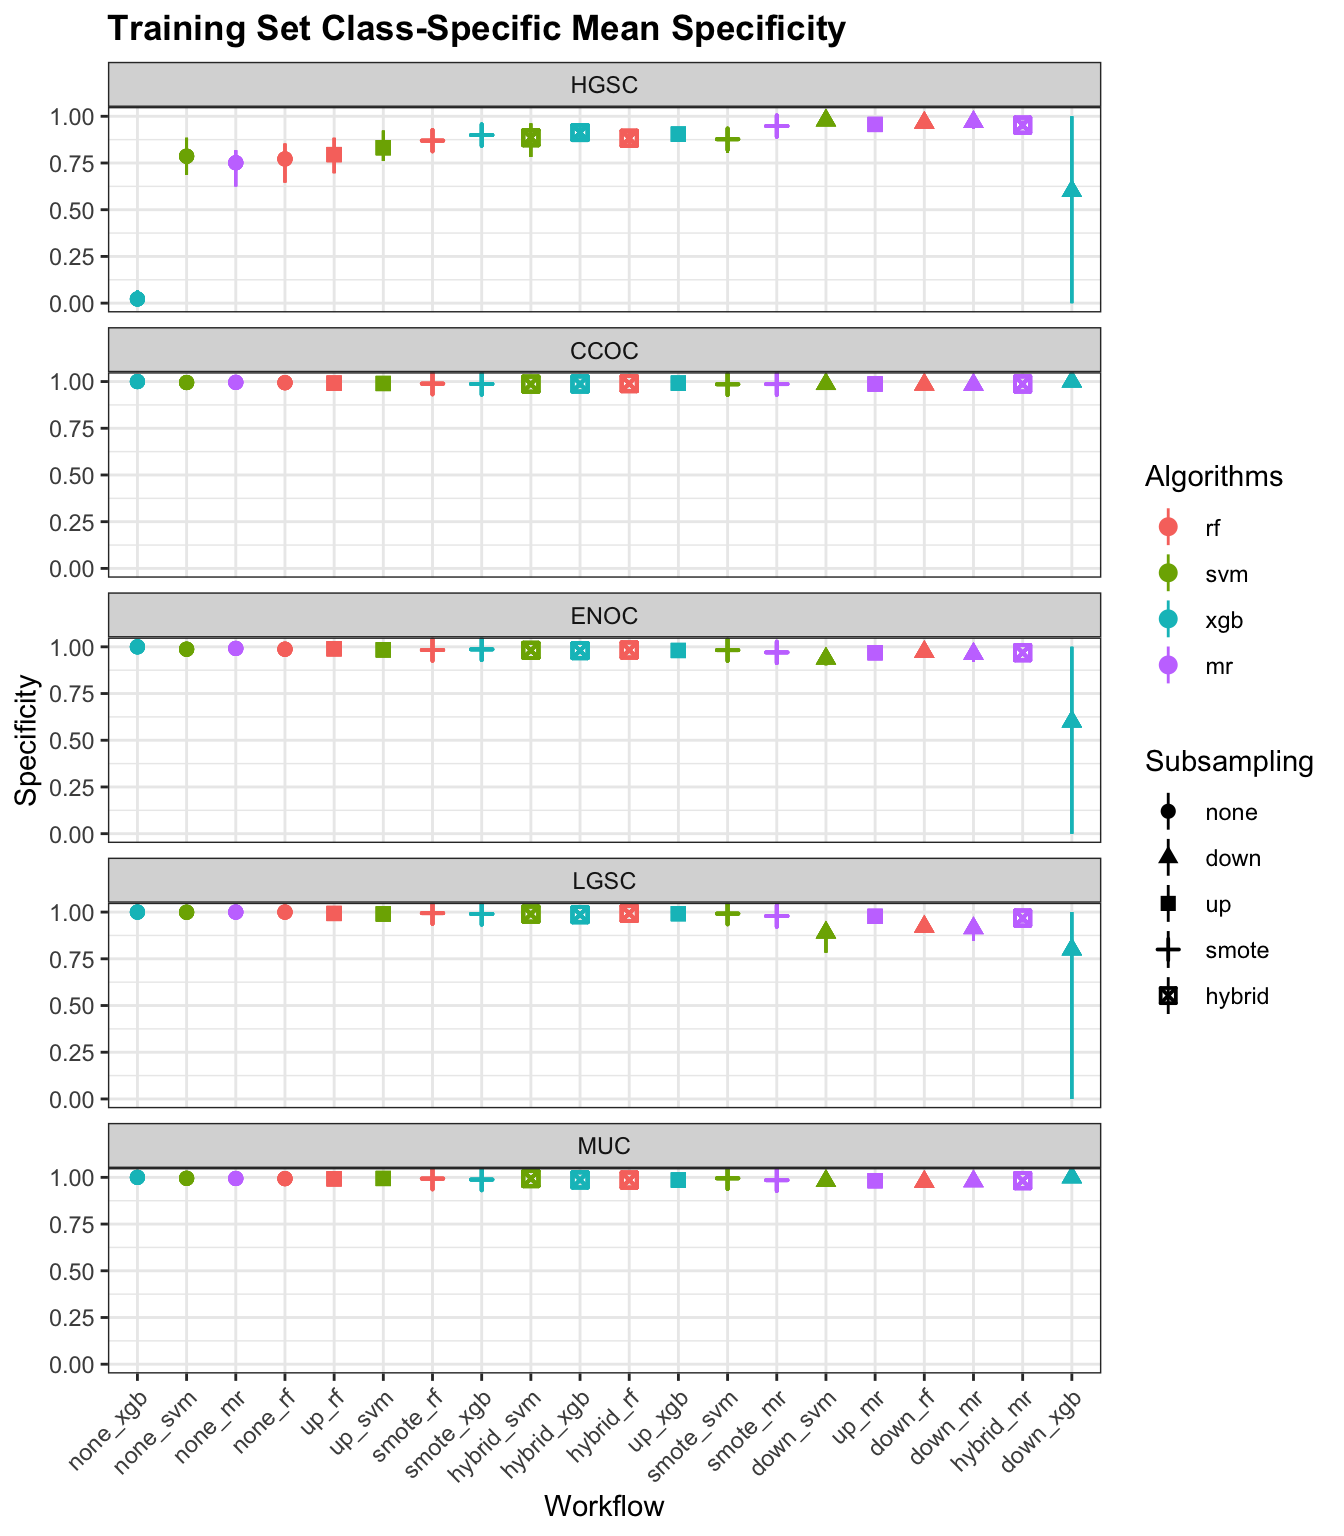
\includegraphics{OV_Histotypes_RSF_files/figure-latex/train-spec-class-1} 

}

\caption{Training Set Class-Specific Mean Specificity}\label{fig:train-spec-class}
\end{figure}

\begin{table}

\caption{\label{tab:train-spec-class-table}Cross-Validated Training Set Class-Specific Mean Specificity}
\centering
\begin{tabular}[t]{l|l|l|l|l|l}
\hline
\multicolumn{2}{c|}{ } & \multicolumn{4}{c}{Algorithms} \\
\cline{3-6}
Subsampling & Histotype & rf & svm & xgb & mr\\
\hline
 & HGSC & 0.682 & 0.776 & 0 & 0.005\\
\cline{2-6}
 & CCOC & 0.996 & 0.996 & \cellcolor[HTML]{90ee90}{1} & \cellcolor[HTML]{90ee90}{1}\\
\cline{2-6}
 & ENOC & 0.992 & 0.988 & \cellcolor[HTML]{90ee90}{1} & \cellcolor[HTML]{90ee90}{1}\\
\cline{2-6}
 & LGSC & \cellcolor[HTML]{90ee90}{1} & 0.999 & \cellcolor[HTML]{90ee90}{1} & \cellcolor[HTML]{90ee90}{1}\\
\cline{2-6}
\multirow{-5}{*}{\raggedright\arraybackslash none} & MUC & 0.993 & 0.995 & \cellcolor[HTML]{90ee90}{1} & \cellcolor[HTML]{90ee90}{1}\\
\cline{1-6}
 & HGSC & 0.962 & 0.97 & 0.8 & 0.966\\
\cline{2-6}
 & CCOC & 0.982 & 0.979 & \cellcolor[HTML]{90ee90}{1} & 0.985\\
\cline{2-6}
 & ENOC & 0.978 & 0.936 & \cellcolor[HTML]{90ee90}{1} & 0.958\\
\cline{2-6}
 & LGSC & 0.928 & 0.903 & 0.6 & 0.926\\
\cline{2-6}
\multirow{-5}{*}{\raggedright\arraybackslash down} & MUC & 0.967 & 0.987 & 0.6 & 0.979\\
\cline{1-6}
 & HGSC & 0.824 & 0.845 & 0.88 & 0.953\\
\cline{2-6}
 & CCOC & 0.995 & 0.99 & 0.994 & 0.988\\
\cline{2-6}
 & ENOC & 0.991 & 0.981 & 0.985 & 0.964\\
\cline{2-6}
 & LGSC & 0.996 & 0.992 & 0.994 & 0.964\\
\cline{2-6}
\multirow{-5}{*}{\raggedright\arraybackslash up} & MUC & 0.992 & 0.995 & 0.987 & 0.982\\
\cline{1-6}
 & HGSC & 0.854 & 0.803 & 0.901 & 0.939\\
\cline{2-6}
 & CCOC & 0.99 & 0.991 & 0.991 & 0.99\\
\cline{2-6}
 & ENOC & 0.986 & 0.983 & 0.983 & 0.97\\
\cline{2-6}
 & LGSC & 0.994 & 0.995 & 0.989 & 0.97\\
\cline{2-6}
\multirow{-5}{*}{\raggedright\arraybackslash smote} & MUC & 0.991 & 0.996 & 0.987 & 0.984\\
\cline{1-6}
 & HGSC & 0.901 & 0.892 & 0.896 & 0.944\\
\cline{2-6}
 & CCOC & 0.993 & 0.991 & 0.989 & 0.99\\
\cline{2-6}
 & ENOC & 0.983 & 0.975 & 0.981 & 0.969\\
\cline{2-6}
 & LGSC & 0.993 & 0.989 & 0.988 & 0.973\\
\cline{2-6}
\multirow{-5}{*}{\raggedright\arraybackslash hybrid} & MUC & 0.987 & 0.992 & 0.986 & 0.983\\
\hline
\end{tabular}
\end{table}

\subsection{F1-Score}\label{f1-score-1}

\begin{figure}[H]

{\centering 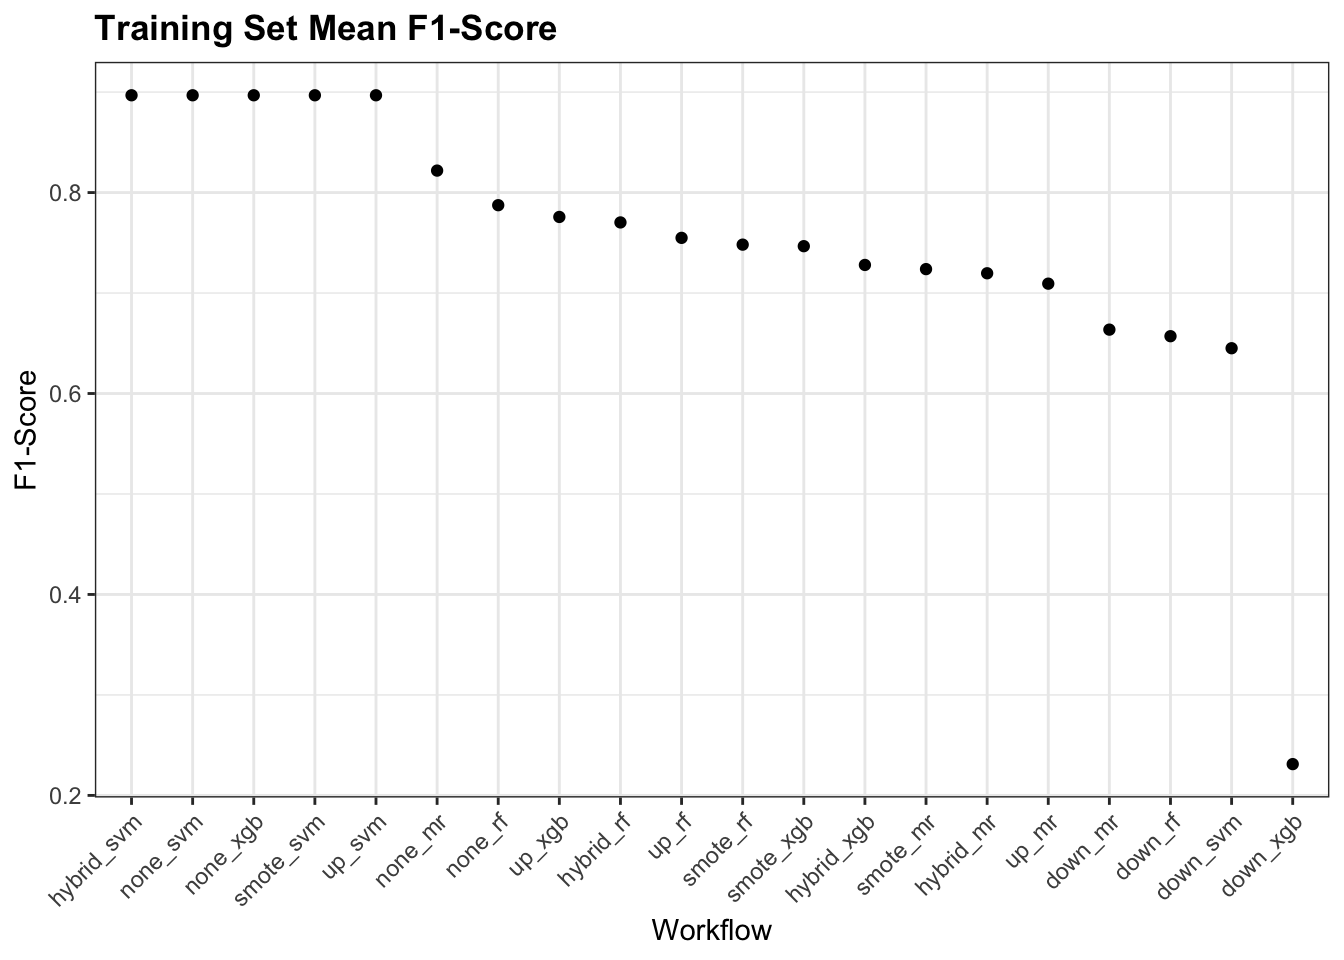
\includegraphics{OV_Histotypes_RSF_files/figure-latex/train-f1-1} 

}

\caption{Training Set Mean F1-Score}\label{fig:train-f1}
\end{figure}

\begin{table}

\caption{\label{tab:train-f1-table}Training Set Mean F1-Score}
\centering
\begin{tabular}[t]{l|l|l|l|l}
\hline
\multicolumn{1}{c|}{ } & \multicolumn{4}{c}{Algorithms} \\
\cline{2-5}
Subsampling & rf & svm & xgb & mr\\
\hline
none & \cellcolor[HTML]{FF0000}{0.787} & \cellcolor[HTML]{FFD700}{0.801} & \cellcolor[HTML]{FF0000}{0.897} & \cellcolor[HTML]{FF0000}{0.822}\\
\hline
down & 0.657 & 0.645 & \cellcolor[HTML]{FF0000}{0.231} & 0.664\\
\hline
up & \cellcolor[HTML]{FFD700}{0.755} & 0.726 & \cellcolor[HTML]{FFD700}{0.776} & 0.709\\
\hline
smote & \cellcolor[HTML]{FFD700}{0.748} & \cellcolor[HTML]{FFD700}{0.75} & 0.747 & 0.724\\
\hline
hybrid & \cellcolor[HTML]{90ee90}{0.77} & 0.751 & 0.728 & 0.72\\
\hline
\end{tabular}
\end{table}

\begin{figure}[H]

{\centering 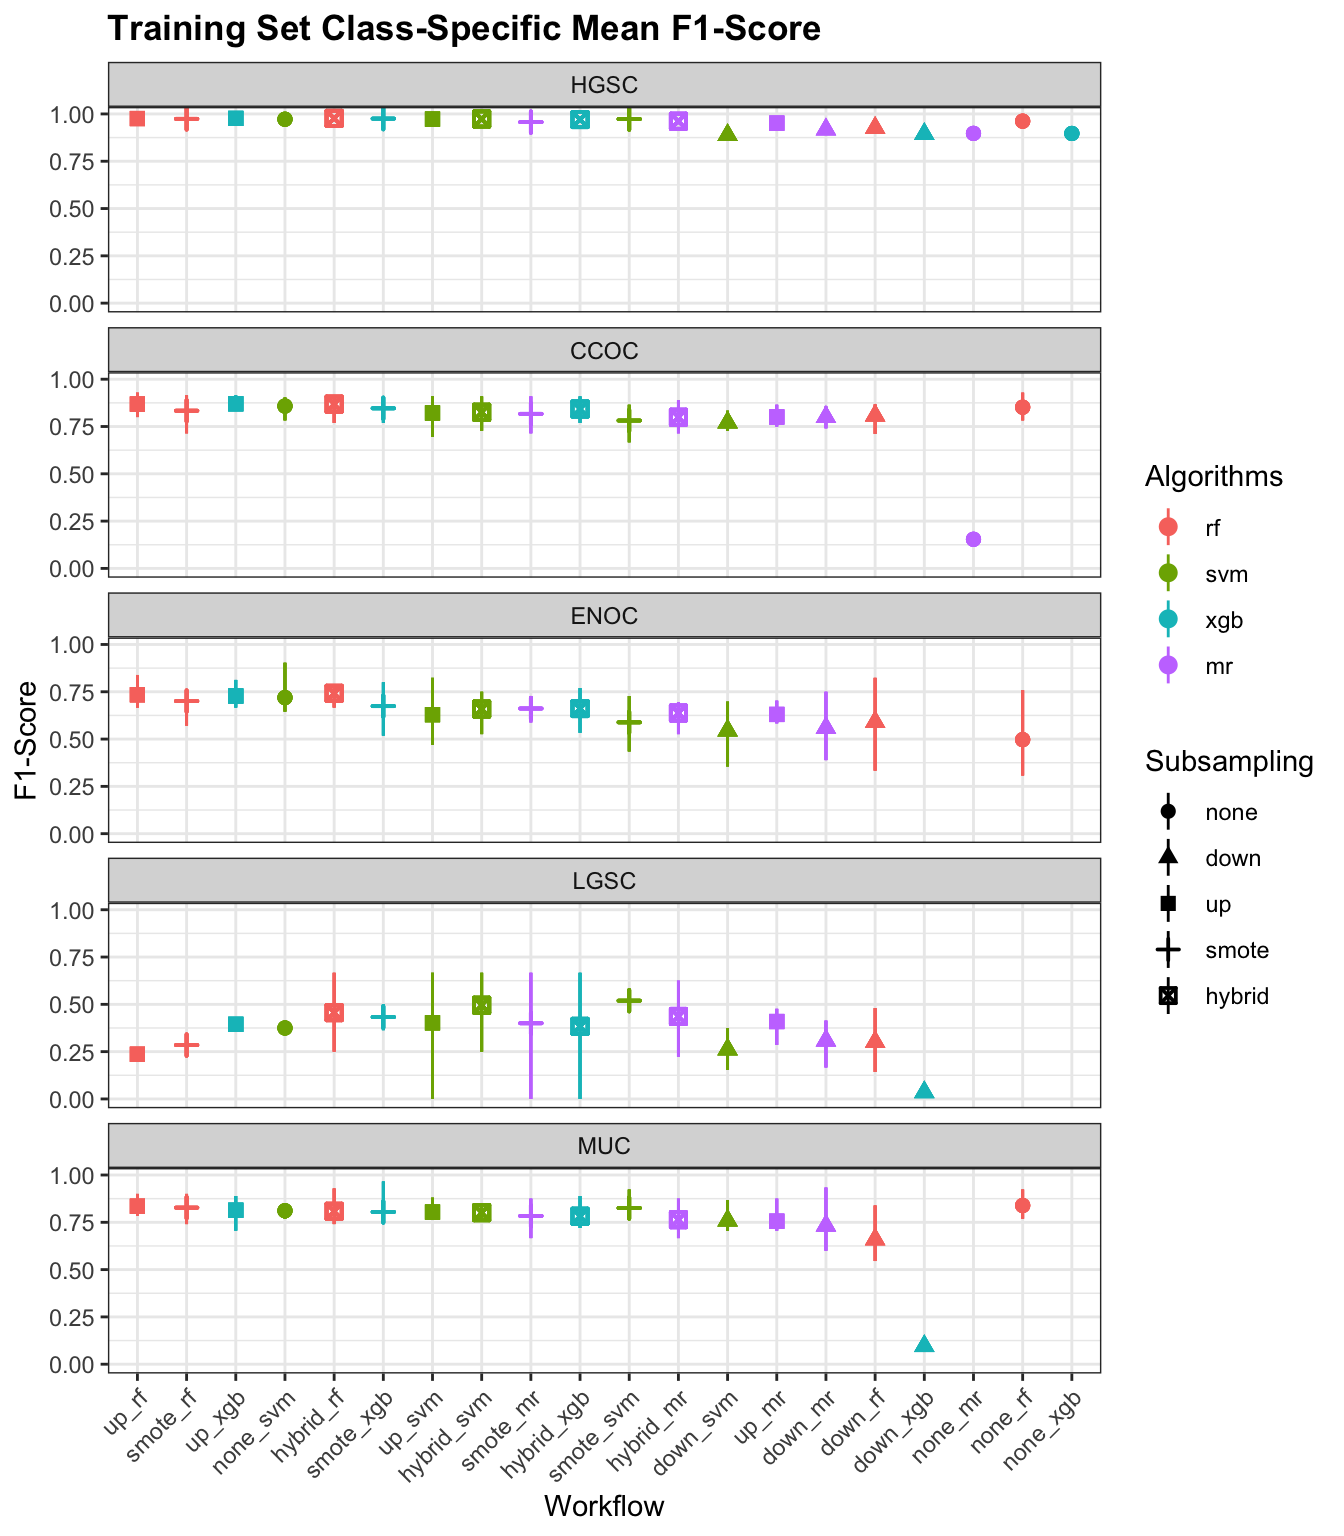
\includegraphics{OV_Histotypes_RSF_files/figure-latex/train-f1-class-1} 

}

\caption{Training Set Class-Specific Mean F1-Score}\label{fig:train-f1-class}
\end{figure}

\begin{table}

\caption{\label{tab:train-f1-class-table}Cross-Validated Training Set Class-Specific Mean F1-Score}
\centering
\begin{tabular}[t]{l|l|l|l|l|l}
\hline
\multicolumn{2}{c|}{ } & \multicolumn{4}{c}{Algorithms} \\
\cline{3-6}
Subsampling & Histotype & rf & svm & xgb & mr\\
\hline
 & HGSC & \cellcolor[HTML]{FF0000}{0.962} & \cellcolor[HTML]{FFD700}{0.972} & \cellcolor[HTML]{FF0000}{0.897} & \cellcolor[HTML]{FF0000}{0.897}\\
\cline{2-6}
 & CCOC & \cellcolor[HTML]{FF0000}{0.852} & \cellcolor[HTML]{FFD700}{0.858} & \cellcolor[HTML]{FF0000}{NaN} & \cellcolor[HTML]{FF0000}{0.154}\\
\cline{2-6}
 & ENOC & \cellcolor[HTML]{FF0000}{0.497} & \cellcolor[HTML]{FFD700}{0.719} & \cellcolor[HTML]{FF0000}{NaN} & \cellcolor[HTML]{FF0000}{NaN}\\
\cline{2-6}
 & LGSC & \cellcolor[HTML]{FF0000}{NaN} & \cellcolor[HTML]{FFD700}{0.375} & \cellcolor[HTML]{FF0000}{NaN} & \cellcolor[HTML]{FF0000}{NaN}\\
\cline{2-6}
\multirow{-5}{*}{\raggedright\arraybackslash none} & MUC & \cellcolor[HTML]{FF0000}{0.839} & \cellcolor[HTML]{FFD700}{0.811} & \cellcolor[HTML]{FF0000}{NaN} & \cellcolor[HTML]{FF0000}{NaN}\\
\cline{1-6}
 & HGSC & 0.926 & 0.888 & \cellcolor[HTML]{FF0000}{0.894} & 0.918\\
\cline{2-6}
 & CCOC & 0.808 & 0.771 & \cellcolor[HTML]{FF0000}{NaN} & 0.8\\
\cline{2-6}
 & ENOC & 0.59 & 0.545 & \cellcolor[HTML]{FF0000}{NaN} & 0.559\\
\cline{2-6}
 & LGSC & 0.301 & 0.262 & \cellcolor[HTML]{FF0000}{0.035} & 0.308\\
\cline{2-6}
\multirow{-5}{*}{\raggedright\arraybackslash down} & MUC & 0.66 & 0.759 & \cellcolor[HTML]{FF0000}{0.096} & 0.732\\
\cline{1-6}
 & HGSC & \cellcolor[HTML]{FFD700}{0.976} & 0.973 & \cellcolor[HTML]{FFD700}{0.976} & 0.951\\
\cline{2-6}
 & CCOC & \cellcolor[HTML]{FFD700}{0.869} & 0.822 & \cellcolor[HTML]{FFD700}{0.87} & 0.8\\
\cline{2-6}
 & ENOC & \cellcolor[HTML]{FFD700}{0.734} & 0.629 & \cellcolor[HTML]{FFD700}{0.728} & 0.63\\
\cline{2-6}
 & LGSC & \cellcolor[HTML]{FFD700}{0.236} & 0.402 & \cellcolor[HTML]{FFD700}{0.394} & 0.409\\
\cline{2-6}
\multirow{-5}{*}{\raggedright\arraybackslash up} & MUC & \cellcolor[HTML]{FFD700}{0.835} & 0.804 & \cellcolor[HTML]{FFD700}{0.814} & 0.756\\
\cline{1-6}
 & HGSC & \cellcolor[HTML]{FFD700}{0.974} & \cellcolor[HTML]{FFD700}{0.973} & 0.975 & 0.957\\
\cline{2-6}
 & CCOC & \cellcolor[HTML]{FFD700}{0.833} & \cellcolor[HTML]{FFD700}{0.782} & 0.846 & 0.817\\
\cline{2-6}
 & ENOC & \cellcolor[HTML]{FFD700}{0.701} & \cellcolor[HTML]{FFD700}{0.588} & 0.674 & 0.662\\
\cline{2-6}
 & LGSC & \cellcolor[HTML]{FFD700}{0.285} & \cellcolor[HTML]{FFD700}{0.519} & 0.433 & 0.4\\
\cline{2-6}
\multirow{-5}{*}{\raggedright\arraybackslash smote} & MUC & \cellcolor[HTML]{FFD700}{0.827} & \cellcolor[HTML]{FFD700}{0.825} & 0.805 & 0.784\\
\cline{1-6}
 & HGSC & \cellcolor[HTML]{90ee90}{0.977} & 0.973 & 0.97 & 0.962\\
\cline{2-6}
 & CCOC & 0.868 & 0.825 & 0.843 & 0.799\\
\cline{2-6}
 & ENOC & 0.742 & 0.659 & 0.661 & 0.638\\
\cline{2-6}
 & LGSC & 0.456 & 0.495 & 0.384 & 0.436\\
\cline{2-6}
\multirow{-5}{*}{\raggedright\arraybackslash hybrid} & MUC & 0.808 & 0.801 & 0.782 & 0.764\\
\hline
\end{tabular}
\end{table}

\subsection{Balanced Accuracy}\label{balanced-accuracy-1}

\begin{figure}[H]

{\centering 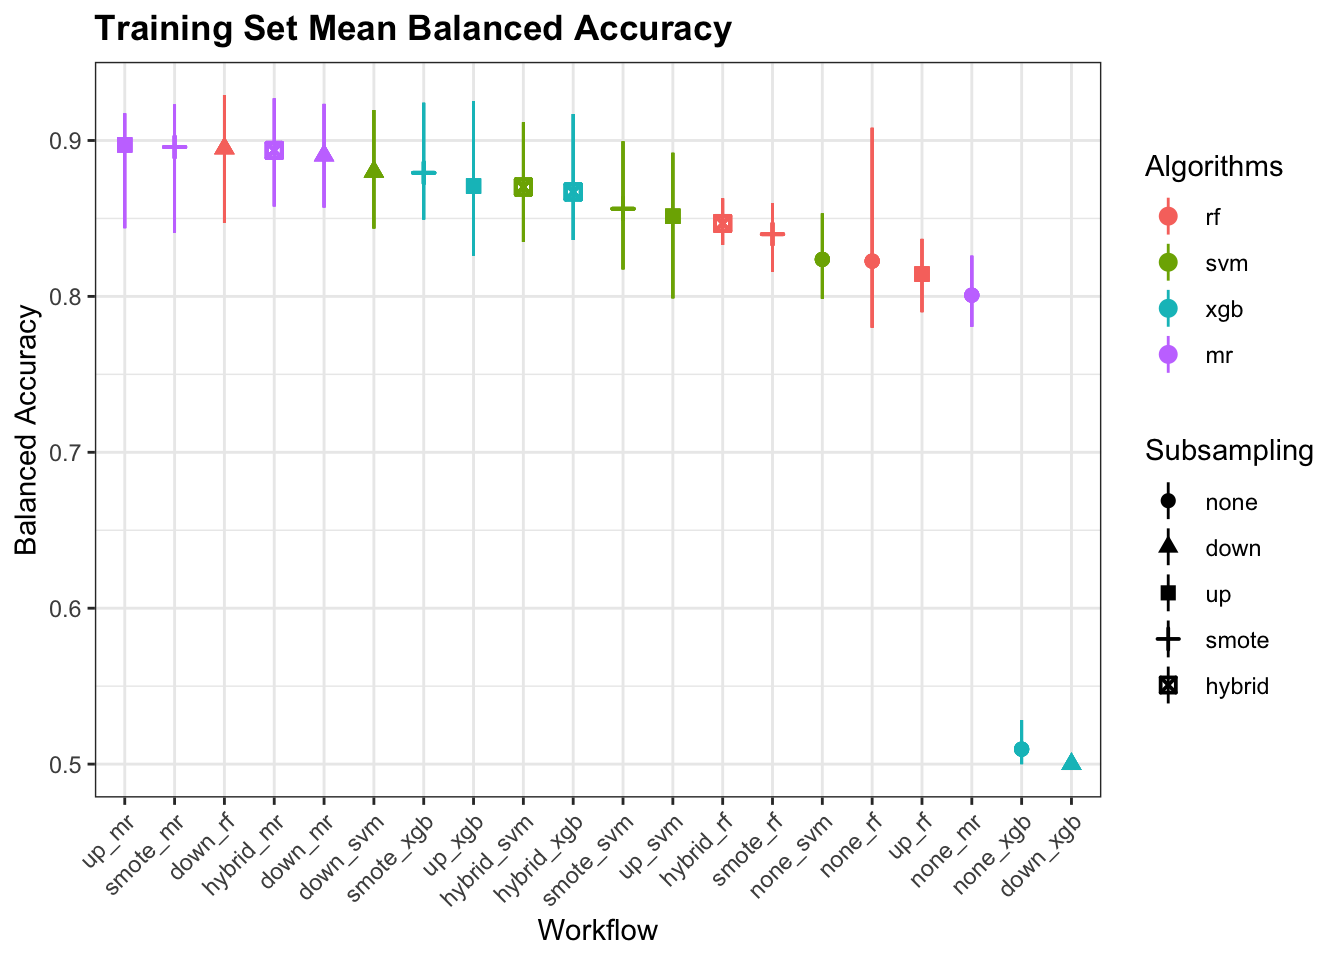
\includegraphics{OV_Histotypes_RSF_files/figure-latex/train-bal-accuracy-1} 

}

\caption{Training Set Mean Balanced Accuracy}\label{fig:train-bal-accuracy}
\end{figure}

\begin{table}

\caption{\label{tab:train-bal-accuracy-table}Training Set Mean Balanced Accuracy}
\centering
\begin{tabular}[t]{l|l|l|l|l}
\hline
\multicolumn{1}{c|}{ } & \multicolumn{4}{c}{Algorithms} \\
\cline{2-5}
Subsampling & rf & svm & xgb & mr\\
\hline
none & 0.767 & 0.81 & 0.5 & 0.502\\
\hline
down & 0.884 & \cellcolor[HTML]{90ee90}{0.897} & 0.5 & 0.896\\
\hline
up & 0.828 & 0.837 & 0.852 & 0.895\\
\hline
smote & 0.835 & 0.818 & 0.867 & 0.886\\
\hline
hybrid & 0.871 & 0.863 & 0.861 & 0.884\\
\hline
\end{tabular}
\end{table}

\begin{figure}[H]

{\centering 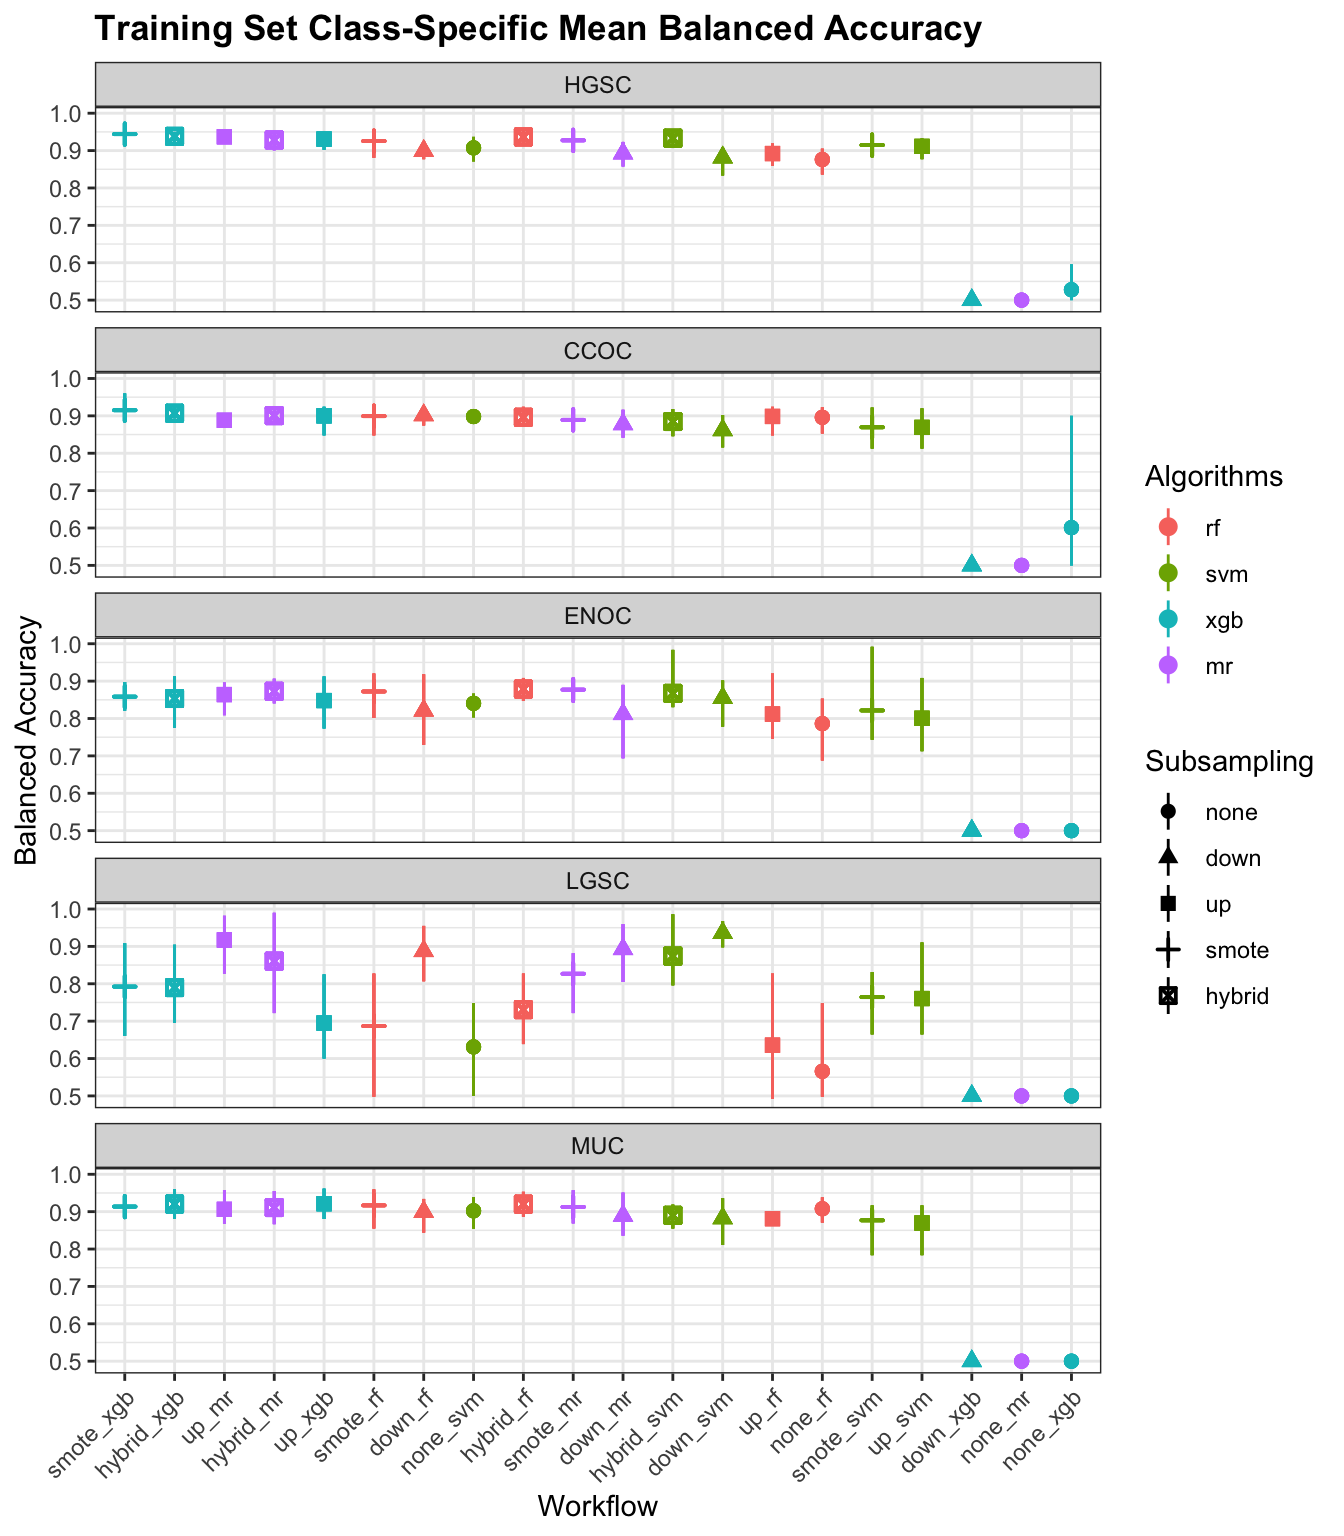
\includegraphics{OV_Histotypes_RSF_files/figure-latex/train-bal-accuracy-class-1} 

}

\caption{Training Set Class-Specific Mean Balanced Accuracy}\label{fig:train-bal-accuracy-class}
\end{figure}

\begin{table}

\caption{\label{tab:train-bal-accuracy-class-table}Training Set Class-Specific Mean Balanced Accuracy}
\centering
\begin{tabular}[t]{l|l|l|l|l|l}
\hline
\multicolumn{2}{c|}{ } & \multicolumn{4}{c}{Algorithms} \\
\cline{3-6}
Subsampling & Histotype & rf & svm & xgb & mr\\
\hline
 & HGSC & 0.838 & 0.885 & 0.5 & 0.502\\
\cline{2-6}
 & CCOC & 0.894 & 0.899 & 0.5 & 0.508\\
\cline{2-6}
 & ENOC & 0.696 & 0.836 & 0.5 & 0.5\\
\cline{2-6}
 & LGSC & 0.5 & 0.55 & 0.5 & 0.5\\
\cline{2-6}
\multirow{-5}{*}{\raggedright\arraybackslash none} & MUC & 0.908 & 0.879 & 0.5 & 0.5\\
\cline{1-6}
 & HGSC & 0.916 & 0.887 & 0.5 & 0.911\\
\cline{2-6}
 & CCOC & 0.914 & 0.902 & 0.5 & 0.901\\
\cline{2-6}
 & ENOC & 0.792 & 0.862 & 0.5 & 0.822\\
\cline{2-6}
 & LGSC & 0.897 & 0.935 & 0.5 & 0.929\\
\cline{2-6}
\multirow{-5}{*}{\raggedright\arraybackslash down} & MUC & 0.902 & 0.896 & 0.5 & 0.915\\
\cline{1-6}
 & HGSC & 0.908 & 0.913 & 0.93 & 0.935\\
\cline{2-6}
 & CCOC & 0.913 & 0.899 & 0.917 & 0.887\\
\cline{2-6}
 & ENOC & 0.837 & 0.805 & 0.855 & 0.857\\
\cline{2-6}
 & LGSC & 0.565 & 0.696 & 0.63 & 0.882\\
\cline{2-6}
\multirow{-5}{*}{\raggedright\arraybackslash up} & MUC & 0.92 & 0.873 & 0.93 & 0.914\\
\cline{1-6}
 & HGSC & 0.918 & 0.897 & 0.937 & 0.935\\
\cline{2-6}
 & CCOC & 0.91 & 0.86 & 0.915 & 0.894\\
\cline{2-6}
 & ENOC & 0.832 & 0.773 & 0.826 & 0.855\\
\cline{2-6}
 & LGSC & 0.597 & 0.681 & 0.728 & 0.818\\
\cline{2-6}
\multirow{-5}{*}{\raggedright\arraybackslash smote} & MUC & 0.92 & 0.881 & 0.931 & 0.93\\
\cline{1-6}
 & HGSC & 0.939 & 0.931 & 0.93 & \cellcolor[HTML]{90ee90}{0.941}\\
\cline{2-6}
 & CCOC & 0.922 & 0.893 & 0.92 & 0.88\\
\cline{2-6}
 & ENOC & 0.874 & 0.848 & 0.827 & 0.848\\
\cline{2-6}
 & LGSC & 0.697 & 0.761 & 0.711 & 0.837\\
\cline{2-6}
\multirow{-5}{*}{\raggedright\arraybackslash hybrid} & MUC & 0.925 & 0.881 & 0.917 & 0.914\\
\hline
\end{tabular}
\end{table}

\subsection{Kappa}\label{kappa-1}

\begin{figure}[H]

{\centering 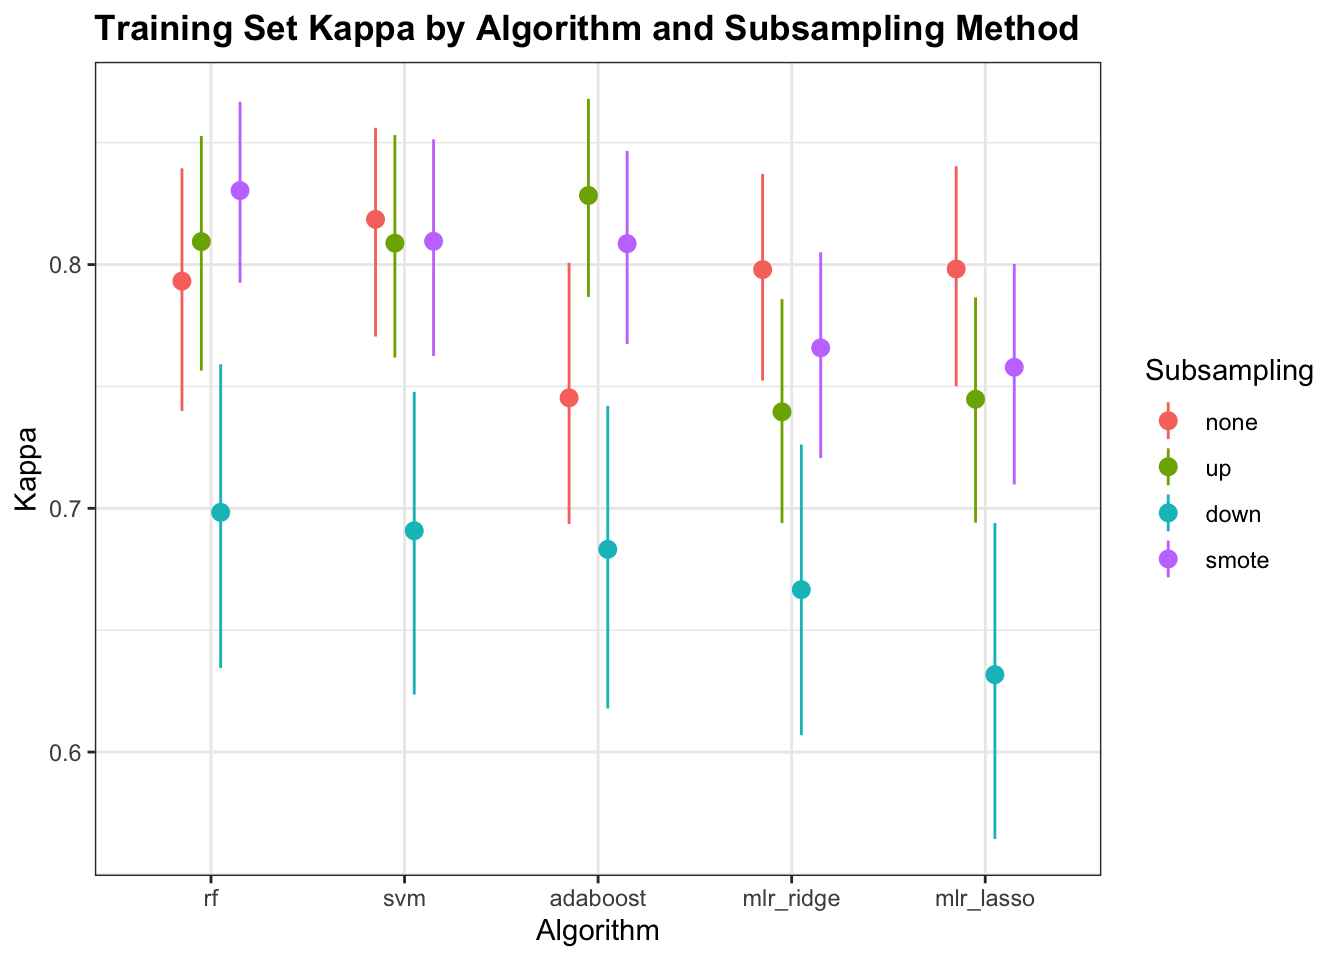
\includegraphics{OV_Histotypes_RSF_files/figure-latex/train-kappa-1} 

}

\caption{Training Set Mean Kappa}\label{fig:train-kappa}
\end{figure}

\begin{table}

\caption{\label{tab:train-kappa-table}Training Set Mean Kappa}
\centering
\begin{tabular}[t]{l|l|l|l|l}
\hline
\multicolumn{1}{c|}{ } & \multicolumn{4}{c}{Algorithms} \\
\cline{2-5}
Subsampling & rf & svm & xgb & mr\\
\hline
none & 0.727 & 0.79 & 0 & 0.008\\
\hline
down & 0.639 & 0.569 & 0 & 0.63\\
\hline
up & 0.81 & 0.783 & 0.814 & 0.717\\
\hline
smote & 0.796 & 0.772 & 0.799 & 0.743\\
\hline
hybrid & \cellcolor[HTML]{90ee90}{0.819} & 0.788 & 0.783 & 0.744\\
\hline
\end{tabular}
\end{table}

\begin{figure}[H]

{\centering 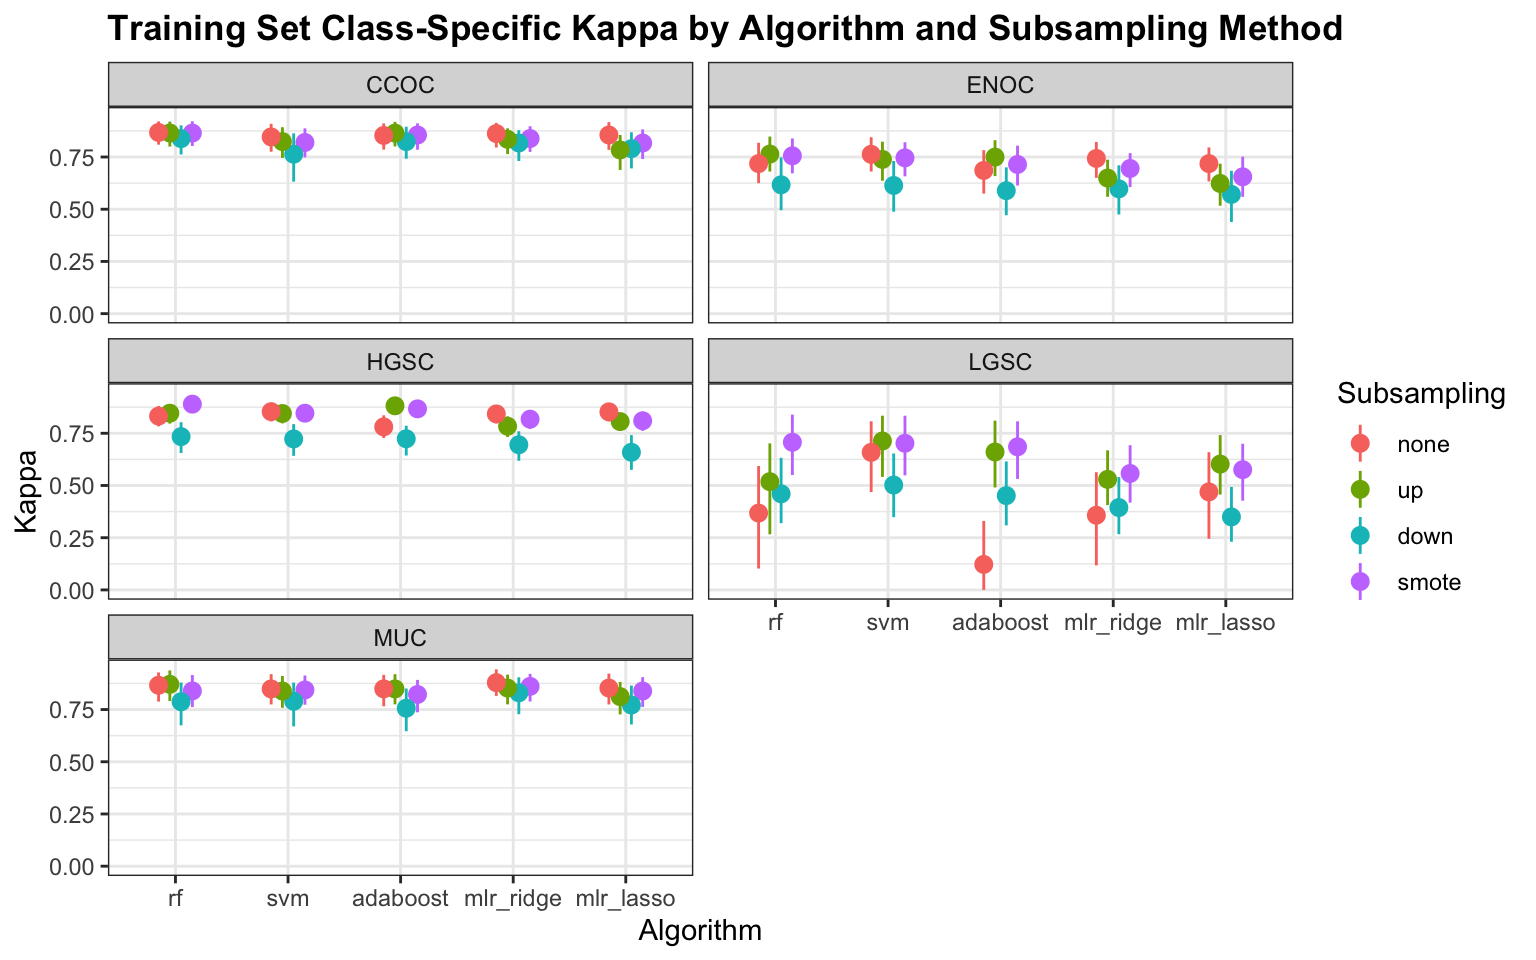
\includegraphics{OV_Histotypes_RSF_files/figure-latex/train-kappa-class-1} 

}

\caption{Training Set Class-Specific Mean Kappa}\label{fig:train-kappa-class}
\end{figure}

\begin{table}

\caption{\label{tab:train-kappa-class-table}Training Set Class-Specific Mean Kappa}
\centering
\begin{tabular}[t]{l|l|l|l|l|l}
\hline
\multicolumn{2}{c|}{ } & \multicolumn{4}{c}{Algorithms} \\
\cline{3-6}
Subsampling & Histotype & rf & svm & xgb & mr\\
\hline
 & HGSC & 0.761 & 0.834 & 0 & 0.008\\
\cline{2-6}
 & CCOC & 0.843 & 0.849 & 0 & 0.03\\
\cline{2-6}
 & ENOC & 0.479 & 0.705 & 0 & 0\\
\cline{2-6}
 & LGSC & 0 & 0.148 & 0 & 0\\
\cline{2-6}
\multirow{-5}{*}{\raggedright\arraybackslash none} & MUC & 0.83 & 0.803 & 0 & 0\\
\cline{1-6}
 & HGSC & 0.695 & 0.589 & 0 & 0.671\\
\cline{2-6}
 & CCOC & 0.793 & 0.755 & 0 & 0.786\\
\cline{2-6}
 & ENOC & 0.57 & 0.512 & 0 & 0.531\\
\cline{2-6}
 & LGSC & 0.281 & 0.238 & 0 & 0.288\\
\cline{2-6}
\multirow{-5}{*}{\raggedright\arraybackslash down} & MUC & 0.64 & 0.747 & 0 & 0.718\\
\cline{1-6}
 & HGSC & 0.86 & 0.848 & 0.872 & 0.776\\
\cline{2-6}
 & CCOC & 0.86 & 0.81 & 0.861 & 0.787\\
\cline{2-6}
 & ENOC & 0.721 & 0.61 & 0.713 & 0.607\\
\cline{2-6}
 & LGSC & 0.181 & 0.394 & 0.307 & 0.394\\
\cline{2-6}
\multirow{-5}{*}{\raggedright\arraybackslash up} & MUC & 0.826 & 0.795 & 0.804 & 0.743\\
\cline{1-6}
 & HGSC & 0.856 & 0.842 & 0.869 & 0.795\\
\cline{2-6}
 & CCOC & 0.822 & 0.769 & 0.836 & 0.805\\
\cline{2-6}
 & ENOC & 0.685 & 0.569 & 0.657 & 0.64\\
\cline{2-6}
 & LGSC & 0.22 & 0.409 & 0.422 & 0.386\\
\cline{2-6}
\multirow{-5}{*}{\raggedright\arraybackslash smote} & MUC & 0.818 & 0.817 & 0.795 & 0.772\\
\cline{1-6}
 & HGSC & \cellcolor[HTML]{90ee90}{0.876} & 0.857 & 0.844 & 0.815\\
\cline{2-6}
 & CCOC & 0.86 & 0.814 & 0.832 & 0.786\\
\cline{2-6}
 & ENOC & 0.728 & 0.639 & 0.644 & 0.615\\
\cline{2-6}
 & LGSC & 0.448 & 0.486 & 0.373 & 0.423\\
\cline{2-6}
\multirow{-5}{*}{\raggedright\arraybackslash hybrid} & MUC & 0.798 & 0.791 & 0.771 & 0.751\\
\hline
\end{tabular}
\end{table}

\subsection{G-mean}\label{g-mean}

\begin{figure}[H]

{\centering 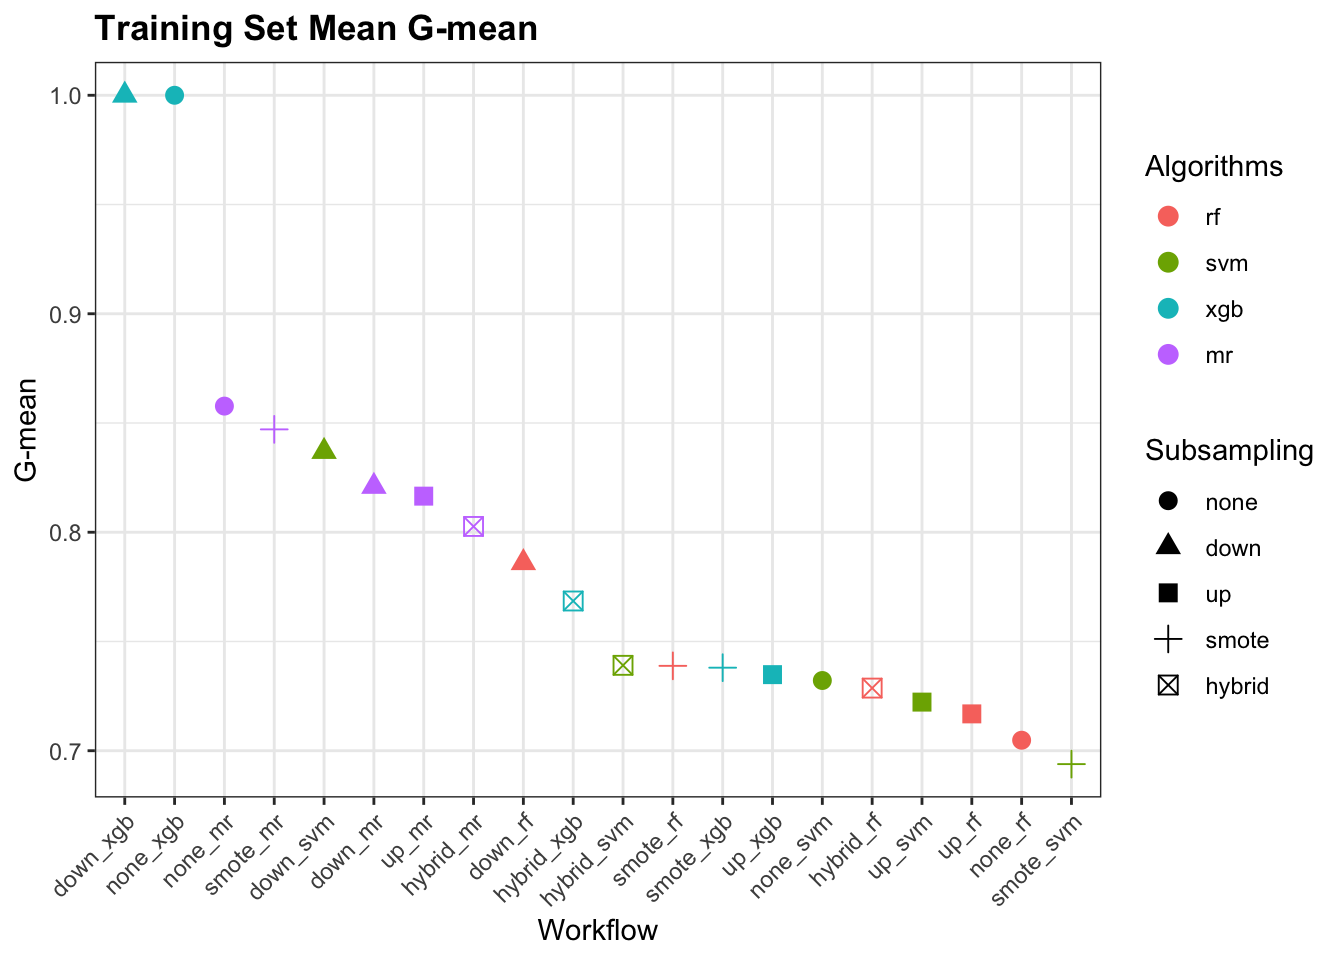
\includegraphics{OV_Histotypes_RSF_files/figure-latex/train-gmean-1} 

}

\caption{Training Set Mean G-mean}\label{fig:train-gmean}
\end{figure}

\begin{table}

\caption{\label{tab:train-gmean-table}Training Set Mean G-mean}
\centering
\begin{tabular}[t]{l|l|l|l|l}
\hline
\multicolumn{1}{c|}{ } & \multicolumn{4}{c}{Algorithms} \\
\cline{2-5}
Subsampling & rf & svm & xgb & mr\\
\hline
none & 0 & 0.255 & 0 & 0\\
\hline
down & 0.784 & \cellcolor[HTML]{90ee90}{0.831} & 0 & 0.815\\
\hline
up & 0.375 & 0.561 & 0.555 & 0.809\\
\hline
smote & 0.393 & 0.524 & 0.732 & 0.653\\
\hline
hybrid & 0.725 & 0.732 & 0.597 & 0.784\\
\hline
\end{tabular}
\end{table}

\begin{figure}[H]

{\centering 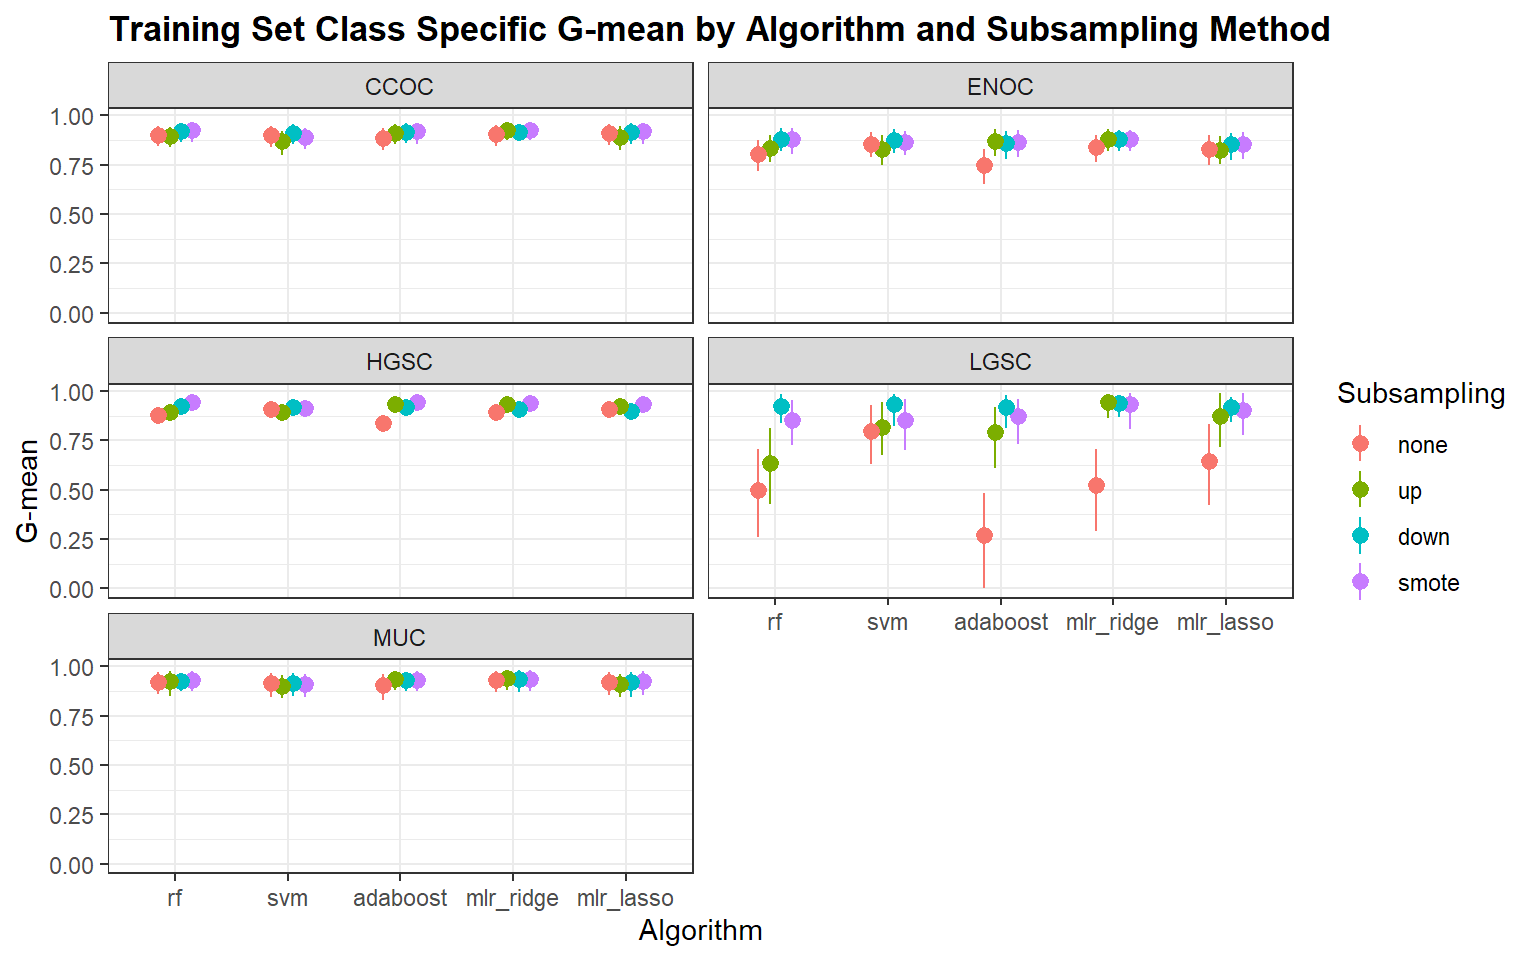
\includegraphics{OV_Histotypes_RSF_files/figure-latex/train-gmean-class-1} 

}

\caption{Training Set Class-Specific Mean G-mean}\label{fig:train-gmean-class}
\end{figure}

\begin{table}

\caption{\label{tab:train-gmean-class-table}Training Set Class-Specific Mean G-mean}
\centering
\begin{tabular}[t]{l|l|l|l|l|l}
\hline
\multicolumn{2}{c|}{ } & \multicolumn{4}{c}{Algorithms} \\
\cline{3-6}
Subsampling & Histotype & rf & svm & xgb & mr\\
\hline
 & HGSC & 0.823 & 0.878 & 0 & 0.03\\
\cline{2-6}
 & CCOC & 0.888 & 0.893 & 0 & 0.058\\
\cline{2-6}
 & ENOC & 0.615 & 0.818 & 0 & 0\\
\cline{2-6}
 & LGSC & 0 & 0.197 & 0 & 0\\
\cline{2-6}
\multirow{-5}{*}{\raggedright\arraybackslash none} & MUC & 0.901 & 0.87 & 0 & 0\\
\cline{1-6}
 & HGSC & 0.915 & 0.883 & 0 & 0.909\\
\cline{2-6}
 & CCOC & 0.911 & 0.898 & 0 & 0.897\\
\cline{2-6}
 & ENOC & 0.758 & 0.857 & 0 & 0.803\\
\cline{2-6}
 & LGSC & 0.892 & 0.934 & 0 & 0.926\\
\cline{2-6}
\multirow{-5}{*}{\raggedright\arraybackslash down} & MUC & 0.897 & 0.888 & 0 & 0.909\\
\cline{1-6}
 & HGSC & 0.904 & 0.91 & 0.928 & 0.935\\
\cline{2-6}
 & CCOC & 0.908 & 0.893 & 0.913 & 0.881\\
\cline{2-6}
 & ENOC & 0.82 & 0.779 & 0.843 & 0.844\\
\cline{2-6}
 & LGSC & 0.278 & 0.555 & 0.453 & 0.876\\
\cline{2-6}
\multirow{-5}{*}{\raggedright\arraybackslash up} & MUC & 0.915 & 0.862 & 0.927 & 0.906\\
\cline{1-6}
 & HGSC & 0.915 & 0.891 & 0.937 & 0.934\\
\cline{2-6}
 & CCOC & 0.906 & 0.847 & 0.912 & 0.887\\
\cline{2-6}
 & ENOC & 0.814 & 0.735 & 0.805 & 0.844\\
\cline{2-6}
 & LGSC & 0.325 & 0.534 & 0.673 & 0.717\\
\cline{2-6}
\multirow{-5}{*}{\raggedright\arraybackslash smote} & MUC & 0.914 & 0.87 & 0.926 & 0.925\\
\cline{1-6}
 & HGSC & 0.938 & 0.93 & 0.929 & \cellcolor[HTML]{90ee90}{0.941}\\
\cline{2-6}
 & CCOC & 0.919 & 0.886 & 0.917 & 0.871\\
\cline{2-6}
 & ENOC & 0.864 & 0.834 & 0.802 & 0.837\\
\cline{2-6}
 & LGSC & 0.615 & 0.714 & 0.579 & 0.822\\
\cline{2-6}
\multirow{-5}{*}{\raggedright\arraybackslash hybrid} & MUC & 0.919 & 0.872 & 0.911 & 0.908\\
\hline
\end{tabular}
\end{table}

\section{Rank Aggregation}\label{rank-aggregation}

\begin{center}\includegraphics{OV_Histotypes_RSF_files/figure-latex/per-class-metrics-1} \end{center}

The 18 workflows are ordered in the table by their aggregated ranks using the Genetic Algorithm. We see that the best performing methods involve the sequential and two-step algorithms.

\subsection{Top Workflows}\label{top-workflows}

We look at the per-class evaluation metrics of the top 4 workflows.

\begin{figure}[H]

{\centering 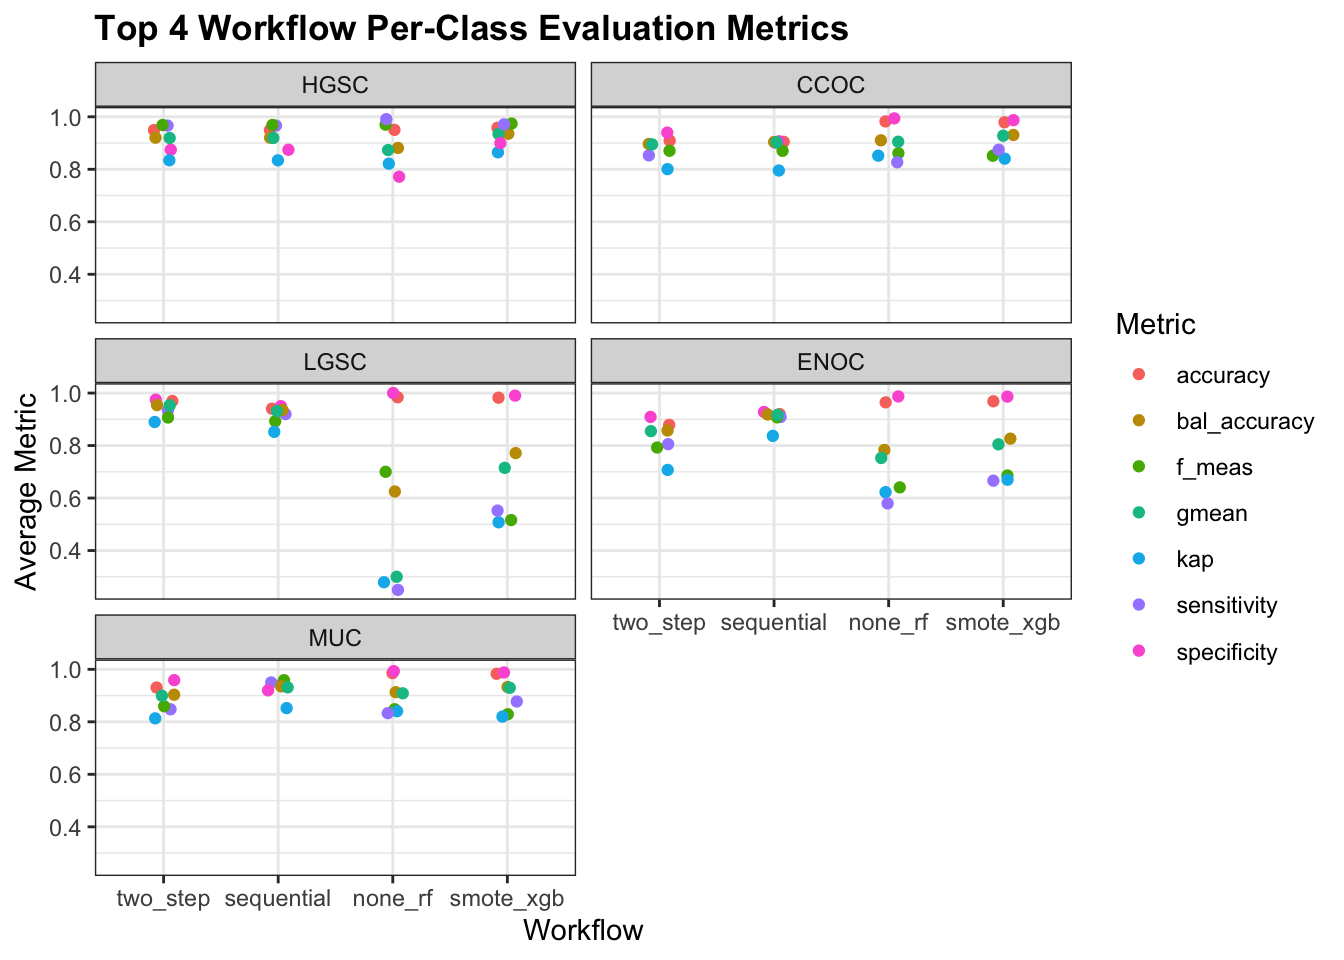
\includegraphics{OV_Histotypes_RSF_files/figure-latex/metrics-top4-1} 

}

\caption{Top 4 Workflow Per-Class Evaluation Metrics}\label{fig:metrics-top4}
\end{figure}

\begin{figure}[H]

{\centering 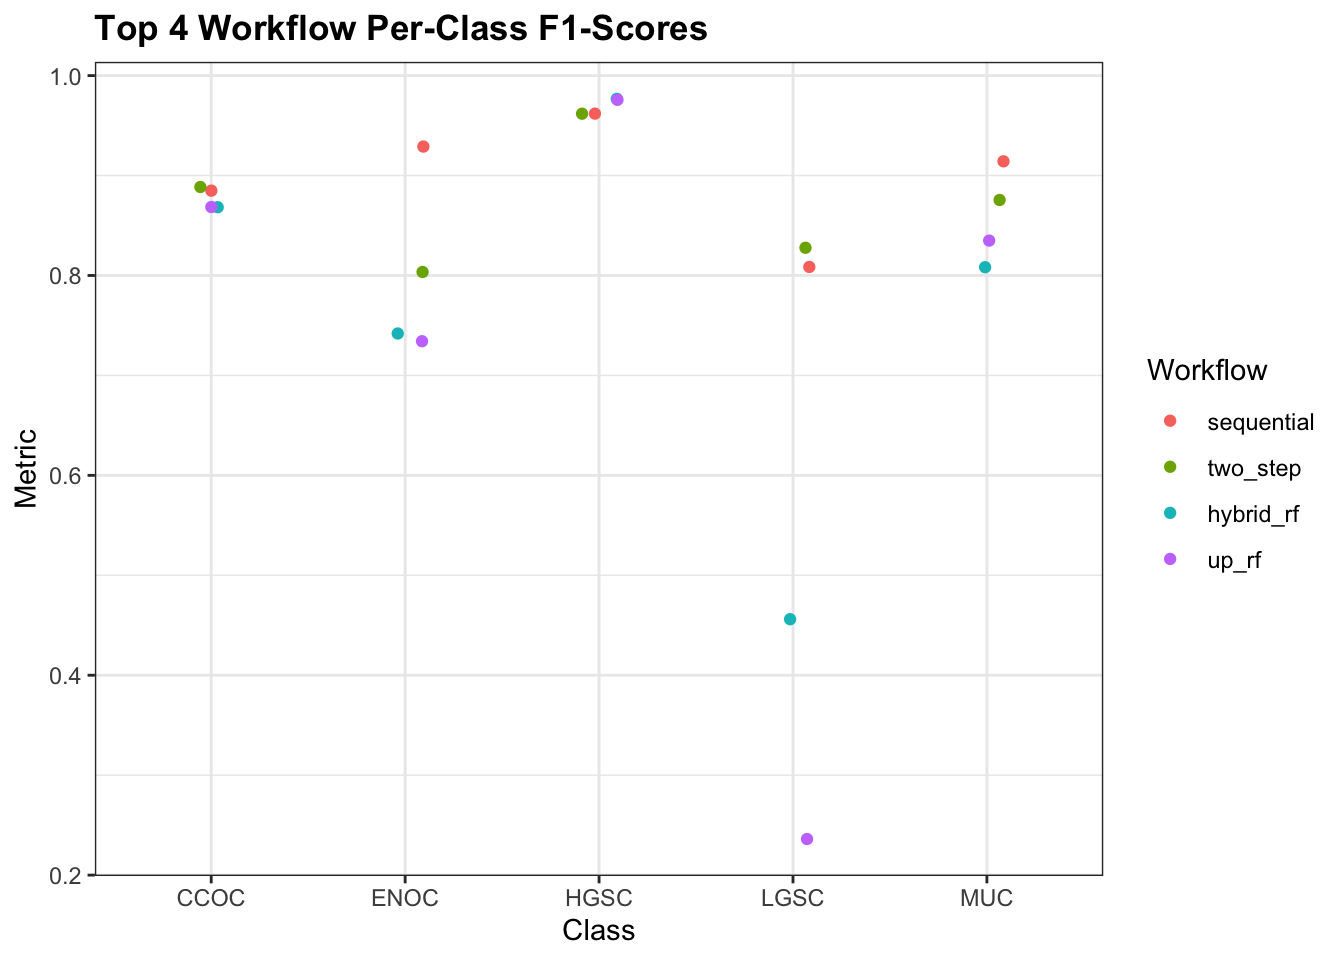
\includegraphics{OV_Histotypes_RSF_files/figure-latex/metrics-f1-top4-1} 

}

\caption{Top 4 Workflow Per-Class F1-Scores}\label{fig:metrics-f1-top4}
\end{figure}

Misclassified cases from a previous step of the sequence of classifiers are not included in subsequent steps of the training set CV folds. Thus, we cannot piece together the test set predictions from the sequential and two-step algorithms to obtain overall metrics.

\section{Optimal Gene Sets}\label{optimal-gene-sets}

\subsection{Sequential Algorithm}\label{sequential-algorithm-1}

\begin{figure}[H]

{\centering 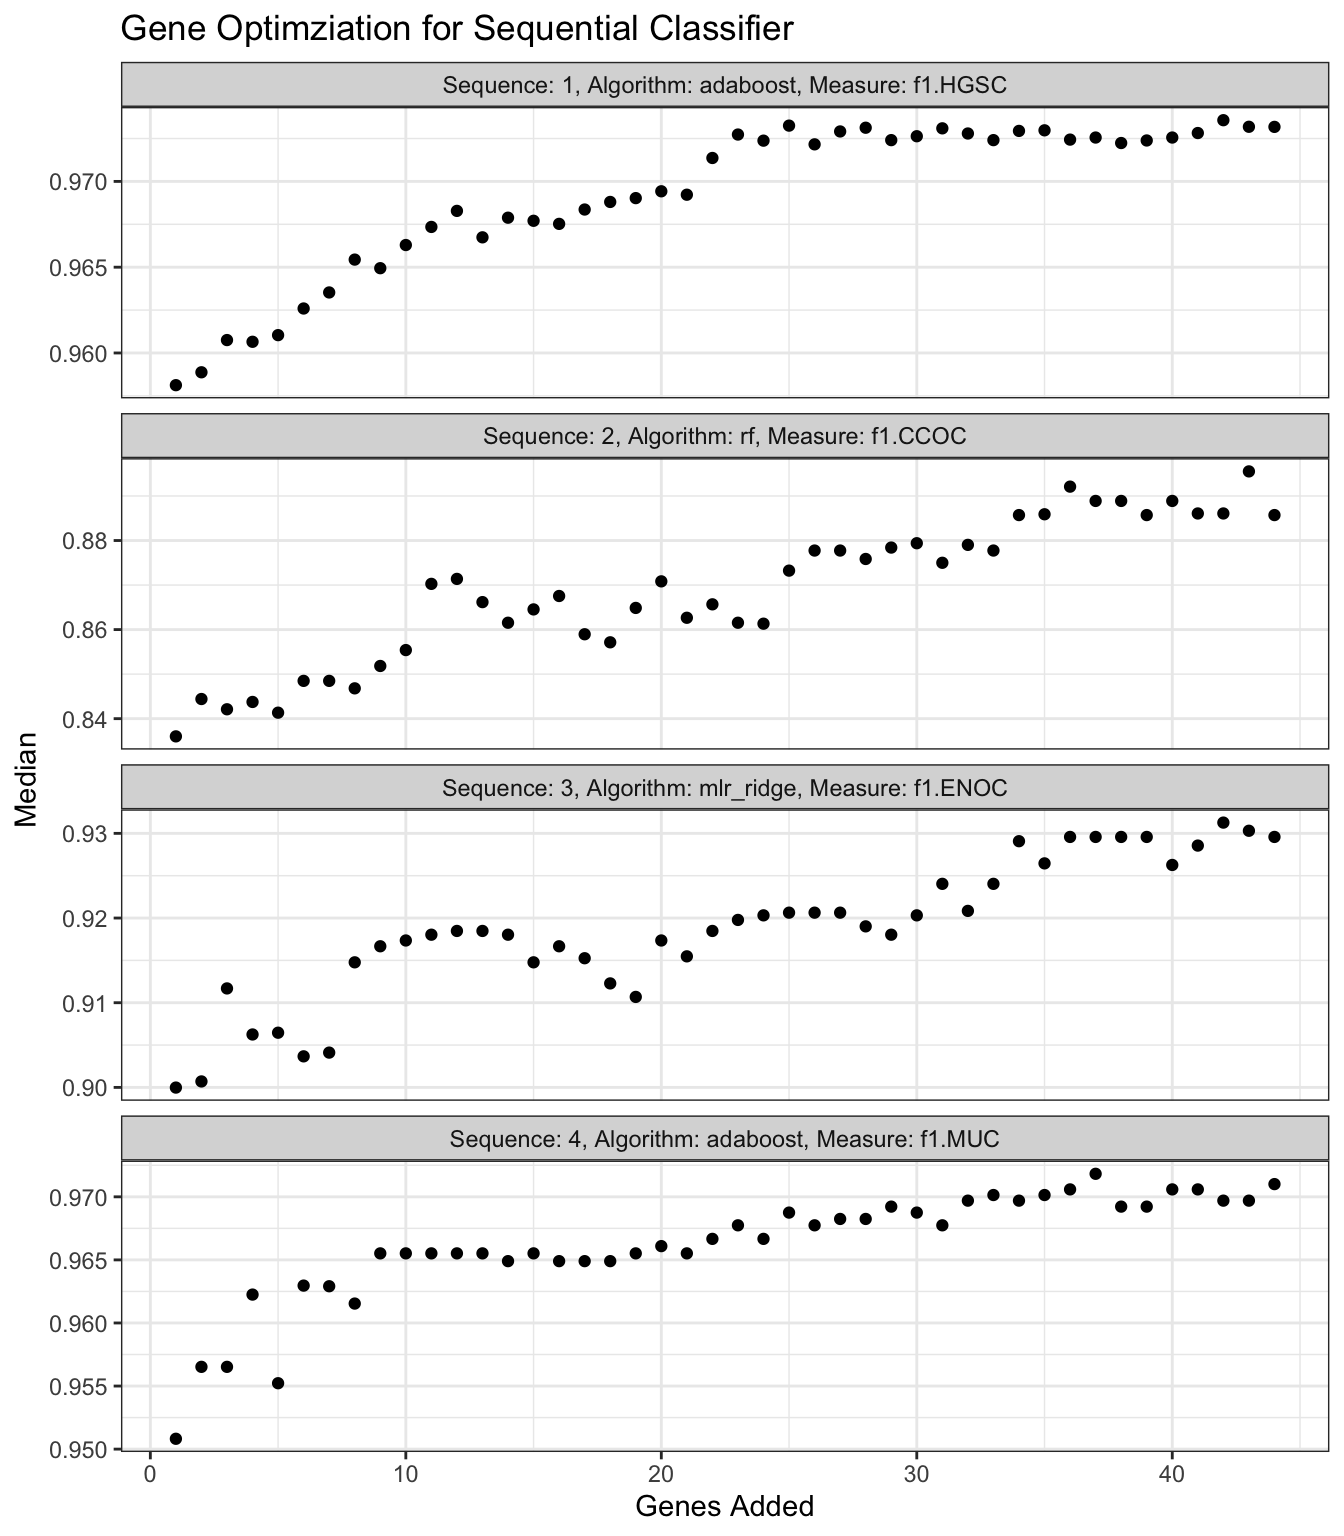
\includegraphics{OV_Histotypes_RSF_files/figure-latex/gene-seq-1} 

}

\caption{Gene Optimization for Sequential Classifier}\label{fig:gene-seq}
\end{figure}

In the sequential algorithm, sequences 1, 2, and 4 have relatively flat average F1-scores across the number of genes added. However, we can observe in sequence 3, the F1-score stabilizes at around 0.9 when we reach 13 genes added, hence the optimal number of genes used will be n=28+13=41 The added genes are: CYP2C18, TFF3, KLK7, HNF1B, IL6, IGFBP1, SLC3A1, SERPINA5, WT1, CPNE8, EGFL6, GPR64 and MUC5B.

\subsection{Two-Step Algorithm}\label{two-step-algorithm-1}

\begin{figure}[H]

{\centering 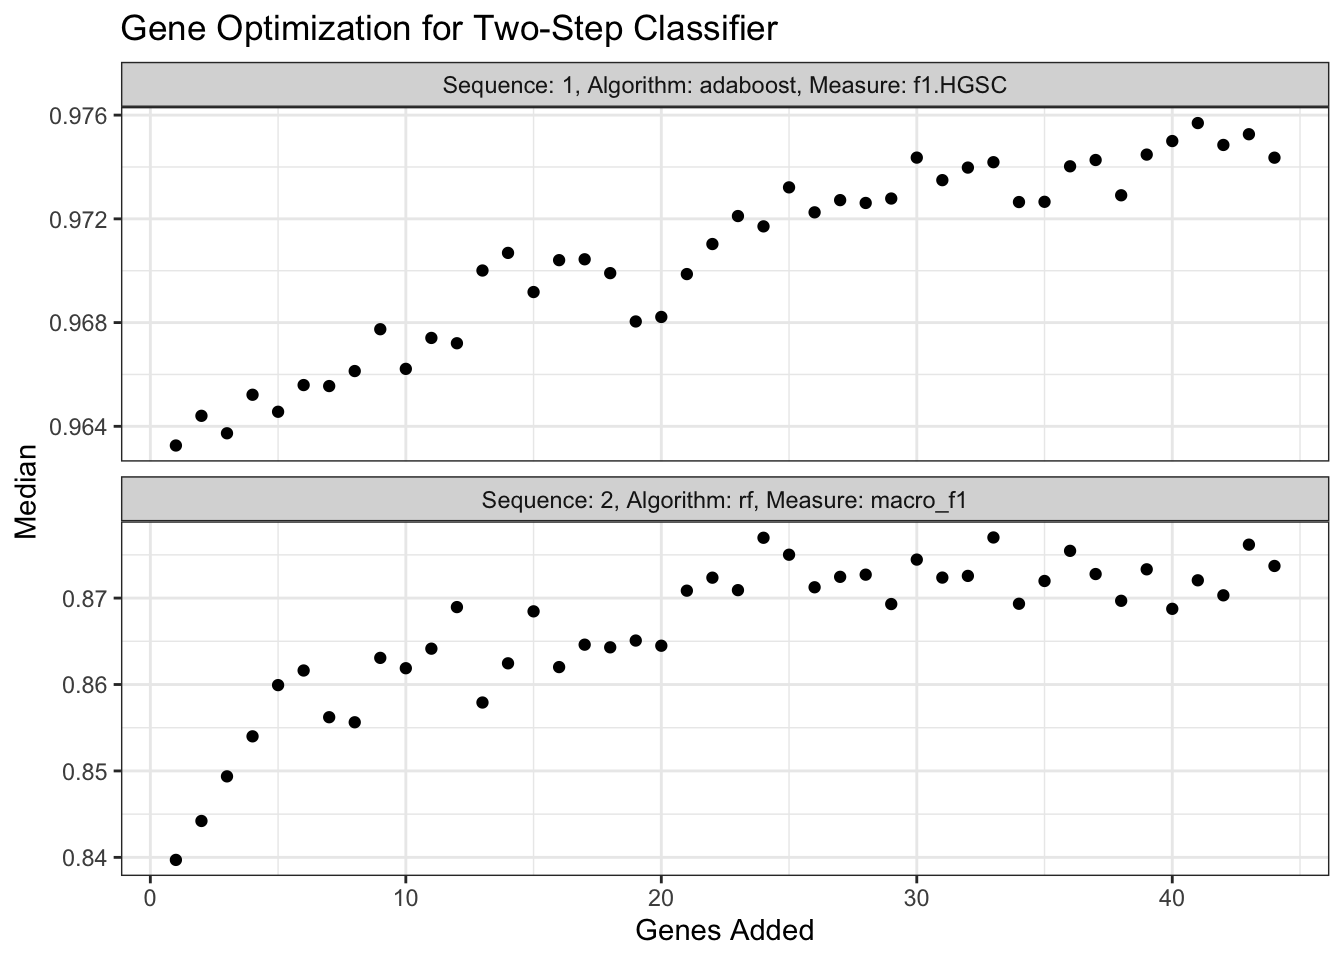
\includegraphics{OV_Histotypes_RSF_files/figure-latex/gene-2s-1} 

}

\caption{Gene Optimization for Two-Step Classifier}\label{fig:gene-2s}
\end{figure}

Since the second step of the classifier fits a multinomial model, we use the macro F1-score as the measure to analyze gene entry. In the two-step classifier, we see that in Step 2, the F1-score stabilizes at around 0.85 when we reach 12 added. The optimal number of genes used will be n=28+12=40. The added genes are: CYP2C18, MUC5B, HNF1B, SLC3A1, IGFBP1, WT1, EGFL6, TFF3, MET, KLK7, CPNE8 and STC1.

\section{Test Set Performance}\label{test-set-performance}

Now we'd like to see how our best methods perform in the confirmation and validation sets. The class-specific F1-scores will be used.

The top 2 methods are:

\begin{itemize}
\tightlist
\item
  \textbf{sequential}: sequential algorithm with hybrid subsampling at every step. The sequence of algorithms used are:

  \begin{itemize}
  \tightlist
  \item
    HGSC vs.~non-HGSC using random forest
  \item
    CCOC vs.~non-CCOC using XGBoost
  \item
    ENOC vs.~non-ENOC using support vector machine
  \item
    LGSC vs.~MUC using support vector machine
  \end{itemize}
\item
  \textbf{two\_step}: two-step algorithm with hybrid subsampling at both steps. The sequence of algorithms used are:

  \begin{itemize}
  \tightlist
  \item
    HGSC vs.~non-HGSC using random forest
  \item
    CCOC vs.~ENOC vs.~MUC vs.~LGSC support vector machine
  \end{itemize}
\end{itemize}

We can test 2 additional methods by using either the full set of genes or the optimal set of genes for both of these methods.

\subsection{Confirmation Set}\label{confirmation-set}

\begin{table}

\caption{\label{tab:conf-eval-overall}Overall Evaluation Metrics on Confirmation Set Models}
\centering
\begin{tabular}[t]{l|r|r|r|r|r|r|r}
\hline
Method & accuracy & sensitivity & specificity & f1 & bal\_accuracy & kappa & gmean\\
\hline
sequential\_full & 0.837 & 0.667 & 0.932 & 0.670 & 0.799 & 0.676 & 0.619\\
\hline
sequential\_optimal & 0.826 & 0.641 & 0.927 & 0.658 & 0.784 & 0.652 & 0.595\\
\hline
two\_step\_full & 0.837 & 0.680 & 0.932 & 0.686 & 0.806 & 0.676 & 0.645\\
\hline
two\_step\_optimal & 0.823 & 0.658 & 0.928 & 0.659 & 0.793 & 0.648 & 0.621\\
\hline
\end{tabular}
\end{table}

\begin{figure}[H]

{\centering 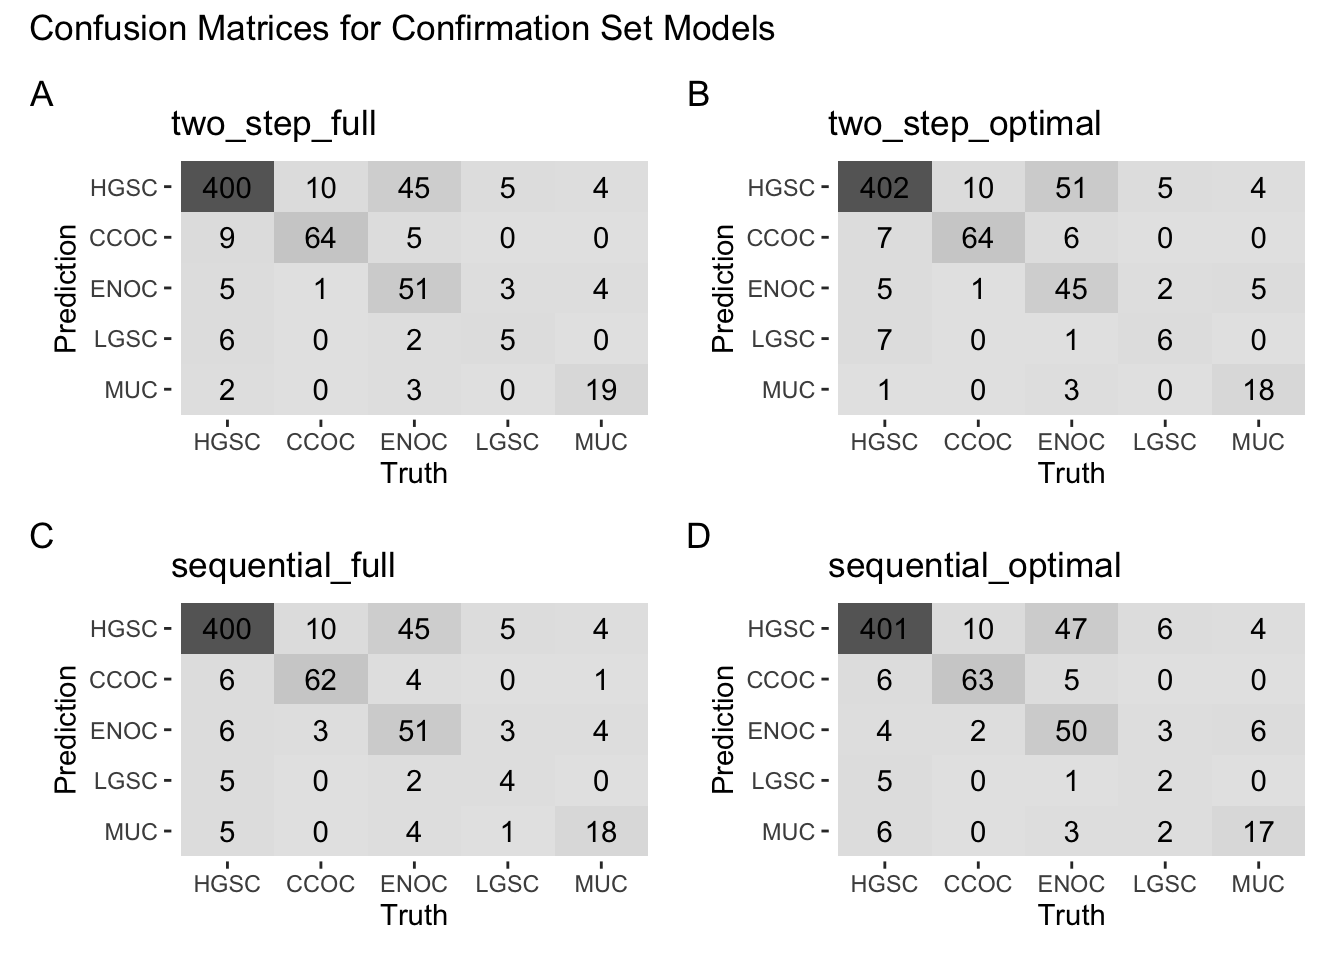
\includegraphics{OV_Histotypes_RSF_files/figure-latex/conf-conf-mat-1} 

}

\caption{Confusion Matrices for Confirmation Set Models}\label{fig:conf-conf-mat}
\end{figure}

\begin{table}

\caption{\label{tab:conf-eval-per-class}Per-Class Evaluation Metrics on Confirmation Set Model}
\centering
\begin{tabular}[t]{l|l|r|r|r|r|r}
\hline
\multicolumn{2}{c|}{ } & \multicolumn{5}{c}{Histotypes} \\
\cline{3-7}
Method & Metric & HGSC & CCOC & ENOC & LGSC & MUC\\
\hline
 & accuracy & 0.869 & 0.958 & 0.897 & 0.970 & 0.978\\
\cline{2-7}
 & sensitivity & 0.936 & 0.867 & 0.509 & 0.385 & 0.704\\
\cline{2-7}
 & specificity & 0.742 & 0.970 & 0.974 & 0.983 & 0.990\\
\cline{2-7}
 & f1 & 0.904 & 0.828 & 0.621 & 0.345 & 0.731\\
\cline{2-7}
 & bal\_accuracy & 0.839 & 0.918 & 0.742 & 0.684 & 0.847\\
\cline{2-7}
 & kappa & 0.701 & 0.804 & 0.565 & 0.330 & 0.719\\
\cline{2-7}
\multirow{-7}{*}{\raggedright\arraybackslash two\_step\_full} & gmean & 0.833 & 0.917 & 0.704 & 0.615 & 0.835\\
\cline{1-7}
 & accuracy & 0.865 & 0.946 & 0.891 & 0.966 & 0.978\\
\cline{2-7}
 & sensitivity & 0.934 & 0.853 & 0.453 & 0.385 & 0.667\\
\cline{2-7}
 & specificity & 0.733 & 0.958 & 0.978 & 0.978 & 0.992\\
\cline{2-7}
 & f1 & 0.901 & 0.785 & 0.578 & 0.312 & 0.720\\
\cline{2-7}
 & bal\_accuracy & 0.833 & 0.906 & 0.715 & 0.681 & 0.829\\
\cline{2-7}
 & kappa & 0.690 & 0.754 & 0.521 & 0.296 & 0.709\\
\cline{2-7}
\multirow{-7}{*}{\raggedright\arraybackslash two\_step\_optimal} & gmean & 0.827 & 0.904 & 0.665 & 0.613 & 0.813\\
\cline{1-7}
 & accuracy & 0.869 & 0.964 & 0.899 & 0.975 & 0.966\\
\cline{2-7}
 & sensitivity & 0.936 & 0.867 & 0.519 & 0.308 & 0.704\\
\cline{2-7}
 & specificity & 0.742 & 0.977 & 0.974 & 0.989 & 0.977\\
\cline{2-7}
 & f1 & 0.904 & 0.850 & 0.629 & 0.333 & 0.633\\
\cline{2-7}
 & bal\_accuracy & 0.839 & 0.922 & 0.746 & 0.648 & 0.840\\
\cline{2-7}
 & kappa & 0.701 & 0.829 & 0.573 & 0.321 & 0.616\\
\cline{2-7}
\multirow{-7}{*}{\raggedright\arraybackslash sequential\_full} & gmean & 0.833 & 0.920 & 0.711 & 0.552 & 0.829\\
\cline{1-7}
 & accuracy & 0.865 & 0.960 & 0.882 & 0.978 & 0.967\\
\cline{2-7}
 & sensitivity & 0.936 & 0.840 & 0.491 & 0.308 & 0.630\\
\cline{2-7}
 & specificity & 0.729 & 0.975 & 0.959 & 0.992 & 0.982\\
\cline{2-7}
 & f1 & 0.901 & 0.829 & 0.578 & 0.364 & 0.618\\
\cline{2-7}
 & bal\_accuracy & 0.832 & 0.908 & 0.725 & 0.650 & 0.806\\
\cline{2-7}
 & kappa & 0.689 & 0.806 & 0.512 & 0.353 & 0.601\\
\cline{2-7}
\multirow{-7}{*}{\raggedright\arraybackslash sequential\_optimal} & gmean & 0.826 & 0.905 & 0.686 & 0.552 & 0.786\\
\hline
\end{tabular}
\end{table}

\begin{figure}[H]

{\centering 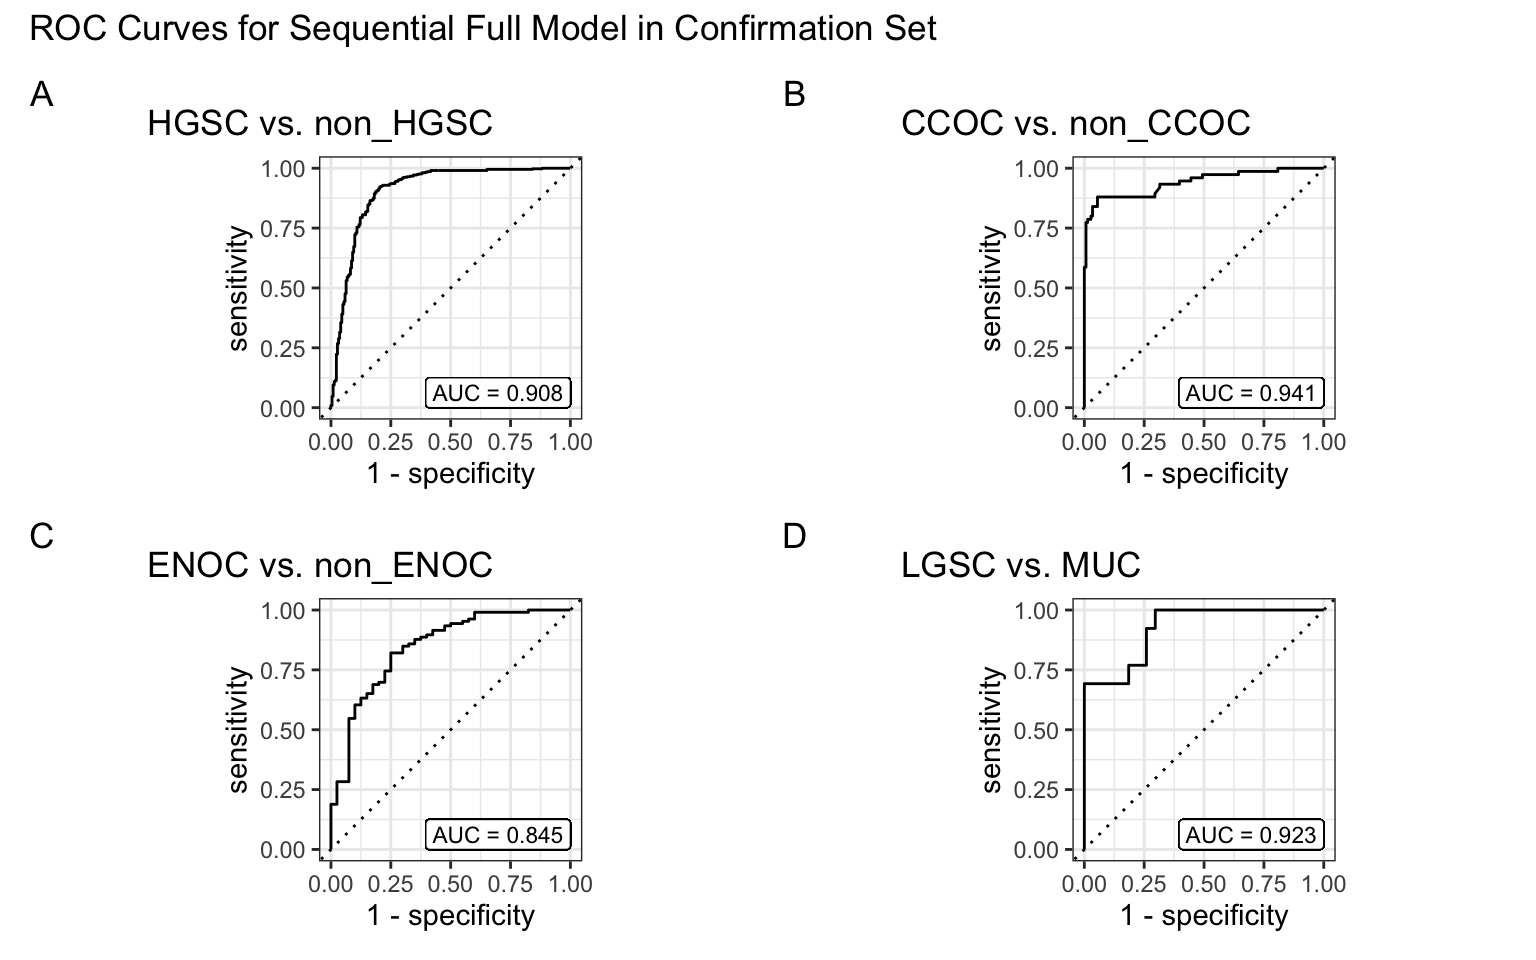
\includegraphics[width=1\linewidth]{OV_Histotypes_RSF_files/figure-latex/roc-curve-seq-full-1} 

}

\caption{ROC Curves for Sequential Full Model in Confirmation Set}\label{fig:roc-curve-seq-full}
\end{figure}

\begin{figure}[H]

{\centering 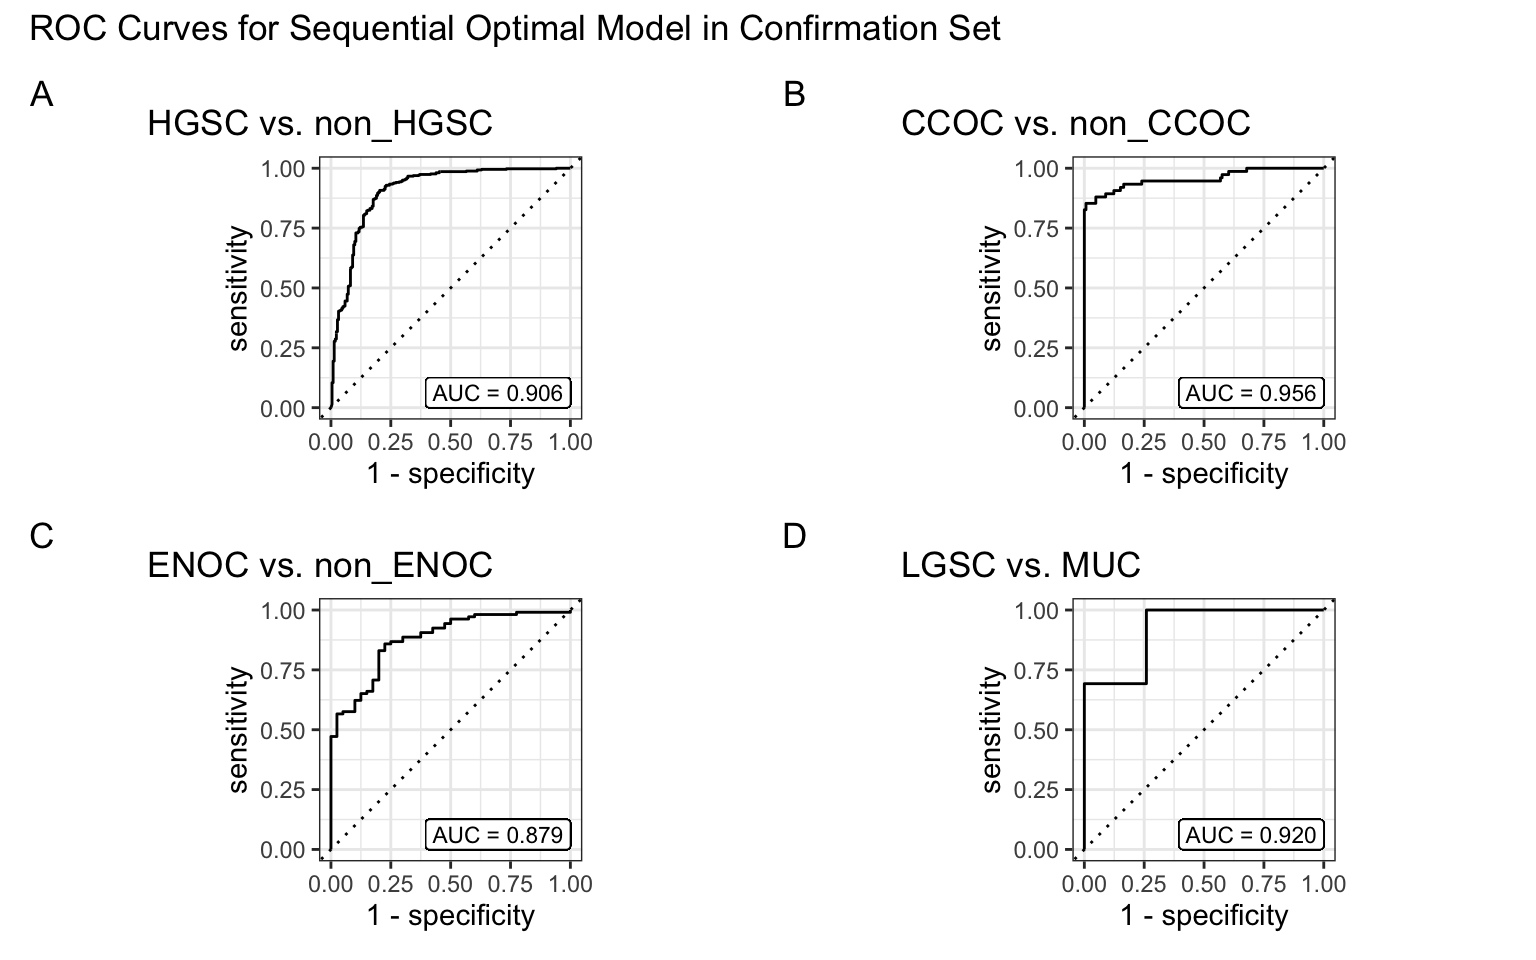
\includegraphics[width=1\linewidth]{OV_Histotypes_RSF_files/figure-latex/roc-curve-seq-opt-1} 

}

\caption{ROC Curves for Sequential Optimal Model in Confirmation Set}\label{fig:roc-curve-seq-opt}
\end{figure}

\begin{figure}[H]

{\centering 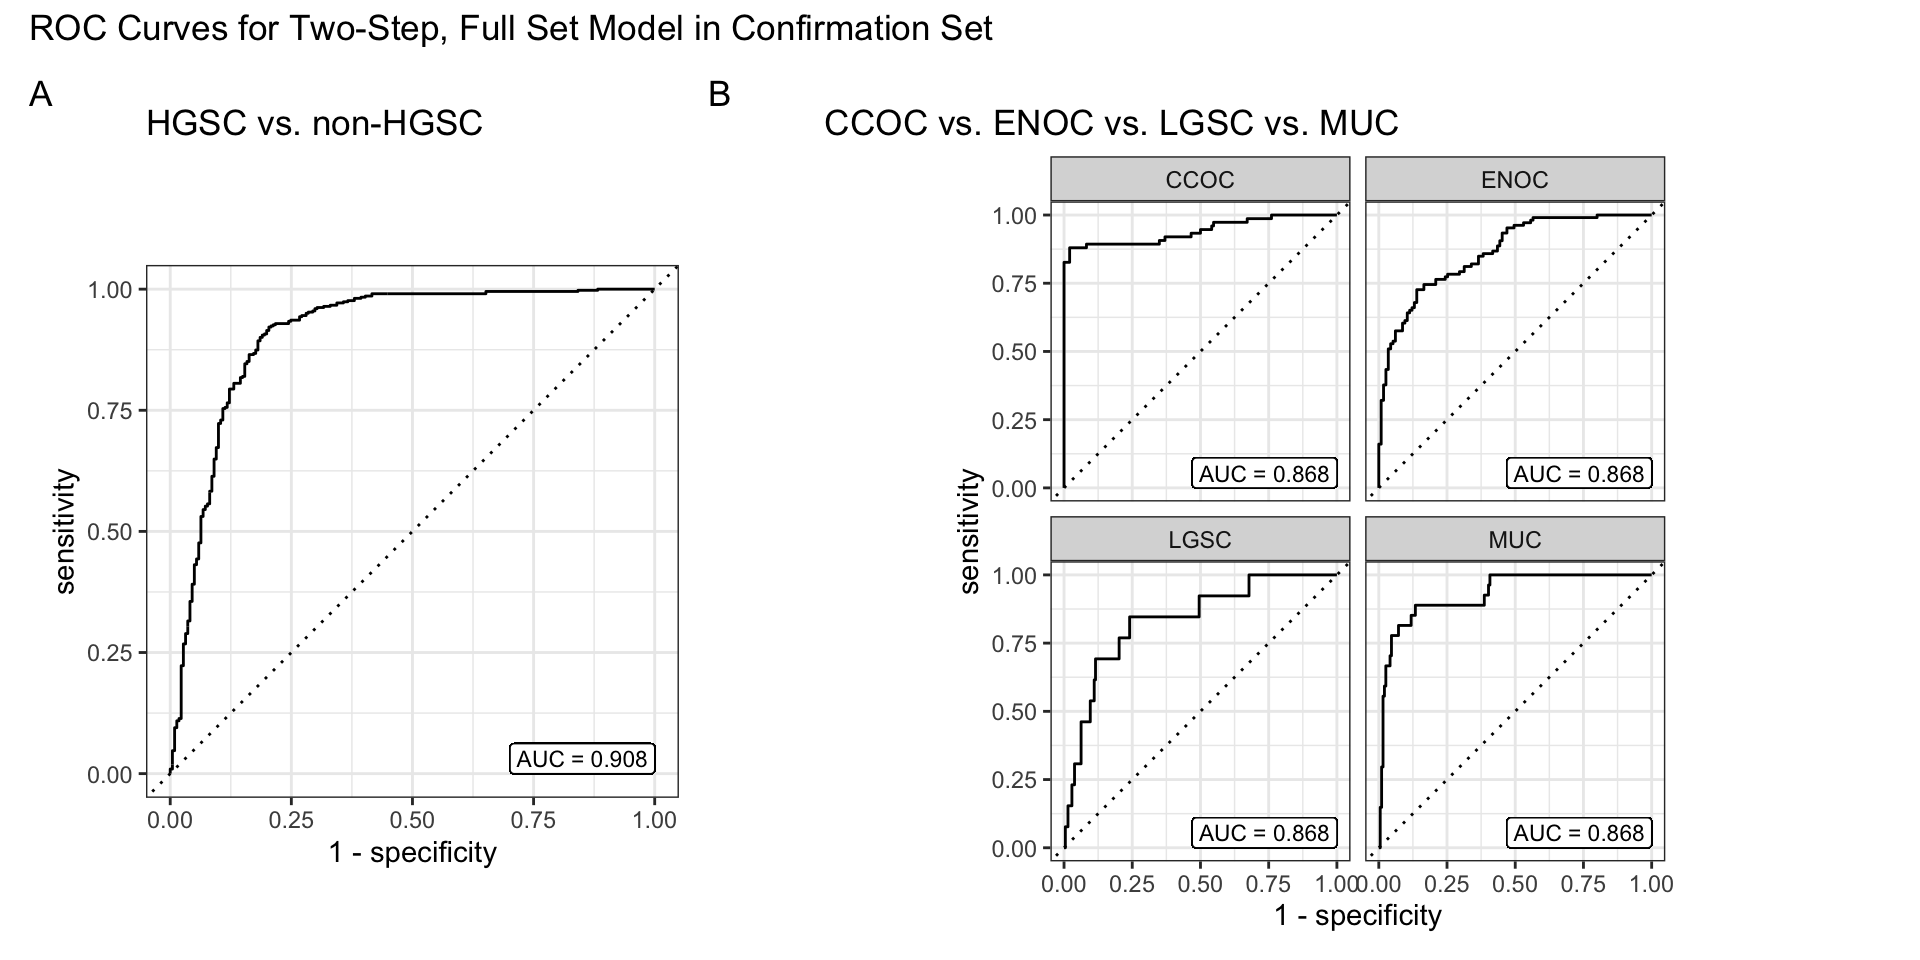
\includegraphics[width=1\linewidth]{OV_Histotypes_RSF_files/figure-latex/roc-curve-two-step-full-1} 

}

\caption{ROC Curves for Two-Step Full Model in Confirmation Set}\label{fig:roc-curve-two-step-full}
\end{figure}

\begin{figure}[H]

{\centering 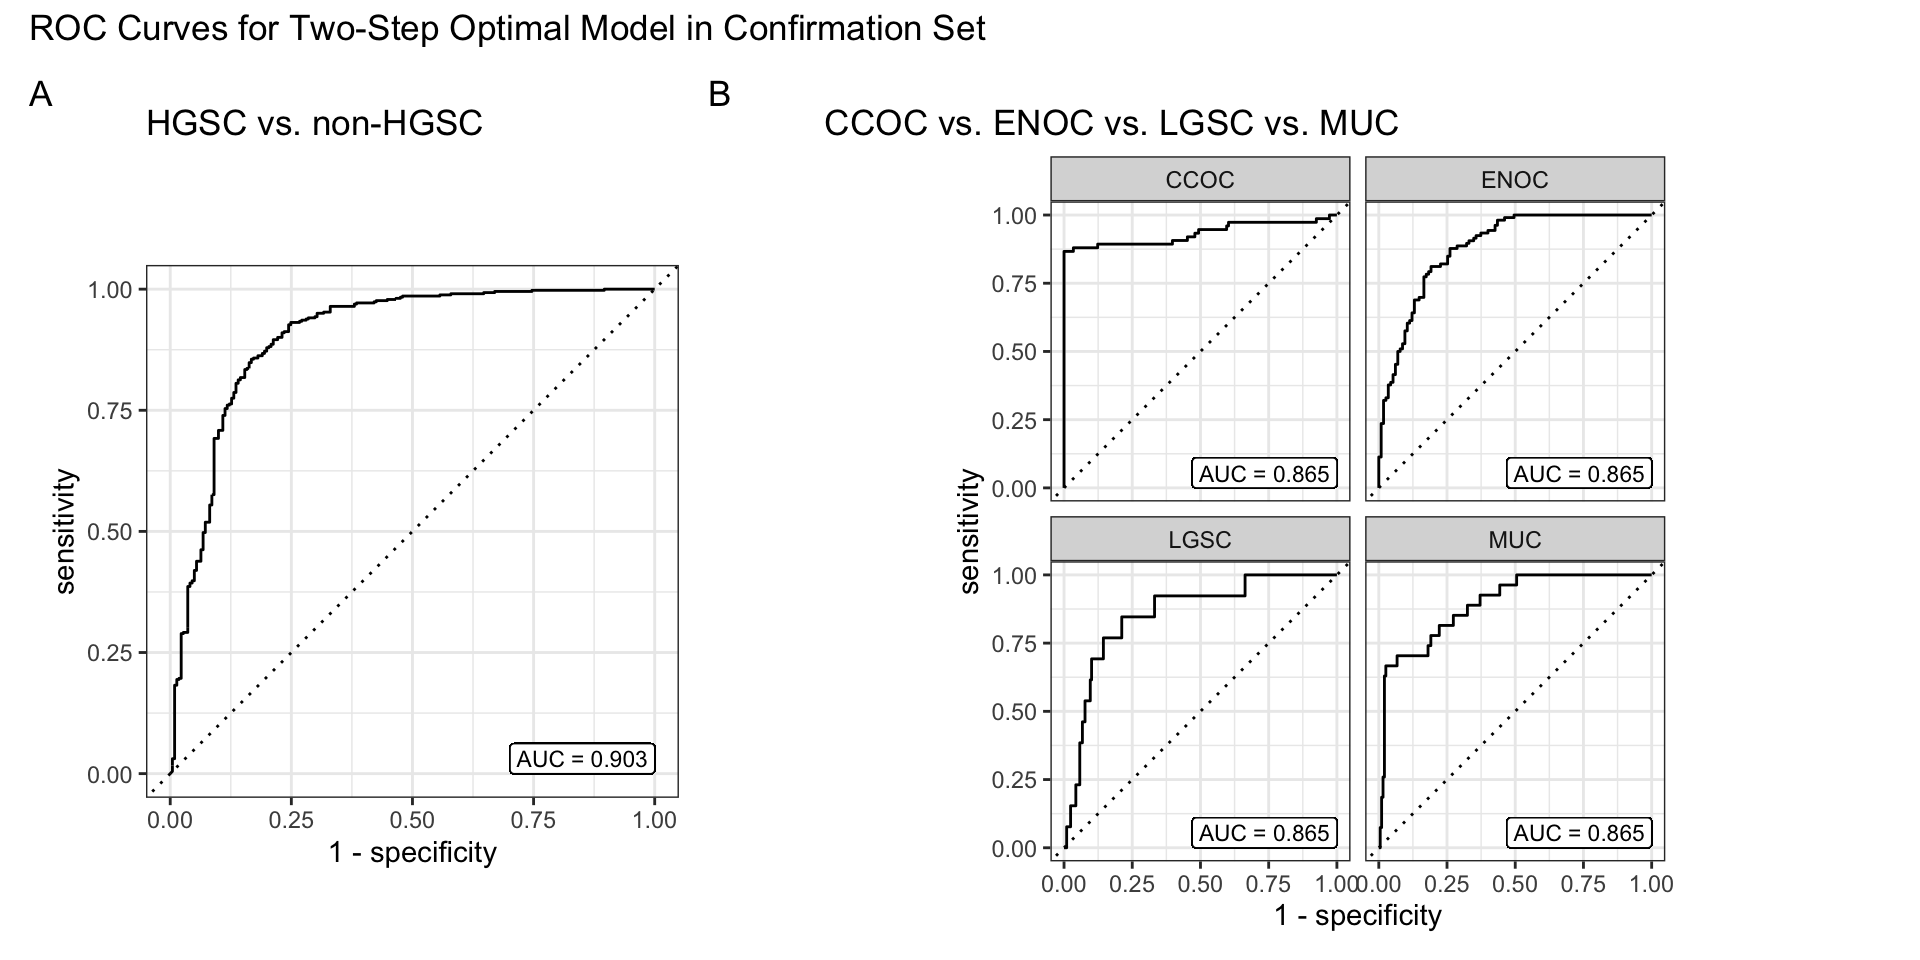
\includegraphics[width=1\linewidth]{OV_Histotypes_RSF_files/figure-latex/roc-curve-two-step-opt-1} 

}

\caption{ROC Curves for Two-Step Optimal Model in Confirmation Set}\label{fig:roc-curve-two-step-opt}
\end{figure}

\subsection{Validation Set}\label{validation-set}

\begin{table}

\caption{\label{tab:val-eval-overall}Overall Evaluation Metrics on Validation Set Model}
\centering
\begin{tabular}[t]{l|r|r|r|r|r|r|r}
\hline
Method & accuracy & sensitivity & specificity & f1 & bal\_accuracy & kappa & gmean\\
\hline
two\_step\_optimal & 0.851 & 0.729 & 0.939 & 0.663 & 0.834 & 0.663 & 0.7\\
\hline
\end{tabular}
\end{table}

\begin{figure}[H]

{\centering 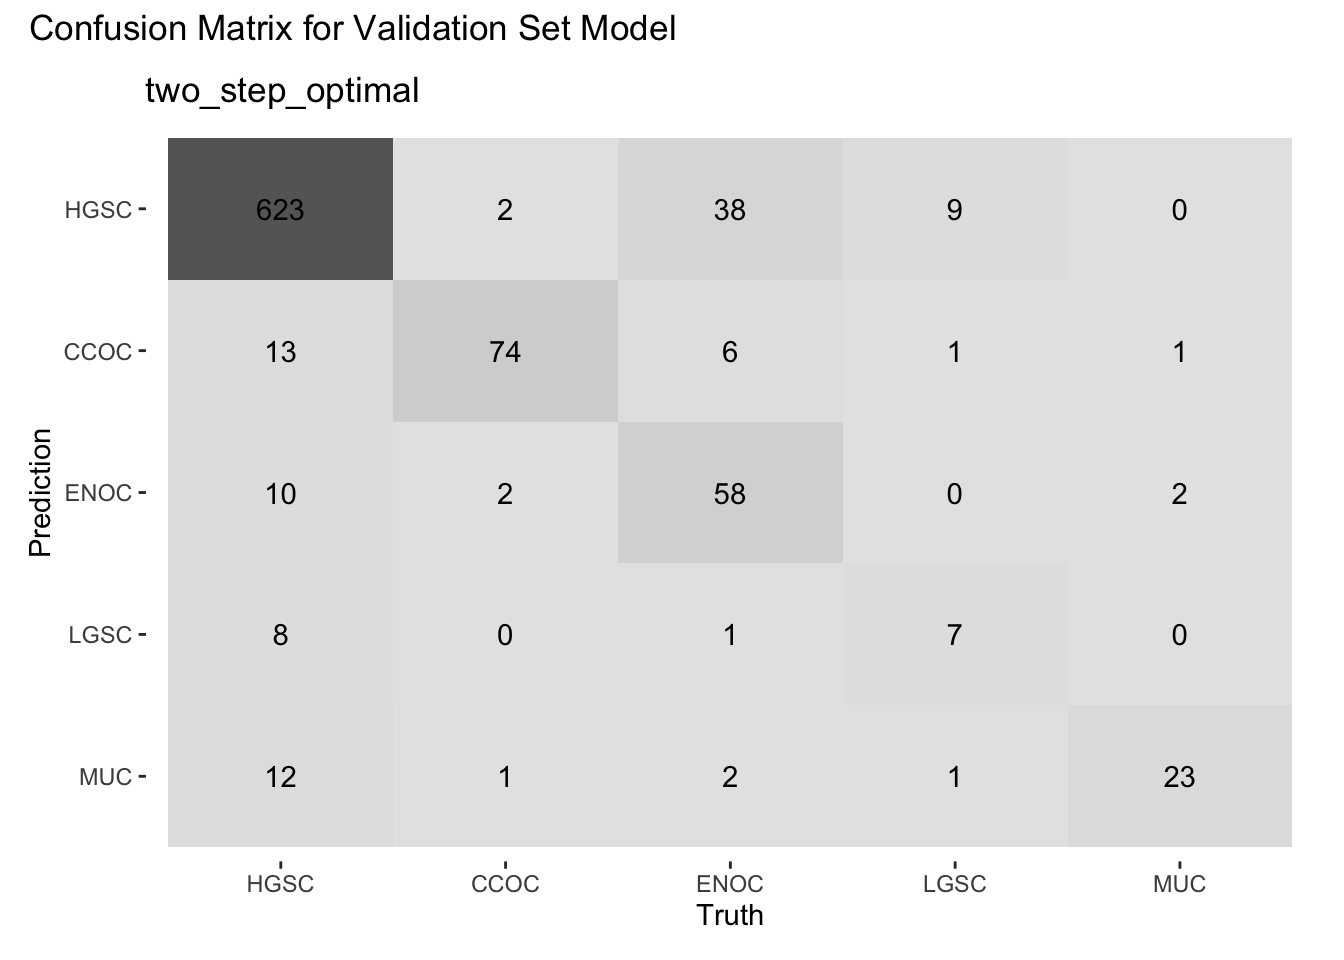
\includegraphics{OV_Histotypes_RSF_files/figure-latex/val-conf-mat-1} 

}

\caption{Confusion Matrix for Validation Set Model}\label{fig:val-conf-mat}
\end{figure}

\begin{table}

\caption{\label{tab:val-eval-per-class}Per-Class Eevaluation Metrics on Validation Set Model}
\centering
\begin{tabular}[t]{l|l|r|r|r|r|r}
\hline
\multicolumn{2}{c|}{ } & \multicolumn{5}{c}{Histotypes} \\
\cline{3-7}
Method & Metric & HGSC & CCOC & ENOC & LGSC & MUC\\
\hline
 & accuracy & 0.875 & 0.967 & 0.928 & 0.971 & 0.960\\
\cline{2-7}
 & sensitivity & 0.901 & 0.938 & 0.556 & 0.444 & 0.808\\
\cline{2-7}
 & specificity & 0.802 & 0.970 & 0.979 & 0.982 & 0.965\\
\cline{2-7}
 & f1 & 0.915 & 0.833 & 0.649 & 0.381 & 0.538\\
\cline{2-7}
 & bal\_accuracy & 0.851 & 0.954 & 0.767 & 0.713 & 0.886\\
\cline{2-7}
 & kappa & 0.682 & 0.815 & 0.610 & 0.367 & 0.520\\
\cline{2-7}
\multirow{-7}{*}{\raggedright\arraybackslash two\_step\_optimal} & gmean & 0.850 & 0.953 & 0.737 & 0.661 & 0.883\\
\hline
\end{tabular}
\end{table}

  \bibliography{book.bib,packages.bib}
\addcontentsline{toc}{chapter}{\bibname}

\end{document}
